%%% LaTeX-Vorlage Version 2.1 %%%

% TODO: individuelle Einstellungen (Name, Titel etc.)
% -> bitte in Konfigurationsdatei anpassen
%%%%
%
% Zentrale Konfigurationsdatei
%
% In dieser Datei sind eine Reihe verpflichtender Einstellungen 
% (Nr. 1 bis 6) vorzunehmen.
%
% Die Einstellungen unter Nr. 7 bis 11 können im Regelfall unverändert
% belassen werden. Ausnahmen sind:
%  - Ihre Arbeit ist in englischer Sprache verfasst (Nr. 7)
%  - der Titel Ihrer Arbeit ist sehr lang, so dass er nicht auf das
%    Deckblatt passt oder anders umgebrochen werden soll (Nr. 8 und 9)
%  - es soll ein besonderes Abgabedatum angegeben werden (Nr. 10)
%  - Sie benötigen einen Vertraulichkeitsvermerk (Nr. 11)
%
%%%%


% TODO 1. Typ der Arbeit (für Titelseite und Metadaten)
% Zutreffendes auswählen:

%\newcommand{\typMeinerArbeit}{PA1} 
%\newcommand{\typMeinerArbeit}{PA2} 
%\newcommand{\typMeinerArbeit}{Seminararbeit} 
\newcommand{\typMeinerArbeit}{PA1} 

% TODO 2. Vorname, Name der Autorin/des Autors (für Deckblatt und Metadaten)
\newcommand{\meinName}{Felix Wolfram}

% TODO 3. Kurs eintragen
\newcommand{\meinKurs}{WWI2024F}

% TODO 4. Titel der Arbeit (für Deckblatt, ehrenwörtliche Erklärung und Metadaten, ohne Umbrüche angeben)
\newcommand{\themaMeinerArbeit}{Entwicklung und Evaluation von KI-Modellen auf Basis synthetischer Daten aus digitalen Modellen zur Fehlererkennung bei Werkzeugmaschinen}

% TODO 5. Angaben zum Unternehmen (wird bei Seminararbeiten nicht angezeigt)
\newcommand{\UNName}{TRUMPF SE + Co. KG}
\newcommand{\UNBetreuer}{Tom Körner}
\newcommand{\UNBetreuerFunktion}{}

% TODO 6. Angaben zur wissenschaftlichen Betreuung 
\newcommand{\DHBWBetreuer}{Prof. Dr. Kai Holzweißig}


% OPTIONALE Einstellungen

% 7. Arbeit in Englisch
% (nur ändern, falls Ihre Arbeit in englischer Sprache geschrieben ist)
\newcommand{\meineSprache}{DE}	% Standard-Einstellung
%\newcommand{\meineSprache}{EN}	% für Arbeiten in englischer Sprache

% 8. Schriftgröße des Titels auf Deckblatt
% (nur ändern, falls Sie einen sehr langen Titel haben)
% Zutreffendes auswählen:
\newcommand{\schriftgroesseTitel}{\LARGE}   % Standard-Einstellung
%\newcommand{\schriftgroesseTitel}{\Large}  % bei sehr langen Titeln

% 9. Titel mit Umbrüchen für Deckblatt
% (nur ändern, falls Sie den Zeilenumbruch selbst beeinflussen möchten)
\newcommand{\titelAufDeckblatt}{\themaMeinerArbeit}		% Standard-Einstellung
%\newcommand{\titelAufDeckblatt}{Herausforderungen der Digitalisierung im globalen Wettbewerb von Industrieunternehmen \\ -- eine vergleichende Untersuchung unter Berücksichtigung aktueller und weniger aktueller Forschungsmethoden \\ am Beispiel der Firma Melanie Müller und Söhne AG} % explizite Angabe

% 10. Abgabedatum anpassen
% Zutreffendes auswählen:
\newcommand{\abgabeDatum}{\today}  		% Standard-Einstellung
%\newcommand{\abgabeDatum}{TT.MM.JJJJ}  % falls nicht aktuelles Datum

% 11. Vertraulichkeitsvermerk
% (nur ändern, falls Ihre Arbeit einen Vertraulichkeitsvermerk tragen soll)
\newcommand{\hatVermerk}{nein}  	% Standard-Einstellung
% \newcommand{\hatVermerk}{ja}  	% falls Vertraulichkeitsvermerk


% Grundlegende Dokumenteneigenschaften gemäß DHBW-Vorgaben
\documentclass[a4paper,fontsize=11pt,oneside,parskip=half,headings=normal,listof=nochaptergap]{scrreprt} 
% \usepackage{showframe} % nur für Kontrolle der Ränder 

%%% Präambel einbinden (mit Festlegungen gemäß DHBW-Vorgaben) %%%
%%% Präambel %%%
% hier sollten keine Änderungen erforderlich sein
%
\usepackage{ifthen}           % für Umschaltung DE/EN
\newcommand{\DEoEN}[2]{\ifthenelse{\equal{\meineSprache}{DE}}{#1}{#2}}

\usepackage{tabularx}   % flexible Tabellenbreiten
\usepackage{array}      % p-Spalten & \arraybackslash
\usepackage{enumitem}   % Listen-Feintuning
\usepackage{tikz}       % Checkboxen zeichnen

\usepackage{subcaption}

% kleine Hilfen
\newcolumntype{Y}{>{\raggedright\arraybackslash}X}
\renewcommand{\arraystretch}{1.25}

% Checkbox-Symbol (klein, passt in Text)
\newcommand{\checkedbox}{%
  \tikz[scale=0.9,baseline=-0.6ex] \draw (0,0) rectangle (0.22,0.22)
    (0.03,0.12) -- (0.09,0.04) -- (0.19,0.20);%
}

\usepackage[utf8]{inputenc}   % Zeichencodierung UTF-8 für Eingabe-Dateien
\usepackage[T1]{fontenc}      % Darstellung von Umlauten im PDF

\usepackage{listings}         % für Einbindung von Code-Listings
\lstset{numbers=left,numberstyle=\tiny,numbersep=5pt,texcl=true}
\lstset{literate=             % erlaubt Sonderzeichen in Code-Listings 
{Ö}{{\"O}}1
{Ä}{{\"A}}1
{Ü}{{\"U}}1
{ß}{{\ss}}2
{ü}{{\"u}}1
{ä}{{\"a}}1
{ö}{{\"o}}1
{€}{{\euro}}1
}

\usepackage[
  inner=35mm,outer=15mm,top=25mm,
  bottom=20mm,foot=12mm,includefoot
]{geometry}                 % Einstellungen für Ränder

\DEoEN{
  \usepackage[ngerman]{babel} % Spracheinstellungen Deutsch
  \usepackage[babel,german=quotes]{csquotes} % deutsche Anf.zeichen
}{
 \usepackage[english]{babel} % Spracheinstellungen Englisch
 \usepackage[babel,english=british]{csquotes} % englische Anf.zeichen
}

\usepackage{enumerate}      % anpassbare Nummerier./Aufz.
\usepackage{graphicx}       % Einbinden von Grafiken
\usepackage[onehalfspacing]{setspace} % anderthalbzeilig

\usepackage{blindtext}      % Textgenerierung für Testzwecke
\usepackage{color}          % Verwendung von Farbe 

\usepackage[                % Biblatex
  backend=biber,
  bibstyle=_dhbw_authoryear,maxbibnames=99,
  citestyle=authoryear, dashed=false,    
  uniquename=true, useprefix=true,
  bibencoding=utf8]{biblatex}
%kein Punkt am Ende bei \footcite
%http://www.golatex.de/footcite-ohne-punkt-am-schluss-t4865.html
\renewcommand{\bibfootnotewrapper}[1]{\bibsentence#1}

% Bibliographie: Vornamen ausgeschrieben
\DeclareNameAlias{author}{family-given}
\DeclareNameAlias{editor}{family-given}

%Reihenfolge der Autorennamen
%   
% http://golatex.de/viewtopic,p,80448.html#80448
% Argumente: siehe http://texwelt.de/blog/modifizieren-eines-biblatex-stils/
\DeclareNameFormat{sortname}{% Bibliographie
  \ifnum\value{uniquename}=0 % Normalfall
    \ifuseprefix%
      {%
         \usebibmacro{name:family-given}
           {\namepartfamily}
           {\namepartgiveni}
           {\namepartprefix}
           {\namepartsuffixi}%
       }
      {%
         \usebibmacro{name:family-given}
           {\namepartfamily}
           {\namepartgiveni}
           {\namepartprefixi}
           {\namepartsuffixi}%
       }%
  \fi
  \ifnum\value{uniquename}=1% falls nicht eindeutig, abgek. Vorname 
      {%
         \usebibmacro{name:family-given}
           {\namepartfamily}
           {\namepartgiveni}
           {\namepartprefix}
           {\namepartsuffix}%
       }%
  \fi
  \ifnum\value{uniquename}=2% falls nicht eindeutig, ganzer Vorname 
      {%
         \usebibmacro{name:family-given}
           {\namepartfamily}
           {\namepartgiven}
           {\namepartprefix}
           {\namepartsuffix}%
       }%
  \fi   
  \usebibmacro{name:andothers}}

\DeclareNameFormat{labelname}{% für Zitate
  \ifnum\value{uniquename}=0 % Normalfall
    \ifuseprefix%
      {%
         \usebibmacro{name:family-given}
           {\namepartfamily}
           {\empty}
           {\namepartprefix}
           {\namepartsuffixi}%
       }
      {%
         \usebibmacro{name:family-given}
           {\namepartfamily}
           {\empty}
           {\namepartprefixi}
           {\namepartsuffixi}%
       }%
  \fi
  \ifnum\value{uniquename}=1% falls nicht eindeutig, abgek. Vorname 
      {%
         \usebibmacro{name:family-given}
           {\namepartfamily}
           {\namepartgiveni}
           {\namepartprefix}
           {\namepartsuffix}%
       }%
  \fi
  \ifnum\value{uniquename}=2% falls nicht eindeutig, ganzer Vorname 
      {%
         \usebibmacro{name:family-given}
           {\namepartfamily}
           {\namepartgiven}
           {\namepartprefix}
           {\namepartsuffix}%
       }%
  \fi   
  \usebibmacro{name:andothers}}
      
  
\DeclareFieldFormat{extrayear}{% = the 'a' in 'Jones 1995a'
  \iffieldnums{labelyear}
    {\mknumalph{#1}}
    {\mknumalph{#1}}}        

% Namen getrennt durch Komma (Zitate)
\DeclareDelimFormat*[footcite,cite,textcite,parencite]{multinamedelim}{\addcomma\space}
% bzw. Semikolon (Literaturverzeichnis)
\DeclareDelimFormat[bib,biblist]{multinamedelim}{\addsemicolon\space}
% keine besondere Behandlung beim letzten Autor
\DeclareDelimAlias{finalnamedelim}{multinamedelim}
%\DeclareDelimAlias{multilistdelim}{multinamedelim}

\renewcommand{\nameyeardelim}{~}

% Literaturverzeichnis: Doppelpunkt zwischen Name (Jahr): Rest 
% http://de.comp.text.tex.narkive.com/Tn1HUIXB/biblatex-authoryear-und-doppelpunkt
\renewcommand{\labelnamepunct}{\addcolon\addspace}

% damit die Darstellung für Vollzitate von Primärquellen in 
% Fußnoten später auf "nicht fett" geändert werden kann 
% (nur für Zitate von Sekundärliteratur relevant)
\newcommand{\textfett}[1]{\textbf{#1}}

% für Zitate von Sekundärliteratur:
\newcommand{\footcitePrimaerSekundaer}[4]{%
  \renewcommand{\textfett}[1]{##1}%
  \footnote{\fullcite[#2]{#1}, \DEoEN{zitiert nach}{as cited in} \cite[#4]{#3}}%  
  \renewcommand{\textfett}[1]{\textbf{##1}}%
}

% Im Literaturverzeichnis: Autor (Jahr) fett
\renewbibmacro*{author}{%
  \ifboolexpr{%
    test \ifuseauthor%
    and
    not test {\ifnameundef{author}}
  }
    {\usebibmacro{bbx:dashcheck}
       {\bibnamedash}
       {\usebibmacro{bbx:savehash}%
        \textfett{\printnames{author}}%
        \iffieldundef{authortype}
          {\setunit{\addspace}}
          {\setunit{\addcomma\space}}}%
     \iffieldundef{authortype}
       {}
       {\usebibmacro{authorstrg}%
        \setunit{\addspace}}}%
    {\global\undef\bbx@lasthash
     \usebibmacro{labeltitle}%
     \setunit*{\addspace}}%
  \textfett{\usebibmacro{date+extrayear}}}

% Sonderfall: Quelle ohne Autor, aber mit Herausgeber
% Name des Herausgebers wird fett gedruckt
\renewbibmacro*{bbx:editor}[1]{%
  \ifboolexpr{%
    test \ifuseeditor%
    and
    not test {\ifnameundef{editor}}
  }
    {\usebibmacro{bbx:dashcheck}
       {\bibnamedash}
       {\textfett{\printnames{editor}}%
        \setunit{\addcomma\space}%
        \usebibmacro{bbx:savehash}}%
     \usebibmacro{#1}%
     \clearname{editor}%
     \setunit{\addspace}}%
    {\global\undef\bbx@lasthash
     \usebibmacro{labeltitle}%
     \setunit*{\addspace}}%
  \textfett{\usebibmacro{date+extrayear}}}

\DefineBibliographyStrings{ngerman}{% Anpassungen für deutsche Sprache
	nodate = {{o.J.}},
	urlseen = {{Abruf:}},
	ibidem = {{ebenda}},
	andothers = {{et\addabbrvspace al\adddot}}
}
\DefineBibliographyStrings{english}{% Anpassungen für englische Sprache
    nodate = {{w.y.}},
    urlseen = {{retrieval:}}
}

% keine Anführungszeichen beim Titel im Literaturverzeichnis
\DeclareFieldFormat[article,book,inbook,inproceedings,manual,misc,phdthesis,thesis,online,report]{title}{#1\isdot}

\newcommand{\literaturverzeichnis}{%
% nur Literaturverzeichnis
% (als eigenes Kapitel)
\phantomsection
\addcontentsline{toc}{chapter}{\refname}
\spezialkopfzeile{\refname}
\defbibheading{lit}{\chapter*{\refname}}
\label{chapter:quellen}
\printbibliography[heading=lit,notkeyword=ausblenden]
}
 % mit DHBW-spezifischen Einstellungen

\usepackage{tocloft}        % für Verzeichnis der Anhänge

\usepackage{multirow}       % Tabellenformatierung 

\usepackage{amsmath}        % Erweiterung math. Formelsatz
\usepackage{amssymb}        % math. Symbole

\usepackage{booktabs}       % professionelle Tabellen

\usepackage[hypertexnames=false]{hyperref}       % URL-Formatierung, klickbare Verweise

\usepackage[printonlyused]{acronym}

% Anhänge
\newcounter{anhcnt}
\setcounter{anhcnt}{0}
\newlistof{anhang}{app}{}

\newcommand{\anhang}[1]{%
  \refstepcounter{anhcnt}
  \setcounter{anhteilcnt}{0}
  \section*{\appendixname\ \theanhcnt: #1}
  \addcontentsline{app}{section}{\protect\numberline{\appendixname\ \theanhcnt}#1}\par
}

\newcounter{anhteilcnt}
\setcounter{anhteilcnt}{0}

\newcommand{\anhangteil}[1]{%
	\refstepcounter{anhteilcnt}
	\subsection*{\appendixname\ \arabic{anhcnt}/\arabic{anhteilcnt}: #1}
	\addcontentsline{app}{subsection}{\protect\numberline{\appendixname\ \theanhcnt/\arabic{anhteilcnt}}#1}\par
}

\renewcommand{\theanhteilcnt}{\appendixname\ \theanhcnt/\arabic{anhteilcnt}}

% vgl. S. 4 Paket-Beschreibung tocloft 	
% Einrückungen für Anhangverzeichnis
\makeatletter
\newcommand{\abstaendeanhangverzeichnis}{
\renewcommand*{\l@section}{\@dottedtocline{1}{0em}{5.5em}}
\renewcommand*{\l@subsection}{\@dottedtocline{2}{2.3em}{6.5em}}
}
\makeatother

% Einrückungen
\makeatletter
\renewcommand*{\l@figure}{\@dottedtocline{1}{0em}{2.3em}}
\renewcommand*{\l@table}{\@dottedtocline{1}{0em}{2.3em}}
\makeatother


\usepackage{chngcntr}                % fortlaufende Zähler für Fußnoten, Abbildungen und Tabellen
\counterwithout{figure}{chapter}
\counterwithout{table}{chapter}
\counterwithout{footnote}{chapter}

\usepackage[automark]{scrlayer-scrpage} 
%% Definitionen für Kopf- und Fußzeile auf normalen Seiten
\defpagestyle{kopfzeile}
{% Kopfdefinition
  (\textwidth,0pt)    % Länge der oberen Linie,Dicke der oberen Linie       
  {} % Definition für linke Seiten im doppelseitigen Layout
  {} % Definition für rechte Seiten im doppelseitigen Layout      
  {  % Definition für Seiten im einseitigen Layout
	\makebox[0pt][l]{\rightmark}% 
	\makebox[\linewidth]{}% 
  }        
  (\textwidth, 0.4pt) % Untere Linienlänge, Untere Liniendicke
}
{% Fußdefinition
  (\textwidth,0pt)    % Obere Linienlänge, Obere Liniendicke
  {} % Definition für linke Seiten im doppelseitigen Layout
  {} % Definition für rechte Seiten im doppelseitigen Layout
  {  % Definition für Seiten im einseitigen Layout
    \makebox[\linewidth]{}%
    \makebox[0pt][r]{\pagemark}%
  }
  (\textwidth, 0pt)   % Länge der unteren Linie,Dicke der unteren Linie
}

%% Definitionen für Kopf- und Fußzeile auf ersten Seiten eines Kapitels
\defpagestyle{kapitelkopfzeile}
{% Kopfdefinition
  (\textwidth,0pt)    % Länge der oberen Linie,Dicke der oberen Linie       
  {} % Definition für linke Seiten im doppelseitigen Layout
  {} % Definition für rechte Seiten im doppelseitigen Layout      
  {}  % Definition für Seiten im einseitigen Layout
  (\textwidth, 0pt) % Untere Linienlänge, Untere Liniendicke
}
{% Fußdefinition
  (\textwidth,0pt)    % Obere Linienlänge, Obere Liniendicke
  {} % Definition für linke Seiten im doppelseitigen Layout
  {} % Definition für rechte Seiten im doppelseitigen Layout
  {  % Definition für Seiten im einseitigen Layout
    \makebox[\linewidth]{}%
    \makebox[0pt][r]{\pagemark}%
  }
  (\textwidth, 0pt)   % Länge der unteren Linie,Dicke der unteren Linie
}

%% Definitionen für Kopf- und Fußzeile im Anhang und bei Quellenverzeichnisse
\newcommand{\spezialkopfzeileBezeichnung}{}
\defpagestyle{spezialkopfzeile}
{% Kopfdefinition
  (\textwidth,0pt)    % Länge der oberen Linie,Dicke der oberen Linie       
  {} % Definition für linke Seiten im doppelseitigen Layout
  {} % Definition für rechte Seiten im doppelseitigen Layout      
  {  % Definition für Seiten im einseitigen Layout
	\makebox[0pt][l]{\spezialkopfzeileBezeichnung}% 
	\makebox[\linewidth]{}% 
  }        
  (\textwidth, 0.4pt) % Untere Linienlänge, Untere Liniendicke
}
{% Fußdefinition
  (\textwidth,0pt)    % Obere Linienlänge, Obere Liniendicke
  {} % Definition für linke Seiten im doppelseitigen Layout
  {} % Definition für rechte Seiten im doppelseitigen Layout
  {  % Definition für Seiten im einseitigen Layout
    \makebox[\linewidth]{}%
    \makebox[0pt][r]{\pagemark}%
  }
  (\textwidth, 0pt)   % Länge der unteren Linie,Dicke der unteren Linie
}
            
\newcommand\spezialkopfzeile[1]{%
  \renewcommand\spezialkopfzeileBezeichnung{#1}
  \pagestyle{spezialkopfzeile}
}
                
% Standard-Pagestyle auswählen
\pagestyle{kopfzeile}

% keine Kopfzeile anzeigen auf Seiten, auf denen ein 
% Kapitel beginnt oder das Inhalts-/Abbildungs-/Tabellenverzeichnis steht 
\renewcommand{\chapterpagestyle}{kapitelkopfzeile}
\tocloftpagestyle{kapitelkopfzeile}

		 % für schöne Kopfzeilen 

\usepackage{textcomp}            % erlaubt EUR-Zeichen in Eingabedatei
\usepackage{eurosym}             % offizielles EUR-Symbol in Ausgabe
\renewcommand{\texteuro}{\euro}  % ACHTUNG: nach hyperref aufrufen!

\usepackage{scrhack}             % stellt Kompatibilität zw. KOMA-Script
                                 % (scrreprt) und anderen Paketen her
                                 
% Anpassung der Abstände bei Kapitelüberschriften
% (betrifft auch Inhalts-, Abbildungs- und Tabellenverzeichnis)
\renewcommand*\chapterheadstartvskip{\vspace*{-\topskip}}
\newcommand{\myBeforeTitleSkip}{1mm}
\newcommand{\myAfterTitleSkip}{10mm}
\setlength\cftbeforetoctitleskip{\myBeforeTitleSkip}
\setlength\cftbeforeloftitleskip{\myBeforeTitleSkip}
\setlength\cftbeforelottitleskip{\myBeforeTitleSkip}

\setlength\cftaftertoctitleskip{\myAfterTitleSkip}
\setlength\cftafterloftitleskip{\myAfterTitleSkip}
\setlength\cftafterlottitleskip{\myAfterTitleSkip}

% Anhang beginnen
\newcommand{\startAnhang}{%
\chapter*{\appendixname}
\addcontentsline{toc}{chapter}{\appendixname}
\section*{\anhangVzBezeichnung}
\vspace{-8em}

% vor \listofanhang müssen Einrückungen angepasst werden
\abstaendeanhangverzeichnis
\spezialkopfzeile{\DEoEN{Anhang}{Appendix}} % damit in der Kopfzeile das Wort "Anhang" angezeigt wird
}

% Abkürzungsverzeichnis beginnen
\newcommand{\startAbkVerzeichnis}{%
\chapter*{\abkVzBezeichnung}
\addcontentsline{toc}{chapter}{\abkVzBezeichnung}
}

% einfaches Umstellen der Zeilenabstände in Tabellen
\newcommand{\ra}[1]{\renewcommand{\arraystretch}{#1}}


% Sprach-spezifische Einstellungen
\DEoEN{%
\newcommand{\abkVzBezeichnung}{Abkürzungsverzeichnis}
\newcommand{\anhangVzBezeichnung}{Anhangverzeichnis}

\renewcaptionname{ngerman}{\refname}{Literaturverzeichnis} % statt "Literatur"
\renewcaptionname{ngerman}{\figurename}{Abb.}
\renewcaptionname{ngerman}{\tablename}{Tab.}
}{
\newcommand{\abkVzBezeichnung}{Abbreviations}
\newcommand{\anhangVzBezeichnung}{Appendix directory}

\renewcaptionname{english}{\contentsname}{Table of Contents}
\renewcaptionname{english}{\figurename}{Fig.}
\renewcaptionname{english}{\tablename}{Tab.}
}


                                                            
%%% Ende der Präambel %%%

%%% Name der eigenen Literatur-Datenbank (ggf. anpassen) %%%
\bibliography{includes/literatur-datenbank.bib}

\begin{document}
%%% Deckblatt gemäß DHBW-Vorgaben einbinden (keine Anpassung nötig) %%% 
% 
% in dieser Datei sind keine Anpassungen nötig
%
% alle erforderlichen Festlegungen treffen Sie in config.tex
%
\thispagestyle{empty}

\begin{spacing}{1}
\begin{center}	
~\vspace{0mm}

{\sffamily
\schriftgroesseTitel  
\textbf{\titelAufDeckblatt}
}


\vspace{15mm}

{\Large%
\DEoEN{%
  \ifthenelse{\equal{\typMeinerArbeit}{PA1}}{1. Projektarbeit}{}%
  \ifthenelse{\equal{\typMeinerArbeit}{PA2}}{2. Projektarbeit}{}%
  \ifthenelse{\equal{\typMeinerArbeit}{BA}}{Bachelorarbeit}{}%
  \ifthenelse{\equal{\typMeinerArbeit}{Seminar}}{Seminararbeit}{}%
}{% 
  \ifthenelse{\equal{\typMeinerArbeit}{PA1}}{1. Project work}{}%
  \ifthenelse{\equal{\typMeinerArbeit}{PA2}}{2. Project work}{}%
  \ifthenelse{\equal{\typMeinerArbeit}{BA}}{Bachelor thesis}{}%
  \ifthenelse{\equal{\typMeinerArbeit}{Seminar}}{Seminar work}{}%
}}

\vspace{1cm}

\DEoEN{vorgelegt am}{submitted on} 01. September 2025

\vspace{15mm}

\DEoEN{Fakultät Wirtschaft und Gesundheit}{Faculty of Economics and Health} 

\medskip
\DEoEN{Studiengang Wirtschaftsinformatik}{Business informatics degree programme}

\medskip

\DEoEN{Kurs}{Course} \meinKurs 

\vspace{10mm}

\DEoEN{von}{by}

\vspace{10mm}

{\large\textsc{\meinName}}

\vspace{10mm}
\end{center}

\vfill

\begin{tabular}{ll}
\DEoEN{Betreuung in der Ausbildungsstätte:}{Responsible person in the training centre:}
& DHBW Stuttgart: \\
\hspace{0.45\linewidth} & \\
\UNName & \multirow[t]{2}{*}{\DHBWBetreuer} \\
\UNBetreuer & \\
\UNBetreuerFunktion & \\
\\
\DEoEN{Unterschrift}{Signature} \\
\end{tabular}

\vspace{1cm}
\end{spacing}

\ifthenelse{\equal{\hatVermerk}{ja}}{%
\begin{center}
\small
\DEoEN{%
\textbf{Vertraulichkeitsvermerk}:
Der Inhalt dieser Arbeit darf weder als Ganzes noch in Auszügen \\
Personen außerhalb des Prüfungs- und Evaluationsverfahrens zugänglich gemacht werden, \\ sofern keine anders lautende Genehmigung des Dualen Partners vorliegt.%
}{%
\textbf{Confidentiality notice}:
The content of this work may not be made accessible to people outside \\ of the testing process and the evaluation process neither as a whole nor as excerpts, unless an authorisation stating otherwise is presented by the training facility.%
}
\end{center}%
}{}

% Meta-Daten für PDF-Datei basierend auf obigen Angaben
\hypersetup{pdftitle={\themaMeinerArbeit}}
\hypersetup{pdfauthor={\meinName}}
\hypersetup{pdfsubject={\typMeinerArbeit\ DHBW Stuttgart \the\year}}

%%% Umstellung der Seiten-Nummerierung auf i, ii, iii ... %%%
\pagenumbering{Roman} 

%%% Abstract einbinden (optionale Kurzfassung Ihrer Arbeit) %%%
% \input{includes/abstract.tex}
\cleardoublepage

\thispagestyle{empty}
% Sperrvermerk direkt hinter Titelseite
\section*{Sperrvermerk}

\vspace*{2em}
 
Die vorliegende Arbeit enthält firmeninterne Informationen und vertrauliche Daten der TRUMPF
Gesellschaft. Sie darf aus diesem Grunde nur zu Prüfzwecken verwendet werden. Veröffentlichung oder Vervielfältigungen der Arbeit, auch nur auszugsweise, sind ohne ausdrückliche Genehmigung der TRUMPF Gesellschaft nicht gestattet.
Es dürfen keinerlei Kopien oder Abschriften – auch in digitaler Form – gefertigt werden. Die Arbeit ist nur Korrektoren sowie Mitgliedern des Prüfungsausschusses zugänglich zu machen, die ihrerseits zur Geheimhaltung verpflichtet
sind. Im Rahmen des Notenfindungsprozesses kann die Arbeit weiteren Personen zugänglich gemacht werden.

 
\vspace{3em}

Stuttgart, 01.09.2025
\vspace{4em}
 
\rule{6cm}{0.4pt}\\
Felix Wolfram

\cleardoublepage

%%% Inhalts-, Abbildungs-, Tabellenverzeichnisse %%%
% werden einzeilig gesetzt, um Platz zu sparen 
\begin{spacing}{1}
\tableofcontents % Inhaltsverzeichnis ausgeben
\clearpage
\startAbkVerzeichnis

\begin{acronym}[CNN] 
% Argument definiert die Breite der ersten Spalte anhand des längsten vorkommenden Eintrags

\acro{CNN}{Convolutional Neural Network}
\acrodefplural{CNN}[CNNs]{Convolutional Neural Networks}
\acro{AP}{Average Precision}
\acro{CAD}{Computer-Aided Design}
\acro{CV}{Computer Vision}
\acro{DL}{Deep Learning}
\acro{DSR}{Design Science Research}
\acro{FDD}{Fault Detection and Diagnostics}
\acro{FN}{False Negative}
\acro{FP}{False Positive}
\acro{GAN}{Generative Adversial Network}
\acrodefplural{GAN}[GANs]{Generative Adversial Networks}
\acro{HVT}{Hybrid Vision Transformer}
\acro{IoU}{Intersection over Union}
\acro{KI}{Künstliche Intelligenz}
\acro{mAP}{Mean Average Precision}
\acro{NMS}{Non-Maximum Suppression}
\acro{RT-DETR}{Real-Time Detection Transformer}
\acro{TP}{True Positive}
\acro{USD}{Universal Scene Description}
\acro{ViT}{Vision Transformer}
\acrodefplural{ViT}[ViTs]{Vision Transformers}
\acro{VLM}{Vision Language Model}
\acro{YOLO}{You Only Look Once}
\end{acronym}
 % Abkürzungsverzeichnis einbinden

\clearpage
\thispagestyle{kapitelkopfzeile}
\listoffigures
\phantomsection
\addcontentsline{toc}{chapter}{\listfigurename} % Abb.verz. ins Inh.verz. aufnehmen

\clearpage
\listoftables
\phantomsection
\addcontentsline{toc}{chapter}{\listtablename} % Tab.verz. ins Inh.verz. aufnehmen
\end{spacing}

%%% Umstellung der Seiten-Nummerierung auf 1, 2, 3 ... %%%
\cleardoublepage
\pagenumbering{arabic}

%%% Ihr eigentlicher Inhalt %%%
% Empfehlung: strukturieren Sie Ihren Text in einzelnen Dateien 
% und binden Sie diese hier mit \input{includes/dateiname.tex} ein
\chapter[Einleitung]{Einleitung\footnote{Sprachlich geglättet durch ChatGPT-5}}\label{chapter:einleitung}

\section{Problemstellung}\label{sec:problemstellung}

Ein zentrales Problem bei der Automatisierung von industriellen Produktionsprozessen stellt die Fehlerekennung und -klassifikation dar.\footnote{Vgl.  \cite[439]{wu_transformer-based_2023}} Insbesondere bei geringen Losgrößen sind Fehler nicht vorhersehbar, weshalb Systeme mit regelbasierten Ansätzen an ihre Grenzen stoßen. Es werden daher \ac{KI}-Modelle benötigt, um mit dieser Komplexität umgehen zu können. Die schnelle und präzise Erkennung und Klassifikation von Fehlern wird daher insbesondere bei der Fernüberwachung von Maschinen und Anlagen (\textit{Remote Monitoring}) zunehmend relevanter. \footnote{Vgl. \cite[S. 1 f.]{leite_fault_2024}}

Eine zentrale Herausforderung stellt dabei die Verfügbarkeit großer und qualitativ hochwertiger Datensätze für das Training und die Evaluierung von \ac{KI}-Modellen dar. Insbesondere der Mangel an Daten für seltene Fehlerfälle stellt in der Praxis oft eine erhebliche Hürde dar.\footnote{Vgl. \cite[250]{urgo_monitoring_2024}} In den letzten Jahren hat sich die Nutzung von Simulationsumgebungen zur Generierung synthetischer Daten als ein vielversprechender Ansatz herausgestellt, um dieses Problem zu adressieren. \footnote{Vgl. \cite[S. 1101 f.]{schmedemann_procedural_2022}}

Es können hierdurch große und vielfältige Datensätze generiert werden, was eine große Chance für die Entwicklung leistungsfähiger \ac{KI}-Modelle darstellt.\footnote{Vgl. \cite[768]{monnet_investigating_2024}} Durch die Aktualität des Themas ist dieses Feld gleichzeitig nur unzureichend erforscht, insbesondere hinsichtlich der Einsatzmöglichkeiten bei der Fernüberwachung.

Vor diesem Hintergrund ergibt sich die zentrale Forschungsfrage dieser Arbeit: Wie können digitale Modelle zur Generierung synthetischer Daten für das Training von \ac{KI}-Modellen zur Fehlererkennung an Werkzeugmaschinen genutzt werden und wie geeignet sind diese Daten für den Einsatz in realen Anwendungsfällen?

\section{Motivation}

Die Motivation für diese Arbeit ergibt sich aus der zunehmenden Bedeutung von \ac{KI}-Modellen in industriellen Anwendungen, insbesondere im Bereich der Fehlererkennung. Die Fähigkeit, Fehler frühzeitig zu erkennen und zu klassifizieren, ist in diversen industriellen Anwendungsfällen von großer Bedeutung. Aufgrund hierbei auftretender erheblicher Herausforderungen, insbesondere hinsichtlich der Verfügbarkeit von qualitativ hochwertigen Datensätzen, ist die Erforschung generativer Ansätze zur Datengenerierung von hoher Relevanz.

\section{Zielsetzung}
Ziel dieser Arbeit ist die Entwicklung und Evaluation eines pipelinebasierten Ansatzes zur Generierung synthetischer Bilddaten aus einem digitalen Modell einer Werkzeugmaschine. Diese Daten sollen anschließend genutzt werden, um \ac{KI}-Modelle zu trainieren und zu evaluieren, welche in der Lage sein sollen, Fehler an Werkzeugmaschinen zu erkennen. Dabei soll die Leistung dieser Modelle auf synthetischen und realen Bilddaten untersucht und verglichen werden, um die Eignung synthetischer Daten in realen Anwendungsfällen zu bewerten.

Es handelt sich dabei um eine prototypische Umsetzung (\textit{Proof-of-Concept}), die die Machbarkeit und das Potenzial synthetischer Daten für solche Anwendungsfälle aufzeigen soll, ohne eine umfassende, bereits praxistaugliche Lösung zu liefern. Der Schwerpunkt liegt auf der Entwicklung einer Datenpipeline, die eine Generierung umfangreicher und qualitativ hochwertiger Bilddatensätze ermöglicht, wobei Reproduzierbarkeit und Automatisierung eine zentrale Anforderung darstellen.

\section{Forschungsmethodik}

Um die Zielsetzung dieser Arbeit zu erreichen, wird im ersten Schritt eine umfassende Literaturrecherche durchgeführt, um den aktuellen Stand der Forschung in diesem Bereich zu erfassen. Anschließend soll ein Artefakt in Form einer Datenpipeline entwickelt werden, um die in Kapitel \ref{sec:problemstellung} gestellte Forschungsfrage zu adressieren. Die erzielten Ergebnisse werden anschließend evaluiert und kritisch reflektiert.

Methodisch orientiert sich die Vorgehensweise in dieser Arbeit am \ac{DSR}-Paradigma nach \cite{hevner_design_2004}. Es wird ein iterativer Prozess verfolgt, der die Phasen der Problemanalyse, der Entwurfsentwicklung und der Evaluation umfasst.\footnote{Vgl. Kapitel \ref{chapter:Ziel_und_Forschungsdesign}}

\section{Aufbau der Arbeit}

Die Arbeit ist in mehrere Kapitel gegliedert, welche den Leser im Sinne des \ac{DSR}-Paradigmas von der Problemstellung bis hin zu den Ergebnissen und deren Schlussfolgerungen führen. Nach der Einleitung in Kapitel \ref{chapter:einleitung} folgt in Kapitel \ref{chapter:Stand_Forschung_und_Praxis} die theoretische Fundierung, in welcher die relevanten Konzepte und Technologien erläutert werden. Kapitel \ref{chapter:Ziel_und_Forschungsdesign} beschreibt die Methodik, die zur Entwicklung des Artefakts verwendet wird, während anschließend in Kapitel \ref{chapter:praktische_umsetzung} das entwickelte Artefakt detailliert beschrieben wird. Die Evaluation des Artefakts wird in Kapitel \ref{chapter:Evaluation_Ergebnisse} präsentiert, gefolgt von einer Diskussion dieser Ergebnisse in Kapitel \ref{chapter:Ergebnisdiskussion}. Hier werden außerdem bestehende Herausforderungen und Limitationen dieser Arbeit sowie der Bedarf weiterer Forschung in diesem Feld diskutiert.

\chapter[Diskussion des aktuellen Stands der Forschung und Praxis]{Diskussion des aktuellen Stands der Forschung und Praxis\footnote{Sprachlich geglättet durch ChatGPT-5}}
\label{chapter:Stand_Forschung_und_Praxis}

\section{Digitale Modelle in der Fertigungsindustrie}

Die Entwicklung digitaler Modelle von Maschinen und Anlagen ist ein zentrales Element der Industrie 4.0. Durch die bessere Vernetzung von Systemen sowie Fortschritte in der Datenanalyse, insbesondere durch KI, steigt auch die Forschung und Nutzung an digitaler Abbildungen.\footnote{Vgl. \cite[S. 108952]{fuller_digital_2020}} Im Folgenden soll näher auf den Stand der Forschung in diesem Bereich sowie Entwicklungstrends und aktuelle Herausforderungen eingegangen werden.

\subsection{Begriffsabgrenzung: Digitales Modell, Digitaler Schatten, Digitaler Zwilling}
Obwohl in der Literatur häufig pauschal von Digitalen Zwillingen die Rede ist, lässt sich eine Unterscheidung in Digitales Modell, Digitaler Schatten und Digitaler Zwilling vornehmen. Diese Begriffe werden fälschlicherweise oftmals synonym verwendet, obwohl sie einige signifikante Unterscheidungen in ihrer Systemarchitektur aufweisen.\footnote{Vgl. \cite[S. 1017]{kritzinger_digital_2018}} Zwar existieren keine einheitlichen Definitionen,\footnote{Vgl. \cite[S. 350]{liu_review_2021}; \cite[S. 108953]{fuller_digital_2020}} jedoch unterscheidet eine gängige Klassifizierung die drei Formen der digitalen Abbildungen basierend auf dem Grad der Datenintegration zwischen dem physischen und dem digitalen System.\footnote{Vgl. \cite[S. 108953]{fuller_digital_2020}; \cite[S. 1017 f.]{kritzinger_digital_2018}}

\textbf{Digitales Modell}

Bei einem digitalen Modell handelt es sich um eine digitale Repräsentation eines existierenden oder geplanten Objekts. Es findet kein automatisierter Austausch von Daten statt, der Datenfluss erfolgt also in beide Richtungen, vom physischen zum digitalen Objekt und umgekehrt, ausschließlich manuell. Das Modell kann durchaus auf Basis realer Daten erstellt werden oder diese nutzen, jedoch passiert dieser Austausch nicht automatisch, wodurch die beiden Systeme keinerlei Einfluss aufeinander haben.\footnote{Vgl. \cite[S. 108953]{fuller_digital_2020}}

\textbf{Digitaler Schatten}

Von einem digitalen Schatten ist häufig die Rede, wenn der Datenfluss einseitig automatisiert ist. Daten vom physischen Objekt fließen automatisch in die digitale Repräsentation ein, während umgekehrt der Fluss vom digitalen in das physische Objekt weiterhin ausschließlich manuell stattfindet. Dies führt dazu, dass eine Veränderung des physischen Objekts einen direkten Einfluss auf das digitale Objekt hat, allerdings nicht umgekehrt.\footnote{Vgl. \cite[S. 1017]{kritzinger_digital_2018}}

\textbf{Digitaler Zwilling}

Der Digitale Zwilling ist die Architektur mit dem höchsten Grad der Datenintegration zwischen physischem und digitalem Objekt. Hierbei findet der Datenfluss in beide Richtungen automatisiert statt, beide Systeme sind also miteinander verbunden und haben beidseitig einen direkten Einfluss aufeinander. Alle Informationen, welche von dem realen System gesammelt werden können, sollen auch in die digitale Repräsentation einfließen, wodurch diese das physische System spiegeln soll. Änderungen des physischen Objekts führen also direkt zu Änderungen des digitalen Objekts und umgekehrt.\footnote{Vgl. \cite[S. 1017]{kritzinger_digital_2018}; \cite[S. 108963]{fuller_digital_2020}}

Oftmals wird fälschlicherweise pauschal von einem Digitalen Zwilling gesprochen, wobei es sich in vielen Fällen nicht um einen tatsächlichen Digitalen Zwilling mit einem bidirektionalen Fluss an Daten handelt.\footnote{Vgl. \cite[S. 1020]{kritzinger_digital_2018}}

\subsection{Forschungsstand und Entwicklungstrends}
Frühere Arbeiten konzentrierten sich überwiegend auf die Forschung und die Entwicklung von Konzepten und weniger auf konkrete Einsatzmöglichkeiten in der Fertigung.\footnote{Vgl. \cite[S. 1018 ff.]{kritzinger_digital_2018}} Jedoch lässt sich hier ein klarer Wandel erkennen, welcher immer mehr Forschung zum empirischen Einsatz von Digitalen Zwillingen, Modellen und Schatten aufzeigt, während auch die Forschung in der Fertigungsindustrie zunimmt.\footnote{Vgl. \cite[S. 349]{liu_review_2021}}

\subsection{Rolle der \acs{KI} und einhergehende Herausforderungen}
\ac{KI}-Anwendungen in Verbindung mit digitalen Zwillingen wurden zunächst selten erforscht und eingesetzt\footnote{Vgl. \cite[S. 352 ff.]{liu_review_2021}}, jedoch wird dieser Trend zunehmend populärer.\footnote{Vgl. \cite[S. 1]{mikolajewska_generative_2025}} \ac{KI} stand anfangs noch weniger umfangreich am Rande des Einsatzes,\footnote{Vgl. \cite[S. 352 ff.]{liu_review_2021}}gewinnt jedoch mittlerweile in unterschiedlichen Einsatzfeldern, insbesondere bei der Fehlererkennung und -klassifizierung sowie vorausschauender Wartung (engl. \textit{Predictive Maintenance}), immer mehr von Bedeutung. Damit werden auch Probleme, welche sich beim Training von \ac{KI}-Modellen, wie z.B. zu wenige oder einseitige Daten, immer relevanter.\footnote{Vgl. \cite[S. 1]{mikolajewska_generative_2025}} Insbesondere der Einsatz von Digitalen Modellen zur Generierung solcher Trainingsdaten ist ein hochaktuelles Forschungsthema, welches sich noch in einem frühen Stadium befindet und in der aktuellen Forschung bislang unterrepräsentiert ist. Hier besteht klar ein weiterer Forschungsbedarf.

\subsection{Nutzen und Anwendungsfelder in der Fertigung}
Der Einsatz digitaler Abbildungen in der Fertigung bietet vielfältige Vorteile. Durch diese Modelle ergeben sich Möglichkeiten wie die Echtzeit-Überwachung und der damit einhergehenden schnellen Reaktionsfähigkeit auf Anomalien, der Engpasskontrolle oder der Produktionsplanung und -steuerung.\footnote{Vgl. \cite[S. 352 ff.]{liu_review_2021}; \cite[S. 23]{alfaro-viquez_comprehensive_2025}} Außerdem ist es möglich, Simulation von Maschinen oder Anlagen vor ihrem tatsächlichen physischen Einsatz durchzuführen.\footnote{Vgl. \cite[S. 7]{alfaro-viquez_comprehensive_2025}} Sie ermöglichen des Weiteren die risikofreie Durchführung gefährlicher oder kostenintensiver Prozesse.\footnote{Vgl. \cite[S. 6]{zaripov_creation_2025}} Digitale Repräsentationen leisten somit einen wesentlichen Beitrag zur Erhöhung von Sicherheit, Qualität, Flexibilität und Effizienz in der industriellen Fertigung.


\section[Synthetische Bilddaten für das Training von KI-Modellen]{Synthetische Bilddaten für das Training von \ac{KI}-Modellen}
\label{sec:synthetische_daten_section}

Durch das Wachstum von \ac{DL} und \ac{CV} steigt auch der Bedarf an großen Mengen von annotierten und qualitativ hochwertigen Datensätzen.\footnote{Vgl. \cite[S. 767]{monnet_investigating_2024}} Die Beschaffung solcher Datensätze bringt jedoch insbesondere im industriellen Umfeld eine Vielzahl von Herausforderungen mit sich. Das Erstellen umfangreich und diverser Datensätze ist oftmals ressourcen- und zeitaufwendig sowie kostspielig und zudem menschlichem Fehler unterlegen.\footnote{Vgl. \cite[250]{urgo_monitoring_2024}} Primär im industriellen Umfeld fehlt es außerdem häufig an ausreichend Bildern mit tatsächlichen Fehlerfällen, da diese in der Realität vergleichsweise selten auftreten.\footnote{Vgl. \cite[S. 768]{monnet_investigating_2024}} Im Folgenden werden daher mögliche Lösungsansätze für diese Problematik durch die Nutzung synthetischer Daten vorgestellt und diskutiert.

\subsection{Potenziale synthetischer Daten}
Um die herausgestellten Probleme zu adressieren, rückt das Konzept der Generierung synthetischer Daten immer mehr in den Fokus der Forschung. Das Ziel ist es hierbei, durch unterschiedliche Ansätze schnell und kostengünstig möglichst realitätsnahe und umfangreiche Datensätze in praktisch unbegrenztem Umfang zu generieren, welche anschließend für das Training von \ac{KI} Modellen verwendet werden können. Auch eine präzise, pixelgenaue Annotation wird hierdurch ermöglicht.\footnote{Vgl. \cite[S. 768]{monnet_investigating_2024}; \cite[S. 250]{urgo_monitoring_2024}} Ein weiterer Vorteil ist die Möglichkeit, schon vor dem Start der Produktion Bilddaten generieren und Modelle für den konkreten Anwendungsfall trainieren zu können.\footnote{Vgl. \cite[S. 768]{monnet_investigating_2024}} 

\subsection{Herausforderungen beim Einsatz synthetischer Daten}
Es ergeben sich bei der Nutzung synthetischer Daten jedoch dennoch diverse Probleme, von denen insbesondere die Herausforderung des \textit{Domain Gaps}, im Mittelpunkt der Forschung steht. Bei dem \textit{Domain Gap} handelt es sich um das Problem, dass Modelle, welche auf synthetischen Daten trainiert wurden, Schwierigkeiten bei der Übertragbarkeit auf reale Anwendungsfälle aufzeigen.\footnote{Vgl. \cite[S. 768]{monnet_investigating_2024}} Ein Grund hierfür kann ein unzureichender Realismus der synthetischen Daten sein, welcher die Komplexität der realen Welt nicht ausreichend widerspiegelt, was durch die Arbeit von \cite{boikov_synthetic_2021} zu sehen ist. In ihrer Studie wurden Modelle auf die Erkennung von Stahlfehlern trainiert. Diese erzielten auf den synthetischen Daten gute Ergebnisse, die Genauigkeit nahm bei Tests auf realen Daten jedoch merklich ab.\footnote{Vgl. \cite[S. 8]{boikov_synthetic_2021}} Es ist dabei allerdings zu berücksichtigen, dass dieses Problem maßgeblich vom Anwendungsfall und der für diesen erforderlichen Detaillierungsgrad abhängt. In Fällen, wie beispielsweise der Erkennung von Objektrotationen, zeigen \cite{manettas_synthetic_2021}, dass auch mit weniger realistischen synthetischen Daten ein erfolgreiches Modell trainiert werden kann.\footnote{Vgl. \cite[S. 241 f.]{manettas_synthetic_2021}} 
%\textcolor{red}{Sollte hier auch auf Aspekte eingegangen werden, wie dass die besten Ergebnisse mit einer hybriden Methode, durch Training auf synthetischen und fine-tuning auf realen Daten, erzielt werden konnten?
Es kann also festgestellt werden, dass es in diesem Bereich weiterer Forschung bedarf.\footnote{Vgl. \cite[S. 772]{monnet_investigating_2024}}

Ein weiteres Problem bei der Nutzung synthetischer Daten stellt außerdem das sogenannte \textit{Over-Labelling} dar. Hierbei werden in den Trainingsbildern Merkmale als Fehler markiert, welche durch einen menschlichen Inspektor gar nicht erkannt werden könnten, beispielsweise aufgrund des Blickwinkels oder einer geringer Sichtbarkeit des Fehlers. Dies führt dazu, dass das Modell später auch unkritische Merkmale als Fehler klassifiziert und somit die Anzahl an \ac{FP} erhöht wird.\footnote{Vgl. \cite[S. 4431]{fulir_synthetic_2023}}

\subsection{Methoden zur Generierung synthetischer Daten}
Um solche synthetischen Daten zu generieren, haben sich verschiedene Ansätze entwickelt, welche sich in verschiedene Kategorien einteilen lassen, auf welche im Folgenden näher eingegangen wird:\footnote{Vgl. \cite[S. 4426 f.]{fulir_synthetic_2023}}

\textbf{Generative Modelle}

Zu einem populären Ansatz zur Erzeugung synthetischer Daten mit generativen Modellen gehören \acp{GAN}. \acp{GAN} bestehen aus einem Generator und einem Diskriminator, wobei der Generator synthetische Daten erzeugt und der Diskriminator versucht, zwischen echten und generierten Daten zu unterscheiden. Beide Netzwerke lernen dabei gegenseitig voneinander und werden gemeinsam optimiert, wodurch der Generator zunehmend realistischere Daten erzeugt.\footnote{Vgl. \cite[S. 1010]{jain_synthetic_2022}}
Allerdings ist das Problem hierbei, dass für das effektive Training von solchen \ac{GAN}-Modellen immer noch eine signifikante Menge an echten Trainingsdaten erforderlich ist.\footnote{Vgl. \cite[S. 768]{monnet_investigating_2024}} 
%\textcolor{red}{Es könnten noch Alternativen zu \acp{GAN}, wie VAEs, RBMs oder Helmholtz Machines genannt werden oder auch Diffusionsmodelle}

\textbf{Computergrafik (Rendering-basierte Methode)}

Bei rendering-basierten Methoden wird eine Simulationsumgebung entwickelt, welche die realen Abläufe und Zustände widerspiegelt. 
Der Vorteil ist hierbei, dass einfach verschiedene Parameter, wie beispielsweise Lichtverhältnisse oder Kamerawinkel angepasst werden können, um das Modell robuster zu machen.\footnote{Vgl. \cite[S. 239]{manettas_synthetic_2021}} Dies hat den Vorteil, dass auf Änderungen der Umwelt oder des Fertigungsprozesses schnell reagiert und kostengünstig große Datensätze produziert werden können. Der größte Nachteil stellt der Modellierungsaufwand dar, welcher unternommen werden muss, um die Simulationsumgebung zu erstellen.\footnote{Vgl. \cite[S. 769]{monnet_investigating_2024}}

\textbf{Transfer Learning}

Bei der Methode des Transferlernens (engl. \textit{Transfer Learning}) werden bereits vorhandene Modelle für die Objekterkennung verwendet, welche auf realen Daten trainiert wurden. Die Schichten, welche für das extrahieren von Merkmalen zuständig sind, bleiben unberührt und eingefroren, während nur die letzten Schichten neu trainiert werden.\footnote{Vgl. \cite[S. 250]{urgo_monitoring_2024}} Die Menge an benötigten Daten wird dadurch verringert, während gleichzeitig bessere Ergebnisse als bei einem Training auf rein synthetischen Daten erzielt werden können.\footnote{Vgl. \cite[S. 251]{urgo_monitoring_2024}} Das Problem der Übertragbarkeit auf reale Anwendungsfälle stellt allerdings dennoch eine Herausforderung dar.\footnote{Vgl. \cite[S. 251]{urgo_monitoring_2024}}


\section[KI-Modelle in der Bildverarbeitung]{\ac{KI}-Modelle in der Bildverarbeitung}
\label{sec:ki_modelle_bildverarbeitung}

Fortschritte in \ac{DL} hat die Bildverarbeitung maßgeblich vorangetrieben, insbesondere durch die Möglichkeit, Merkmale der Datensätze effizient und automatisiert erfassen zu können.\footnote{Vgl. \cite[S. 1 f.]{chai_deep_2021}} Im Folgenden werden daher verschiedene relevante \ac{DL}-Architekturen zur Bildverarbeitung vorgestellt und diese verglichen.

\subsection{\acfp{CNN}}
Insbesondere die Architektur der \acp{CNN}, hat große Fortschritte bei der Bildverarbeitung erzielt und wird vielseitig für einen Großteil von \ac{CV}-Anwendungen in verschiedensten Aufgabenbereichen, wie Bildklassifikation, Bildsegmentierung, Bilderkennung und Bildwiedererkennung erfolgreich eingesetzt.\footnote{Vgl. \cite[S. 2]{bhatt_cnn_2021}}

\begin{figure}[htb]
      \centering                        
      \includegraphics[width=0.9\linewidth]{graphics/CNN-architecture.jpg}
      \caption[Schematischer Aufbau einer Convolutional Neural Network Architektur]{Schematischer Aufbau einer Convolutional Neural Network Architektur\footnotemark }
      \label{fig:cnn}
\end{figure}
\footnotetext{Entnommen aus: \cite[S. 2]{singh_convolutional_2021}}

Wie in Abbildung \ref{fig:cnn} dargestellt sind \acp{CNN} hierarchisch aufgebaut, mit mehreren \textit{Convolution Layers}, welche sogenannte \textit{Feature Maps} generieren. Diese enthalten extrahierte Merkmale des Eingabebildes, wie beispielsweise Kanten, Formen oder Texturen.\footnote{Vgl. \cite[94251]{khanam_comprehensive_2024}} Hierbei steigt die Abstraktion in zunehmenden Schichten. In früheren Schichten erkennt das Netzwerk einfachere Muster, in tieferen Schichten komplexere Muster und Zusammenhänge. Dies ermöglicht es \acp{CNN}, automatisiert von Datensätzen zu lernen und Merkmale aus den Bildern zu extrahieren, wodurch diese nicht mehr von Hand vorgegeben werden müssen.\footnote{Vgl. \cite[S. 94251]{khanam_comprehensive_2024}}
Außerdem existieren bei \acp{CNN} \textit{Pooling Schichten}, um die Dimensionen der \textit{Feature Maps} zu reduzieren. Am Ende befinden sich \textit{Fully Connected Layers}, welche schlussendlich eine Klassifikation des Bildes zur Folge haben.\footnote{Vgl. \cite[S. 2]{chai_deep_2021}}

Durch diese Eigenschaften sind \acp{CNN} äußerst populär für Applikationen in der Bildverarbeitung in verschiedensten Bereichen und führten durch ihre hohe Leistung im Vergleich zu anderen Ansätzen zu Durchbrüchen in diversen Feldern.\footnote{Vgl. \cite[S. 4762 ff.]{singh_convolutional_2021}}

Die Eignung von \acp{CNN} für industrielle Anwendungen wird in der aktuellen Literatur differenziert bewertet. \cite{jing_convolutional_2017} zeigen, dass \acp{CNN} bei der Fehlererkennung und Klassifikation von Getriebestörungen eine hohe Leistungsfähigkeit aufweisen können.\footnote{Vgl. \cite{jing_convolutional_2017}} 
%\textcolor{red}{Quelle zu alt?}
Allerdings wird in der Literatur betont, dass generisch trainierte Modelle in industriellen Szenarien häufig an ihre Grenzen stoßen. So weisen \cite{khanam_comprehensive_2024} darauf hin, dass \acp{CNN} nur dann effektiv einsetzbar sind, wenn sie gezielt auf konkrete Anwendungsfälle zugeschnitten werden, da die Modelle ansonsten häufig ineffektiv sind.\footnote{Vgl. \cite[S. 9425]{khanam_comprehensive_2024}}

\subsection[Vision Transformer (ViTs)]{\acp{ViT}}
Aktuelle Entwicklungen zeigen, dass \acfp{ViT} zunehmend an Bedeutung gewinnen und eine Alternative zu \ac{CNN}-Architekturen darstellen, da sie einige Limitationen überwinden können, welche solche mit sich bringen. 

\begin{figure}[htb]
      \centering                        
      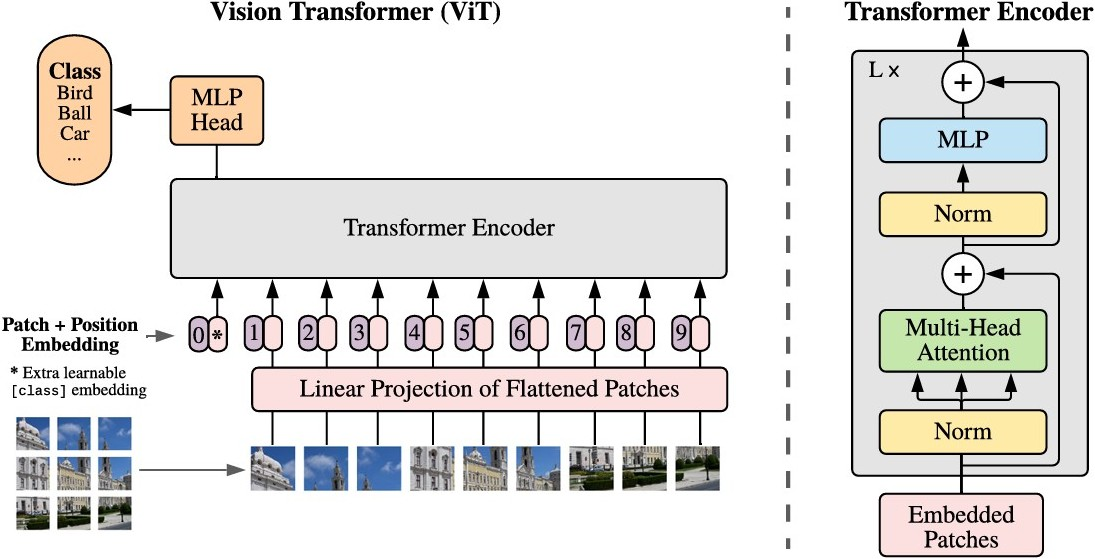
\includegraphics[width=0.9\linewidth]{graphics/ViT-architecture.jpg}
      \caption[Schematischer Aufbau einer Vision Transformer Architektur]{Schematischer Aufbau einer Vision Transformer Architektur\footnotemark }
      \label{fig:vit}
\end{figure}
\footnotetext{Entnommen aus: \cite[S. 3]{dosovitskiy_image_2020}}

Architektonisch wird wie in Abbildung \ref{fig:vit} zu sehen ist bei einem \ac{ViT} das Eingabebild in mehrere Patches zerlegt und diese mittels trainierbarer linearer Projektion in einen Vektor umgewandelt. Dieser Vektor wird um eine Positionsinformation ergänzt und anschließend an den \textit{Transformer Encoder} übergegeben\footnote{Vgl. \cite[3]{dosovitskiy_image_2020}} Durch den Einsatz von \textit{Multi-Head Self-Attention} kann dieser \textit{Encoder} globale Abhängigkeiten zwischen allen Patches modellieren und somit Kontext effektiv bewahren. Durch ein neuronales Netz findet anschließend eine Klassifikation statt.\footnote{Vgl. \cite[3]{dosovitskiy_image_2020}} Der \textit{Transformer Encoder} ist dabei nicht spezifisch auf Bilddaten ausgelegt, sondern könnte auch für andere Sequenzdaten, wie \textit{Text-Embeddings}, verwendet werden.\footnote{Vgl. \cite[3]{dosovitskiy_image_2020}}

Beispielsweise können \acfp{ViT} im Gegensatz zu \acp{CNN} besser globale Bildmerkmale sowie Zusammenhänge verschiedener Elemente bewahren\footnote{Vgl. \cite[S. 206]{berroukham_vision_2023}}, wodurch sie in der Praxis schon erfolgreich Anwendung finden und in Fällen, wie im medizinischen Umfeld zur Erkennung von bestimmten Krankheiten, \acp{CNN} übertreffen.\footnote{Vgl. \cite[S. 208]{berroukham_vision_2023}}

Trotz ihrer Erfolge sind \acp{ViT} mit einer Reihe technischer Herausforderungen verbunden. Hierzu gehören neben höheren Rechenkosten durch eine große Anzahl an Parametern auch die Notwendigkeit von größeren Datensätzen, da diese ansonsten oftmals schlechter als \ac{CNN}-Architekturen abschneiden.\footnote{Vgl. \cite[8]{jamil_comprehensive_2022}} \acp{ViT} sind außerdem stärker davon abhängig, dass Trainingsdaten nicht in schlechter Qualität oder verzerrt vorliegen.\footnote{Vgl. \cite[209]{berroukham_vision_2023}} Die Arbeit von \cite{hutten_vision_2022} zeigt allerdings, dass auch solche Herausforderungen mit geeigneten Transformer-Architekturen adressiert werden können. In ihrer Arbeit wurden verschiedene Modelle zur Anwendbarkeit von \acp{ViT} in der industriellen Inspektion am Beispiel von Güterwagen getestet. Dabei wurden Transformer-Architekturen mit \ac{CNN}-basierten Ansätzen verglichen, indem sie auf dem gleichen, kleinen Datensatz trainiert und evaluiert wurden. Die Transfomer-Modelle erzielten hierbei bessere Ergebnisse als \acp{CNN}, ohne signifikante Unterschiede in der Trainingsgeschwindigkeit aufzuweisen, was die Potenziale von \acp{ViT} auch in datenlimitierten industriellen Umgebungen deutlich unterstreicht.\footnote{Vgl. \cite{hutten_vision_2022}}

%\textcolor{red}{Ich bin mir wegen dem Umfang unsicher, deswegen wurde folgendes Paper nicht aufgenommen, könnte aber intererssant sein: es geht auf eine Hybride Varianten ein und stellt ebenfalls Unterschiede und Vor-/Nachteile von \acp{CNN} bzw. \acp{ViT} heraus. Es enthält auch, wer erste Entwicklungen bei Text- und Bild-Transformern entwickelt hatte: https://doi.org/10.48550/arXiv.2305.09880}

%\textcolor{red}{Zusätzlich noch VLMs nennen?}

%\textcolor{red}{Sollte noch auf Risiken oder Probleme eingangen werden beim Einsatz von KI? z.B. das Problem der Erklärbarkeit, insbesondere in Bezug auf die Nutzung von digitalen Zwillingen im Bereich Predictive Maintenance oder der Fehlerkennung/-klassifizierung}


\section{Fehlererkennung und -klassifikation in der Fertigung}

Die Fehlererkennung und -klassifikation (engl. \textit{\ac{FDD}}) ist keine neue Thematik, sondern wird bereits seit Anfang der 70er Jahre untersucht.\footnote{Vgl. \cite[S. 4]{mercorelli_recent_2024}} Aufgrund der neuen vielversprechenden technischen Entwicklungen, insbesondere im Bereich des \ac{DL}, wird diese Thematik jedoch immer relevanter, insbesondere mit Fokus auf die Implementierung von \ac{KI}-Technologien zur Unterstützung dieses Prozesses.\footnote{Vgl. \cite[S. 1]{seid_ahmed_advances_2025}} Neben der reinen Fehlervermeidung bietet \ac{FDD} durch ein schnelles Erkennen und korrektes Reagieren auf Fehler erhebliche wirtschaftliche Vorteile, wie die Reduktion von Prozesskosten sowie die Steigerung der Produktivität und Qualität in der Fertigung.\footnote{Vgl. \cite[S. 4]{seid_ahmed_advances_2025}}

\subsection{Begriffsdefinition und -abgrenzung}
Die Fehlererkennung (engl. \textit{Fault Detection}) konzentriert sich darauf, festzustellen, ob ein Fehler oder eine Anomalie vorliegt. Anschließend zielt die Fehlerdiagnose (engl. \textit{Fault Diagnostics}) darauf ab, den Fehler in Kategorien bekannter Fehler einzuordnen und somit zu klassifizieren.\footnote{Vgl. \cite[S. 442]{wu_transformer-based_2023}} Dazu gehört außerdem möglichst viel über den Fehler und dessen Ursprung in Erfahrung zu bringen, weshalb man die Fehlerdiagnose üblicherweise als einen mehrstufigen Prozess betrachten kann, welcher die Erkennung, Isolation, Identifizierung sowieso Klassifizierung und Bewertung umfasst.\footnote{Vgl. \cite[S. 12]{mercorelli_recent_2024}; \cite[S. 16]{seid_ahmed_advances_2025}}

\subsection[Kategorien von Fault Detection and Diagnostics (FDD) Methoden]{Kategorien von \ac{FDD} Methoden}
Es wurden viele verschiedene \ac{FDD}-Methoden entwickelt, welche sich in 3 Gruppen einteilen lassen: \textit{Data-driven}, \textit{Model-based} und \textit{Knowledge-based} Methoden. Im Folgenden sollen diese Methoden unterschieden werden\footnote{Vgl. \cite[S. 4]{seid_ahmed_advances_2025}}

\textbf{Datengetriebene Methoden (Data-driven)} 

Datengetriebene Methoden nutzen historische Daten, um durch statistische Techniken oder \textit{Machine Learning}-Algorithmen charakteristische Muster und Abweichungen zu erkennen und dadurch Anomalien und Fehler erkennen und klassifizieren zu können. Diese Verfahren sind deutlich anpassungsfähiger als andere Methoden und können auch komplexe Prozesse überwachen. Sie sind insbesondere dann nützlich, wenn umfangreiche Daten bereits vorliegen. Allerdings zeigt sich hier auch der Nachteil solcher Verfahren, da große, repräsentative Datensätze für das Training solcher Modelle erforderlich sind.\footnote{Vgl. \cite[S. 16 ff.]{mercorelli_recent_2024}}

\textbf{Modellbasierte Methoden (Model-based)}

Diese Verfahren stützen sich auf ein physikalisches oder mathematisches Modell des Systems, aufgrund welchem das erwartete Verhalten berechnet werden kann. Eine Abweichung des tatsächlichen vom erwarteten Verhalten weist auf einen potenziellen Fehler hin und kann zur dessen Identifikation und Klassifikation herangezogen werden. Die größten Herausforderungen sind hierbei der Rechenaufwand sowie das nötige Verständnis über das System. Sind diese Faktoren jedoch gegeben, kann diese Methode sehr präzise sein.\footnote{Vgl. \cite[S. 21 ff.]{mercorelli_recent_2024}}

\textbf{Wissensbasierte Methoden (Knowledge-based)} 

Wissensbasierte Verfahren basieren auf kodiertem Expertenwissen und sind dadurch besonders nützlich, wenn fundiertes Fachwissen vorliegt. Ein wesentlicher Vorteil liegt neben einer hohen Verarbeitungsgeschwindigkeit in der Nachvollziehbarkeit der Entscheidungen des Systems. Bei bislang unbekannten Fehlern sowie unvollständigem oder falschem Expertenwissen stoßen diese Methoden jedoch an ihre Grenzen.\footnote{Vgl. \cite[S. 22 f.]{mercorelli_recent_2024}}

\textbf{Hybride Methoden}

Es existieren außerdem hybride-Verfahren, bei welchen Elemente aus \textit{model-based}, \textit{data-based} und \textit{knowledge-based} Ansätzen kombiniert werden, um jeweilige Stärken zu nutzen und bestehende Schwächen auszugleichen. Dadurch wird das System robuster und flexibler, jedoch kann hier die Integration der verschiedenen Methoden ineinander eine Herausforderung darstellen.\footnote{Vgl. \cite[S. 22 f.]{mercorelli_recent_2024}}

\subsection{Aktuelle Trends}
Aktuelle Trends befinden sich zurzeit vor allem im Bereich der künstlichen Intelligenz. \ac{DL} steht im Bereich der \ac{FDD} immer mehr im Mittelpunkt, um Merkmale aus Rohdaten automatisiert zu extrahieren und die Fehlererkennung und Diagnose voranzutreiben.\footnote{Vgl. \cite[S. 5991]{wen_new_2018}}
Zu den populärsten Anwendungen von \ac{DL} in der \ac{FDD} zählen immer noch \acp{CNN}, um Bilddaten zu analysieren und Degradationsmuster aus Sensordaten zu extrahieren.\footnote{Vgl. \cite{wu_transformer-based_2023}; \cite[S.  5991]{wen_new_2018}} Allerdings zeigt die Forschung aktuell, wie bereits in \ref{sec:ki_modelle_bildverarbeitung} erläutert, ein steigendes Interesse an der Nutzung von \acp{ViT} in der Fertigungsindustrie, welche die Leistung von \acp{CNN} übertreffen können. \acp{ViT} bieten unter anderem durch ihr Aufmerksamkeitsmechanismen ein großes Potenzial beim Umgang mit \ac{FDD}-Daten.\footnote{Vgl. \cite[S. 440]{wu_transformer-based_2023}}Ein wesentlicher Vorteil bei der Nutzung von Transformern besteht zudem in der Möglichkeit zur Neuheitserkennung (engl. \textit{Novel Detection}). Das bedeutet, dass das Modell neue oder unbekannte Fehler identifizieren kann, welche vorher noch nicht beobachtet wurden.

\subsection{Herausforderungen und Forschungsbedarf}
Trotz der erzielten Fortschritte bestehen mehrere zentrale Herausforderungen. Zu diesen gehören wie schon in \ref{sec:synthetische_daten_section} beschrieben, die Notwendigkeit von großen Mengen an annotierten, vielfältigen Daten, was insbesondere im Fertigungsbereich eine aktuelle Problematik darstellt und durch die Generierung von synthetischen Daten in dieser Arbeit adressiert werden soll. Des weiteren stellt die Komplexität und Interpretierbarkeit von Modellen eine aktuelle Herausforderung dar. \ac{DL} Modelle werden oftmals als "Black Boxes" betrachtet, bei welchen dessen Entscheidungslogik nur schwer nachvollzogen werden kann.\footnote{Vgl. \cite[S. 10]{chai_deep_2021}} Eine weitere Herausforderung stellt die Generalisierung solcher Modelle dar. Treten neue Fehler auf, welche beim Training nicht vorhanden waren, werden diese vom Modell inkorrekt klassifiziert.\footnote{Vgl. \cite[S. 440]{wu_transformer-based_2023}}
Aus der Literatur lässt sich damit ein dringender Bedarf an leistungsfähigen \ac{FDD}-Methoden ableiten, insbesondere für eine zuverlässige und echtzeitfähige Fehlerdiagnose in großskaligen Produktionssystemen, sodass weitere Forschung und Entwicklung in diesem Bereich unerlässlich ist.\footnote{Vgl. \cite[S. 4]{seid_ahmed_advances_2025}; \cite[S. 442]{wu_transformer-based_2023}}


\section{Remote Monitoring}

\subsection{Begriffsabgrenzung: Remote Services, Remote Operations, Remote Monitoring}
Der Begriff Remote Services dient als Sammelbegriff für verschiedene Formen der ortsunabhängigen Unterstützung, unter welchen unter anderem die Serviceformen Remote Repair, Remote Maintenance und Remote Operations fallen.\footnote{Vgl. \cite[S. 5]{holtbrugge_remote_2007}}
Unter dem Begriff der Remote Operations versteht man die aktive Fernüberwachung, Ferndiagnose sowie den Fernbetrieb einer Anlage. Remote Monitoring bezeichnet die Fernüberwachung und -diagnose und kann somit als Teil der Remote Operations eingeordnet werden.\footnote{\cite[S. 592 f.]{vogel-heuser_remote_2024}}

\iffalse
\subsection{Differenzierungen von Remote Operations}
Die Namur-Empfehlung NE 161 differenziert Remote Operations in drei Kategorien, welche sich in ihrem Grad der Autonomie unterscheiden:
\begin{itemize}
    \item \textbf{Kategorie 1:} Anlagen werden überwiegend vor Ort gesteuert und überwacht\footnote{\cite[S. 593]{vogel-heuser_remote_2024}}
    \item \textbf{Kategorie 2:} Anlagen können für einen begrenzten Zeitraum aus der Ferne betrieben werden,  beispielsweise in Nacht- oder Wochenendschichten, wodurch nicht jederzeit Personal vor Ort erforderlich ist. Es werden allerdings weiterhin Tätigkeiten vor Ort durchgeführt.\footnote{\cite[S. 593]{vogel-heuser_remote_2024}}
    \item \textbf{Kategorie 3:} Vollständig fernbediente Anlagen, bei denen nur in Ausnahmefällen Personal herangezogen wird. Im Regelfall befindet sich kein Personal in der Anlage.\footnote{\cite[S. 593]{vogel-heuser_remote_2024}}  
\end{itemize}

Die NAMUR-Empfehlung unterscheidet zudem in 3 aufeinander aufbauenden Ebenen: Fernüberwachung, Ferndiagnose und Fernsteuerung:
\begin{itemize}
    \item \textbf{Fernüberwachung:} Kontinuierliche Beobachtung der Anlage, beispielsweise durch KPIs, wobei jedoch keine Diagnose von Fehlern stattfindet.\footnote{\cite[S. 593]{vogel-heuser_remote_2024}}
    \item \textbf{Ferndiagnose:} Baut auf der Fernüberwachung auf und erlaubt neben der Überwachung der Anlage auch eine Analyse und Bewertung der Daten, wobei diese Ebene keine Eingriffe in den tatsächlichen Prozess erlaubt.\footnote{\cite[S. 593]{vogel-heuser_remote_2024}}
    \item \textbf{Fernsteuerung:} Erst auf dieser Ebene sind auch direkte Eingriffe in die Anlage und deren Prozess möglich.\footnote{\cite[S. 593]{vogel-heuser_remote_2024}}
\end{itemize}

Remote Monitoring lässt sich folglich in Kategorie 2 und der Ebene der Fernüberwachung einordnen, da weiterhin Personal vor Ort vorhanden sein muss und keine Eingriffe in den Prozess nicht umfasst sind, sondern ausschließlich die Überwachung und Analyse der erfassten Daten. Remote Operations hingegen kann je nach Ausprägung den Kategorien 2 bis 3 und der Ebene der Fernsteuerung zugeordnet werden.
\fi

\subsection{Remote Monitoring in der Fertigung}
Durch Remote Monitoring wird eine kontinuierliche Überwachung und Analyse der Fertigungsanlage gewährleistet, wodurch Fehlerfälle schneller erkannt und klassifiziert werden können. Dies erleichtert die Fehlerbehebung in den nachfolgenden Schritten, wodurch die Effizienz und Auslastung der Anlage erhöht als auch Kosten eingespart werden können.\footnote{Vgl. \cite[S. 110]{holtbrugge_remote_2007}} Darüber hinaus schafft Remote Monitoring die Grundlage für ferngesteuerten Reparaturen und Instandhaltungen im Rahmen von Remote Operations, wodurch Kosten reduziert werden und das Personal effizienter ausgelastet werden kann.\footnote{Vgl. \cite[S. 5, 110]{holtbrugge_remote_2007}} Remote Services gewinnen zunehmend an Bedeutung, weshalb dieses Themengebiet einen wichtigen Forschungszweig darstellt.\footnote{Vgl. \cite[S. 5]{holtbrugge_remote_2007}}
Auch bei TRUMPF kommt Remote Monitoring zum Einsatz, um Fehler bei Stillständen von Maschinen aus der Ferne identifizieren zu können, um diese anschließend per Fernzugriff zu entstören.

\subsection{Voraussetzungen für Remote Monitoring}
Für die Umsetzung eines effektiven Remote Monitoring Systems ist es nötig, die menschlichen Sinne und menschliche Intelligenz nachzubilden, um Zustände korrekt wahrzunehmen und zu interpretieren.\footnote{Vgl. \cite[S. 596]{vogel-heuser_remote_2024}} Zur Nachbildung der menschlichen Sinne kommen je nach Anwendungsfall verschiedene Sensoren, wie beispielsweise Kameras, Mikrofone, Temperatur- oder Gassensoren, zum Einsatz.\footnote{Vgl. \cite[S. 596 f.]{vogel-heuser_remote_2024}} Um menschliche Intelligenz nachzubilden eignen sich verschiedene Methoden der künstlichen Intelligenz. Die Auswahl des geeigneten Algorithmus richtet sich hierbei ebenfalls nach den spezifischen Anforderungen des Anwendungsfalls.\cite[S. 597]{vogel-heuser_remote_2024}


\section[Evaluationsmethoden für Computer Vision-Modelle]{Evaluationsmethoden für \ac{CV}-Modelle}

\subsection{Grundlagen der Modellevaluation}
\ac{KI} Modelle zu evaluieren ist entscheidend, um ihre Leistung, Zuverlässigkeit und Eignung für den jeweiligen Anwendungsfall beurteilen und verschiedene Modelle vergleichen zu können. Sie ermöglicht zudem den Vergleich unterschiedlicher Modellarchitekturen, wie beispielsweise \acp{CNN} und \acp{ViT}.\footnote{Vgl. \cite[S. 105281]{ali_adversarial_2024}}

Ziel der Modellevaluation ist es, die Leistungsfähigkeit eines Modells quantitativ zu erfassen. Neben der reinen Genauigkeit (engl. \textit{Accuracy}) spielen außerdem weitere Kennzahlen wie Präzision (engl. \textit{Precision}), Sensitivität (engl. \textit{Recall}) und der harmonische Mittelwert dieser beiden, der \textit{\(F1\)-Score}, eine zentrale Rolle, insbesondere bei unausgeglichenen Datensätzen\footnote{Vgl. \cite[S. 65240]{arslanoglu_vision_2025}}. Des weiteren ist die Robustheit von Modellen, also die Fähigkeit, unter variierenden Eingabebedingungen (z.B. Rauschen, Helligkeit, Rotation, Bildqualität, geometrische Unterschiede) konsistente Ergebnisse zu liefern, ebenfalls entscheidend.\footnote{Vgl. \cite[S. 65234]{arslanoglu_vision_2025}} Diese kann durch Tests unter veränderten Bedingungen ermittelt werden.\footnote{Vgl. \cite[S. 323]{zhang_computer_2023}}

\subsection{Zentrale Evaluationsmetriken für die Objekterkennung}

Während die Genauigkeit angibt, welcher Anteil aller Vorhersagen korrekt ist, misst die Präzision (\(P\)) den Anteil der als positiv klassifizierten Vorhersagen, welche auch korrekterweise positiv (engl. \textit{\ac{TP}}) sind.\footnote{Vgl. \cite[S. 65240]{arslanoglu_vision_2025}}
\[
P = \frac{\text{\acs{TP}}}{\text{\acs{TP}} + \text{\acs{FP}}}
\]
Die Sensitivität (\(R\)) hingegen misst den Anteil der korrekt erkannten positiven Instanzen an allen tatsächlich positiven Instanzen, also \acf{TP} + \ac{FN}.\footnote{Vgl. \cite[S. 65240]{arslanoglu_vision_2025}} 
\[
R = \frac{\acs{TP}}{\acs{TP} + \acs{FN}}
\]

Für Objekterkennungsaufgaben werden typischerweise spezifische Metriken eingesetzt, die neben der Klassifikationsleistung auch die Genauigkeit der Lokalisierung berücksichtigen, wie etwa die \ac{AP} oder die daraus abgeleitete \ac{mAP}.\footnote{Vgl. \cite[S. 94272]{khanam_comprehensive_2024}} Grundlage der Bewertung, ob eine Detektion als korrekt gilt, ist die \ac{IoU}, welche den Überlappungsgrad zwischen vorhergesagter und tatsächlicher \textit{Bounding Box} misst.\footnote{Vgl. \cite[S. 94272]{khanam_comprehensive_2024}} Ein gängiger Schwellenwert hierfür ist 0.5, wonach die Detektion als erfolgreich klassifiziert wird, wenn die vorhergesagte und tatsächliche \textit{Bounding Box} um mindestens 50\% übereinstimmen.\footnote{Vgl. \cite[S. 94272]{khanam_comprehensive_2024}}

Die \ac{AP} entspricht der Fläche unter der Precision–Recall-Kurve bei einem festgelegten \ac{IoU}.-Schwellenwert (z.\,B. 0.5. für \ac{AP}50).\footnote{Vgl. \cite[13]{zaripov_creation_2025}}

\[
\acs{AP} = \int_0^1 p(r) \, dr
\]

Die \ac{mAP} ist der Mittelwert der \ac{AP}-Werte über alle Klassen.\footnote{Vgl. \cite[14]{zaripov_creation_2025}} Je nach Evaluationsprotokoll kann zudem über mehrere \ac{IoU}-Schwellenwerte gemittelt werden. In der Praxis wird häufig \ac{mAP}50 verwendet, d.\,h. der Mittelwert der \ac{AP} über alle Klassen bei \ac{IoU}-Schwelle 0.5.\footnote{Vgl. \cite[S. 13 f.]{zaripov_creation_2025}}

In diesem Zusammenhang wird häufig der \ac{mAP}50 verwendet, welcher die \ac{mAP}-Metrik mit Verwendung der \ac{IoU}-Schwelle 0.5 berechnet.\footnote{Vgl. \cite[S. 13]{zaripov_creation_2025}}


\subsection{Vergleich und Auswahl von Metriken}

Die Auswahl geeigneter Evaluationsmetriken hängt maßgeblich von den Datencharakteristika, der Aufgabenstellung und den Prioritäten des Anwendungsfalls ab. In der Objekterkennung hat sich insbesondere die Mean Average Precision (\ac{mAP}) etabliert, da sie sowohl Klassifikations- als auch Lokalisierungsfehler berücksichtigt und damit ein differenziertes Bild der Modellleistung liefert.\footnote{Vgl. \cite[S. 65240]{arslanoglu_vision_2025}; \cite[S. 94272]{khanam_comprehensive_2024}} 

Insbesondere in sicherheitskritischen Bereichen ist es darüber hinaus sinnvoll, die Robustheit eines Modells gegenüber veränderten Eingabebedingungen mit zu berücksichtigen, um ein umfassenderes Bewertungsbild zu erhalten.\footnote{Vgl. \cite[S. 65234]{arslanoglu_vision_2025}; \cite[S. 105282]{ali_adversarial_2024}} Häufig empfiehlt sich daher eine kombinierte Evaluation, bei der mehrere Kennzahlen einbezogen werden, um unterschiedliche Leistungsaspekte des Modells abzudecken.

\chapter[Zielspezifikation und Darlegung des Forschungsdesigns]{Zielspezifikation und Darlegung des Forschungsdesigns\footnote{Sprachlich geglättet durch ChatGPT-5}}
\label{chapter:Ziel_und_Forschungsdesign}

\section{Zielsetzung}\label{sec:zielsetzung}
Ziel dieser Arbeit ist die prototypische Entwicklung und Evaluation eines IT-Artefakts in Form einer Datenpipeline zur Generierung synthetischer Bilddaten aus einem digitalen Modell einer Laserschneidmaschine in einer Simulationsumgebung. Die Pipeline soll automatisiert umfangreiche und qualitativ hochwertige Bilddatensätze erzeugen, die spezifische Fehlerzustände der Maschine abbilden. Dabei stehen die Reproduzierbarkeit des Prozesses, die Flexibilität durch Parametrisierung sowie die einfache Erweiterbarkeit um zusätzliche Fehlerzustände im Vordergrund.

Zur Validierung der Pipeline werden die erzeugten Daten exemplarisch für das Training und die Evaluation von \ac{KI}-Modellen eingesetzt. Diese Modelle bilden nicht den Hauptfokus der Arbeit, sondern dienen als Mittel, um die Eignung und Konsistenz der generierten synthetischen Daten nachzuweisen. Die Evaluation der Modelle erfolgt dabei sowohl auf synthetischen als auch realen Bilddaten. Die Arbeit versteht sich somit als \textit{Proof-of-Concept}, der die Machbarkeit und das Potenzial pipelinebasierter Datengenerierung für die \ac{KI}-gestützte Fehlererkennung in der Fertigungsindustrie aufzeigt. Erzielte Ergebnisse sollen dabei auch auf andere Domänen übertragbar sein, da der Mangel an ausreichenden und umfassenden Bilddaten für solche Anwendungen nicht ausschließlich in der Fertigungsindustrie eine Problematik darstellt.\footnote{Vgl. \cite[2]{bai_bridging_2023}}

Exemplarisch wird die Pipeline in einem konkreten Anwendungsfall eingesetzt, bei welchem erkannt werden soll, ob ein ausgeschnittenes Teil während des Betriebs einer Laserschneidmaschine noch im Blech vorhanden ist. Mit einer solchen Information kann nachgelagerten Prozessen der konkrete Fehlerfall klassifiziert und im Idealfall autonom behoben werden. Dieser Anwendungsfall dient als Demonstrator, um die Funktionsfähigkeit und den praktischen Nutzen der Pipeline im Rahmen eines \textit{Proof-of-Concepts} zu veranschaulichen.


\section{Forschungsmethodik}\label{sec:forschungsmethodik}
Zur Erreichung der in Abschnitt \ref{sec:zielsetzung} beschriebenen Zielsetzung wird das \ac{DSR}-Paradigma angewendet. Bei \ac{DSR} handelt es sich um einen anerkannten Forschungsansatz in Informationssystemen, der darauf abzielt, durch die Entwicklung und Evaluation innovativer Artefakte, Probleme in der Praxis zu lösen und gleichzeitig einen Beitrag zur wissenschaftlichen Wissensbasis zu leisten.\footnote{Vgl. \cite[S.337]{the_australian_national_university_positioning_2013}}
Im Rahmen von \ac{DSR} werden Artefakte, wie z.B. Systeme, Methoden oder Modelle entworfen und iterativ in einem \textit{Build-and-Evaluate}-Zyklus weiterentwickelt, um ihre Eignung zur Problemlösung zu überprüfen und zu verbessern.\footnote{Vgl. \cite[78]{hevner_design_2004}} Dieser Prozess umfasst die Identifikation des Problems, die Definition von Anforderungen, die Entwicklung eines Artefakts sowie dessen Demonstration, Evaluation und Kommunikation. \footnote{Vgl. \cite{peffers_design_2007}}

Das in dieser Arbeit entwickelte Artefakt besteht aus einer Pipeline zur Generierung synthetischer Bilddaten, die auf einem digitalen Modell in einer Simulationsumgebung basiert. Das Ziel ist es, die Datengrundlage für \ac{KI}-Modelle zur Fehlererkennung im Fertigungsbereich zu verbessern, insbesondere in Hinblick auf Fortschritte im Bereich des Remote Monitoring. Bereits in Abschnitt \ref{sec:synthetische_daten_section} genannte Probleme, wie Kosten- und Zeitaufwand sowie der \textit{Domain Gap} sollen durch dieses Artefakt konzeptionell adressiert werden. 

Nach der Definition der Problemstellung und Zielsetzung sowie Erläuterung zentraler theoretischer Grundlagen wird das Artefakt entworfen, implementiert und in einem Demonstrator angewendet. Anschließend erfolgt die Evaluation auf synthetischen und realen Bilddaten sowie eine kritische Reflexion der Ergebnisse.

Die Wahl des \ac{DSR}-Paradigmas ist für den vorliegenden Use Case besonders geeignet, da es sich um ein praxisnahes Problemfeld handelt. Die genannten Herausforderungen werden durch \ac{DSR} adressiert, indem ein Artefakt in Form einer synthetischen Datenpipeline entwickelt und evaluiert wird. Es wird dadurch einerseits ein praktischer Nutzen erzielt,\footnote{Vgl. \cite[341]{the_australian_national_university_positioning_2013}} indem der Umfang und die Qualität der Daten für das Training von \ac{KI}-Modellen verbessert werden. Andererseits wird die Effektivität synthetischer Daten empirisch untersucht und insbesondere im Hinblick auf den \textit{Domain Gap} reflektiert, wodurch ein wissenschaftlicher Beitrag im Sinne des \ac{DSR} geleistet wird.\footnote{Vgl. \cite[342]{the_australian_national_university_positioning_2013}}

Die vorliegende Arbeit lässt sich im Sinne des \textit{\ac{DSR} Knowledge Contribution Framework} als \textit{Improvement} einordnen.\footnote{Vgl. \cite[S. 345 f.]{the_australian_national_university_positioning_2013}} Zwar sind Probleme wie Datenknappheit, Zeitaufwand und \textit{Domain Gap} bei synthetischen Daten bereits bekannt, jedoch stellt die in dieser Arbeit entwickelte Datenpipeline eine neue und domänenspezifische Lösung für das Training von \textit{KI}-Modellen zur Fehlererkennung dar. Damit trägt die Arbeit durch die Weiterentwicklung bestehender Konzepte zur verbesserten Lösung eines etablierten Problems bei.


\section{Darlegung des Forschungsdesigns}\label{sec:forschungsdesign}

\subsection{Artefaktdefinition}\label{subsec:artefaktdefinition}

Bei dem entwickelten Artefakt handelt es sich um eine Datenpipeline zur Generierung umfangreicher synthetischer Bilddaten und zum Training von \ac{KI}-Modellen auf diesen zur Fehlererkennung in der Fertigungsindustrie. Hierzu soll ein Fertigungsprozess simuliert werden, welcher mit realitätsnah konfigurierten Kameras erfasst werden soll. Um die Generalisierungsfähigkeit des Modells zu erhöhen soll im Rahmen der Datengenerierung auf \textit{Domain Randomization} zurückgegriffen werden.\footnote{Vgl. \cite[4427]{fulir_synthetic_2023}} Dabei werden verschiedene Parameter, wie beispielsweise Lichtverhältnisse, das bearbeitete Material oder Kameraperspektiven, zufällig verändert, um das Modell robuster gegen äußere Einflüsse zu gestalten und die Gefahr von \textit{Overfitting} zu reduzieren.\footnote{Vgl. \cite[263]{urgo_monitoring_2024}; \cite[4427]{fulir_synthetic_2023}} Auch Elemente des Produktionsprozesses, wie verschiedene Fehlersituationen oder Störobjekte werden zufällig verändert, um die Übertragbarkeit auf reale Anwendungsfälle zu verbessern.\footnote{Vgl. \cite[767]{monnet_investigating_2024}}
Zentral ist dabei, dass die Pipeline flexibel und erweiterbar gestaltet ist, sodass problemlos weitere Fehlerfälle integriert sowie Qualität und Umfang der generierten Daten angepasst werden können. Bei der Umsetzung und Implementierung wird zudem auf eine systematische und detaillierte Dokumentation geachtet, um die Reproduzierbarkeit der Experimente sicherzustellen.

Die Bilddaten sollen aus dem Simulationsprogramm exportiert werden und für das Training verschiedener \ac{KI}-Modelle und Architekturen Verwendung finden. Die verschiedenen Modelle werden aufgrund etablierter Metriken verglichen und bezüglich ihrer Leistung und Generalisierungsfähigkeit evaluiert. Essenziell ist dabei, dass die Trainings- und Testvoraussetzungen für alle Modelle und Architekturen möglichst identisch sind, um eine bestmögliche Vergleichbarkeit zu gewährleisten. Wie schon in Abschnitt \ref{sec:zielsetzung} beschrieben steht allerdings die Validierung der generierten Daten im Vordergrund und nicht die Entwicklung eines optimalen Modells für den Anwendungsfall.


\subsection{Vorgehensweise}
Das methodische Vorgehen in dieser Arbeit orientiert sich wie bereits in Abschnitt \ref{sec:forschungsmethodik} beschrieben am \ac{DSR}-Paradigma. Zunächst erfolgt die Konzeption des Artefakts in Form einer Datenpipeline. Anschließend wird diese Pipeline für die Generierung synthetischer Bilddaten eingesetzt, wobei mittels \textit{Domain Randomization} verschiedene Parameter zufällig variiert werden. Pixelgenaue Annotationen der synthetischen Bilddaten werden automatisch durch die Simulationsumgebung hinzugefügt und gemeinsam mit den Bilddaten gespeichert. Die Annotationen werden in ein für das Training des Modells geeignetes Format überführt und anschließend zusammen mit den Bilddaten in ein Trainings-, Validierungs- und Testdatensatz unterteilt. Diese Datensätze werden für das Training verschiedener \textit{KI}-Modelle sowie deren anschließende Evaluation verwendet. Während des Trainings kommt zusätzlich eine weitere Variation und Vergrößerung des Datensatzes durch Datenaugmentation (engl. \textit{Data Augmentation}) zum Einsatz. Unter Datenaugmentation wird die gezielte Variation vorhandener Trainingsbilder, beispielsweise durch Anpassung von Belichtung, Sättigung, Farben, Zoom oder Bildkomposition verstanden. Ziel ist es, den Datensatz künstlich zu vergrößern und die Generalisierungsfähigkeit des Modells, insbesondere bei Limitationen durch kleine Datensätze, zu verbessern.\footnote{Vgl. \cite[S. 2 f.]{shorten_survey_2019}; \cite{ultralytics_yolo-datenerweiterung_nodate}} Nach dem Training der \textit{KI}-Modelle erfolgt deren Evaluation auf Basis der in Abschnitt \ref{subsec:evaluationsdesign} definierten Metriken. Die erzielten Ergebnisse dienen in erster Linie als Validierung der generierten synthetischen Daten und sollen Aufschluss darüber geben, inwiefern diese für industrielle Anwendungen geeignet sind. Darüber hinaus werden die Erkenntnisse hinsichtlich des \textit{Domain Gaps} reflektiert. Im Sinne des \ac{DSR} ist es vorgesehen, die gewonnenen Erkenntnisse zu nutzen, um das Artefakt iterativ weiterzuentwickeln.

\subsection{Datengrundlage}
Die Datengrundlage der Experimente bilden überwiegend synthetische Bilddaten, welche mithilfe eines digitalen Modells in einer Simulationsumgebung generiert werden. Dabei werden Zustände und Fehlerfälle des Fertigungsprozesses simuliert und wie bereits in Abschnitt \ref{subsec:artefaktdefinition} erläutert, verschiedene Parameter wie unter anderem Lichtverhältnisse, Materialien und die Kameraperspektive durch \textit{Domain Randomization} variiert.

Ergänzend zu den synthetischen Daten wird eine kleinere Menge an realen Bilddaten herangezogen, welche als Testdaten zur Evaluation der trainierten Modelle dient. Dadurch soll überprüft werden, inwieweit Modelle, welche ausschließlich auf synthetischen Daten trainiert wurden, in industriellen Anwendungen leistungsfähig sind und welche Schwierigkeiten bei der Übertragbarkeit bestehen.

Als Basis für die Generierung der Bilddaten dienen \ac{USD}-Modelle, welche primär verschiedene Zustände von einem Blech im Schneidprozess abbilden. Die zugrunde liegenden 3D-Modelle wurden durch die TRUMPF SE + Co. KG bereitgestellt und in die Simulationsumgebung übertragen.


\subsection{Evaluationsdesign}\label{subsec:evaluationsdesign}
Die Evaluation des entwickelten Artefakts erfolgt anhand etablierter Metriken aus dem Bereich der Objekterkennung. Insbesondere die Kennzahlen \acf{AP} und \acf{mAP}, die auf der \acf{IoU} basieren, sind für die Objekterkennung und auch für diesen Anwendungsfall zentral.\footnote{Vgl. \cite[94272]{khanam_comprehensive_2024}} Verwendet werden dabei insbesondere die Varianten \ac{mAP}@50, bei der die \ac{mAP} bei einer \ac{IoU}-Schwelle von 0,5 berechnet wird, sowie \ac{mAP}@[.5:.95], bei der die \ac{AP}-Werte über die \ac{IoU}-Schwellen 0,5 bis 0,95 berechnet und gemittelt werden. Die Metrik \ac{mAP}@[.5:.95] erfordert daher ein höheres Maß an Präzision, wodurch eine genauere Analyse der Lokalisierungsgenauigkeit ermöglicht wird.\footnote{Vgl. \cite[S. 94272 f.]{khanam_comprehensive_2024}}

Vor der Berechnung dieser Kennzahlen werden die Modellvorhersagen einem \acf{NMS} unterzogen. \ac{NMS} ist ein Verfahren, bei dem überlappende Bounding Boxes entfernt werden, um Mehrfacherkennungen desselben Objekts zu vermeiden und die Vergleichbarkeit der Ergebnisse zu gewährleisten.\footnote{Vgl. \cite[S. 4508 f.]{hosang_learning_2017}}

Die Vergleichbarkeit der Ergebnisse zwischen verschiedenen Architekturen und Modellvarianten wird durch konsistente Rahmenbedingungen sichergestellt. Dazu zählen unter anderem identische Datensätze, einheitliche Trainings-, Validierungs- und Test-Splits sowie identische Hyperparameter bei Modellvarianten der gleichen Architektur. Auf diese Weise kann gewährleistet werden, dass Unterschiede in der Modellleistung auf die Datengrundlage oder gewählte Trainingsstrategie zurückzuführen sind und nicht auf methodische Inkonsistenzen.


\subsection{Reproduzierbarkeit und Validität}
Um die Experimente und deren Ergebnisse bestmöglich reproduzieren zu können, werden sämtliche Parameter der Datengenerierung sowie des Modelltrainings systematisch dokumentiert. Dazu zählen beispielsweise die Konfiguration von Licht- und Materialverhältnisse sowie von Kamerapositionen im Rahmen der \textit{Domain-Randomization}, die verwendeten Software- und Modellversionen sowie die Hyperparameter des Modelltrainings.

Hinsichtlich der Validität kann zwischen interner und externer Validität unterschieden werden.\footnote{Vgl. \cite[499]{andrade_internal_2018}} Interne Validität bezeichnet, ob die Auswertungen der Arbeit zuverlässige und korrekte Ergebnisse auf die Forschungsfrage gibt.\footnote{Vgl. \cite[499]{andrade_internal_2018}} Sie wird durch eine einheitliche Wahl und korrekte Dokumentierung relevanter Parameter gewährleistet.
Externe Validität hingegen bezieht sich auf die Übertragbarkeit der Ergebnisse auf andere Kontexte.\footnote{Vgl. \cite[499]{andrade_internal_2018}} Da es sich in dieser Arbeit um ein \textit{Proof-of-Concept} handelt, ist die externe Validität nur eingeschränkt gegeben. Gleichzeitig sind der \textit{Domain Gap} und die beschriebenen Herausforderungen auch auf andere Domänen übertragbar, sodass die Ergebnisse der Arbeit eine potenzielle Relevanz über den spezifischen Anwendungsfall hinaus liefern.


% Tatsächliche Umsetzung
\chapter[Training von KI-Modellen auf synthetischen Daten]{Training von \ac{KI}-Modellen auf synthetischen Daten \footnote{Sprachlich geglättet durch ChatGPT-5}}
\label{chapter:praktische_umsetzung}

Die vorliegende Umsetzung wird bei der TRUMPF SE + Co. KG (im Folgenden TRUMPF) durchgeführt. Das familiengeführte Hochtechnologieunternehmen mit Sitz in Ditzingen bietet Fertigungslösungen in den Bereichen Werkzeugmaschinen, Lasertechnik, Elektronik und Elektrowerkzeuge an. Als einer der führenden Anbieter im Laserschneiden treibt TRUMPF die Digitalisierung in der industriellen Fertigung maßgeblich voran.\footcite{trumpf_se__co_kg_trumpf_2025}

\begin{figure}[htb]
    \centering
    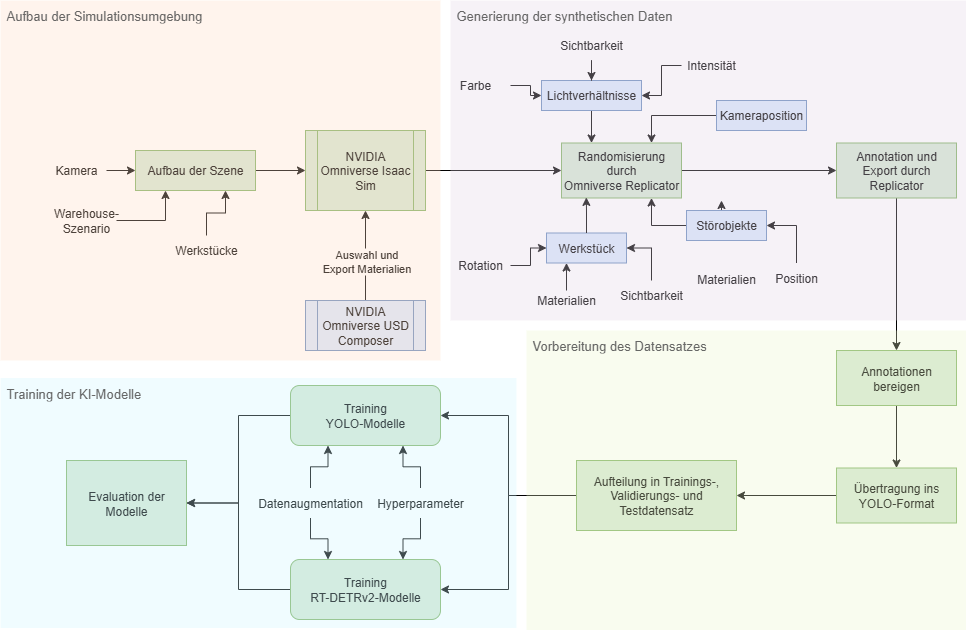
\includegraphics[width=0.9\linewidth]{graphics/Umsetzung_Diagramm.png}
    \caption{Grafische Visualisierung der Datengenerierungs- und Trainingspipeline}
    \label{fig:visualisierung_umsetzung}
\end{figure}

Abbildung \ref{fig:visualisierung_umsetzung} bietet eine grafische Übersicht über die in dieser Arbeit entwickelte Datengenerierungs- und Trainingspipeline.
Diese Pipeline wird im folgenden Kapitel detailliert beschrieben.

\section{Zielsetzung und Forschungsmethodik}
Ziel dieses Kapitels ist die praktische Umsetzung des in Kapitel \ref{sec:forschungsdesign} beschriebenen Forschungsdesigns. Der Fokus liegt auf der Realisierung einer Datenpipeline, mithilfe welcher automatisch synthetische Bilddaten inklusive deren Annotationen in einer Simulationsumgebung generiert werden. Die Pipeline soll so gestaltet sein, dass zentrale Parameter, die den Umfang und die Qualität der Daten betreffen, flexibel angepasst werden können. Darüber hinaus soll die Pipeline so konzipiert sein, dass sie leicht auf andere Fehlerfälle anpassbar ist, wodurch ihre Wiederverwendbarkeit und Übertragbarkeit auf andere Anwendungsszenarien sichergestellt wird. Die generierten Daten werden anschließend für das Training von \ac{KI}-Modellen aufbereitet. Darauf aufbauend erfolgt exemplarisch ein Training verschiedener Modelle und Modellarchitekturen zur Fehlererkennung, um die Qualität der durch die Pipeline erzeugten Daten zu validieren.

Methodisch folgt das Vorgehen dem \ac{DSR}-Paradigma, nach welchem das Artefakt in einem \textit{Build-and-Evaluate} Prozess entwickelt wird. Konkret wird das Artefakt in iterativen Zyklen entwickelt, getestet und verbessert. Dieses Kapitels konzentriert sich auf die Entwicklung des Artefakts, während eine detaillierte Evaluation der erzielten Ergebnisse in Kapitel \ref{chapter:Evaluation_Ergebnisse} folgt.


\section{Aufbau der Simulationsumgebung}

Im Sinne der Abbildung \ref{fig:visualisierung_umsetzung} wurden für die Umsetzung der Simulationsumgebung \textit{NVIDIA Omniverse}-Tools eingesetzt. Konkret kamen \textit{NVIDIA Omniverse USD Composer} auf Basis von \textit{Omniverse Kit} (Version 107.3.0) sowie \textit{NVIDIA Isaac Sim} (Version 4.5.0 rc.36) zum Einsatz. Diese Tools sind dafür bekannt, hochqualitative und realistische Bilddaten erzeugen zu können und wurden auch schon in ähnlichen Arbeiten, wie der Arbeit von \cite{monnet_investigating_2024} zur Generierung von Kratzern auf Metalloberflächen, verwendet.\footnote{Vgl. \cite[769 ff.]{monnet_investigating_2024}}

Der \textit{USD Composer} ist primär auf den Aufbau und die Gestaltung von \ac{CAD}-Szenen konzipiert\footcite{nvidia_omniverse_2025} und wurde in diesem Anwendungsfall hauptsächlich für die Auswahl und Speicherung unterschiedlicher Materialvarianten für das Werkstück und der Störobjekte verwendet. Der Großteil der Umsetzung erfolgte allerdings in \textit{Isaac Sim}\footcite{nvidia_isaac_2025}, da dort die Implementierung des \textit{Omniverse Replicator} eine effiziente Realisierung der \textit{Domain Randomization} sowie den Export der generierten Bilddaten ermöglichte.\footcite{nvidia_replicator_2025}

Als Grundlage der Simulationsumgebung diente ein von \textit{Isaac Sim} bereitgestelltes Warehouse-Szenario, welches aufgrund der bereits implementierten Beleuchtungselementen ausgewählt wurde. Hierdurch kann eine realitätsnahe Umsetzung, insbesondere in Hinblick auf die Lichtverhältnisse, erreicht werden. In die Szene wurde außerdem eine von TRUMPF bereitgestellte Fertigungsmaschine platziert sowie ergänzend 84 Zustände eines Blechs im Schneideprozess, einschließlich der vollständig ausgeschnittenen Teile. Die CAD-Dateien für Blech und Maschine wurden aus der Software \textit{Siemens NX} im USD-Format exportiert. Grundsätzlich können jedoch jegliche USD-Modelle eingebunden werden, wodurch die Simulationsumgebung flexibel erweiterbar bleibt. 

Zur Bildaufnahme wurde eine virtuelle Kamera implementiert, welche ebenfalls durch \textit{Isaac Sim} bereitgestellt wird. Diese wurde mit Parametern konfiguriert, die den realen Produktionskameras entsprechen, wodurch eine möglichst enge Annäherung an reale Produktionsszenarien erreicht werden kann.


\section{Generierung der synthetischen Bilddaten}

Aufbauend auf der in Abbildung \ref{fig:visualisierung_umsetzung} dargestellten Systematik erfolgte im Anschluss an den Aufbau der Simulationsumgebung die Generierung der Bilddaten mit zufälliger Variation zentraler Parameter im Sinne der \textit{Domain Randomization} mithilfe des \textit{Omniverse Replicator}.\footcite{nvidia_replicator_2025}
Bei dem \textit{Omniverse Replicator} handelt es sich um ein Framework, mithilfe welchem Pipelines zur Generierung umfassender synthetischer Daten gebaut werden können. Durch diesen ist es möglich, bestehende USD-Szenen zu Nutzen oder neue Szenen dynamisch aufzubauen. Verschiedene Elemente und deren Eigenschaften in der Szene können mit diesem Tool zufällig variiert, automatisch annotiert und exportiert werden.\footnote{Vgl. \cite{nvidia_replicator_2025}}

Aufgrund zeitlicher Beschränkungen wurde exemplarisch ein konkreter Anwendungsfall umgesetzt, der wie folgt definiert ist:
Ein vollständig ausgeschnittenes Blech wird auf der Maschine platziert und die ausgeschnittenen Teile für jedes Bild zufällig in die vorgesehen Aussparung zurück platziert. Die Teile werden dabei zufällig um einen Winkel rotiert, deren Spannweite durch einen Parameter in der Pipeline festgelegt werden kann. In diesem Anwendungsfall betrug der Rotationsbereich -4° bis +4° relativ zur Ausgangsposition. Weitere potenzielle Szenarien, wie beispielsweise verschobene oder nicht vollständig herausgetrennte Teile, konnten aufgrund zeitlicher Einschränkungen nicht mehr implementiert werden, können jedoch aufgrund der flexiblen Architektur problemlos ergänzt werden.

Neben der Variation der Werkstücke wurden auch Umgebungsparameter randomisiert. Dazu zählen insbesondere die Materialien des Blechs und der ausgeschnittenen Teile sowie die Umgebungsbeleuchtung. Bei letzterer wurde sowohl die Sichtbarkeit einzelner Lichter als auch deren Intensität und Farbe zufällig variiert. Zudem wurde die Position der Kamera randomisiert, wobei sowohl die Entfernung zum Werkstück, als auch die horizontale und vertikale Position innerhalb vorgegebener Grenzen variiert wurde. Auf diese Weise sollte die Robustheit des Modells gegenüber unterschiedlicher Blickwinkel und Bildausschnitte erhöht werden.

Zentrale Parameter der Pipeline können zu Beginn des Skripts nach Bedarf angepasst werden. Hierzu zählen verschiedene  Einstellungen zur Bildqualität, wie beispielsweise Antialiasing, Bildauflösung und Parameter zur Simulation des Lichts. Auch die Konfiguration der \textit{Domain Randomization} kann im Skript angepasst werden. Die konkrete Implementierung der Datengenerierungspipeline ist in Anhang \ref{anhang:replicator_code} aufgeführt.\footnote{Vgl. Anhang \ref{anhang:replicator_code}}

\begin{figure}[htb]
    \centering
    \begin{subfigure}{0.49\textwidth}
        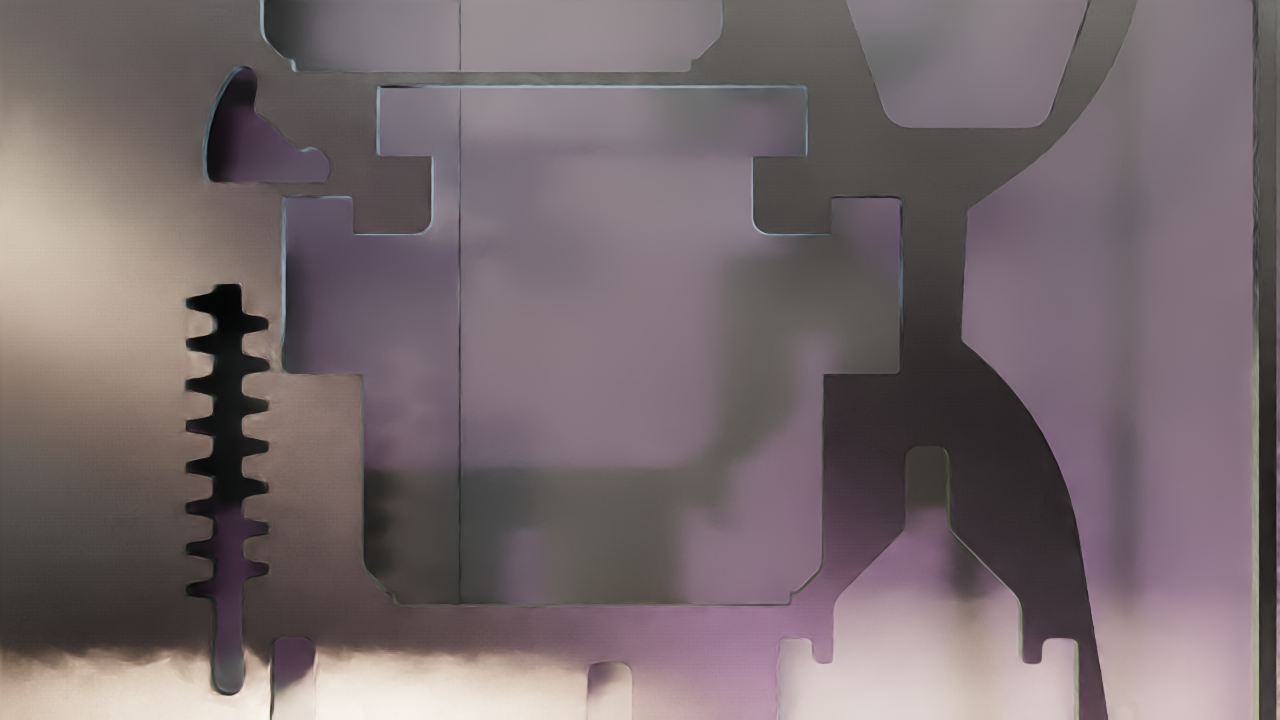
\includegraphics[width=\textwidth]{graphics/example_synthetic_images/Beispiel_Replicator_1.png}
    \end{subfigure}
    \hfill
    \begin{subfigure}{0.49\textwidth}
        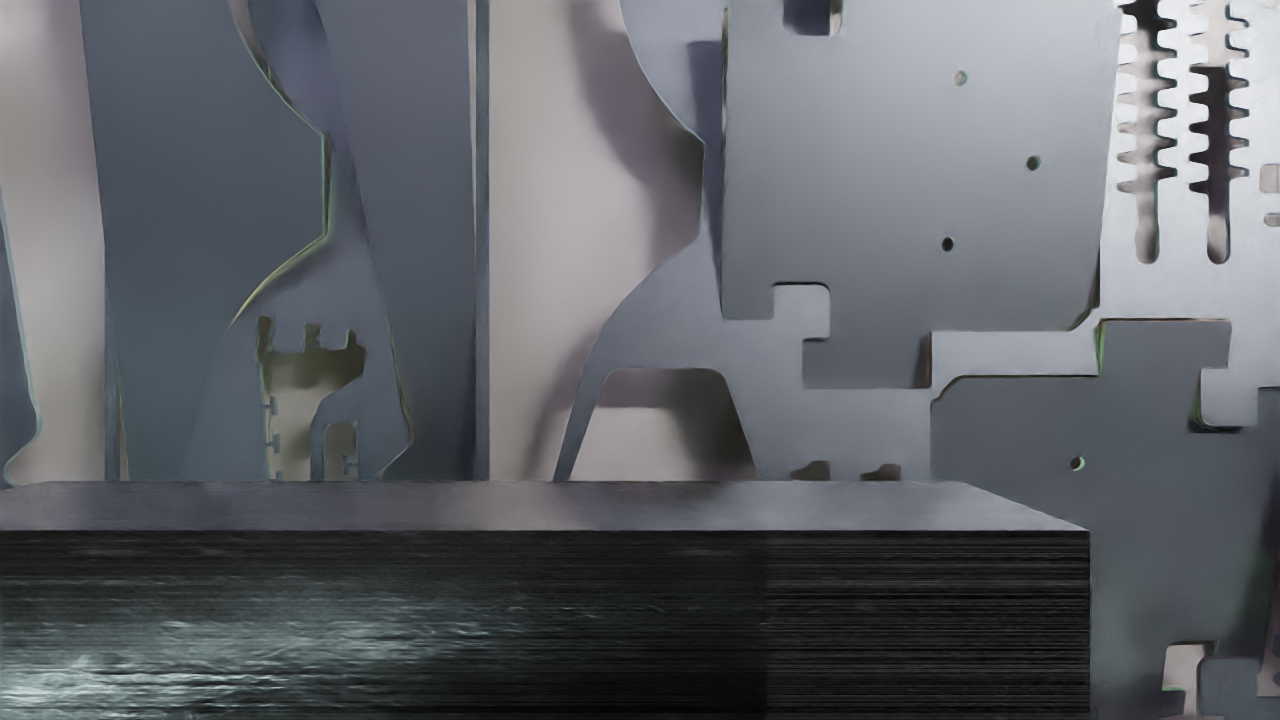
\includegraphics[width=\textwidth]{graphics/example_synthetic_images/Beispiel_Replicator_2.png}
    \end{subfigure}
    \caption{Beispiele für exportierte Bilder aus dem Replicator}
    \label{fig:beispiel_replicator}
\end{figure}

Abbildung \ref{fig:beispiel_replicator} zeigt zwei beispielhafte Bilder, welche mithilfe des Replicators generiert wurden. Insgesamt wurden 1077 Bilder exportiert. Ein größerer Umfang wäre prinzipiell möglich gewesen, war jedoch aufgrund der verfügbaren Rechenleistung und des damit verbundenen Zeitaufwands im Rahmen dieser Arbeit nicht umsetzbar. 

Diese Bilddaten werden dabei durch den Replicator automatisch annotiert. Ein Beispiel hierfür ist in Abbildung \ref{fig:replicator_annotationen} dargestellt. Zwar liegen die exportierten Annotationen im Textformat vor, für dieses Beispiel wurden sie jedoch zur Veranschaulichung visualisiert.

\begin{figure}[htb]
    \centering
    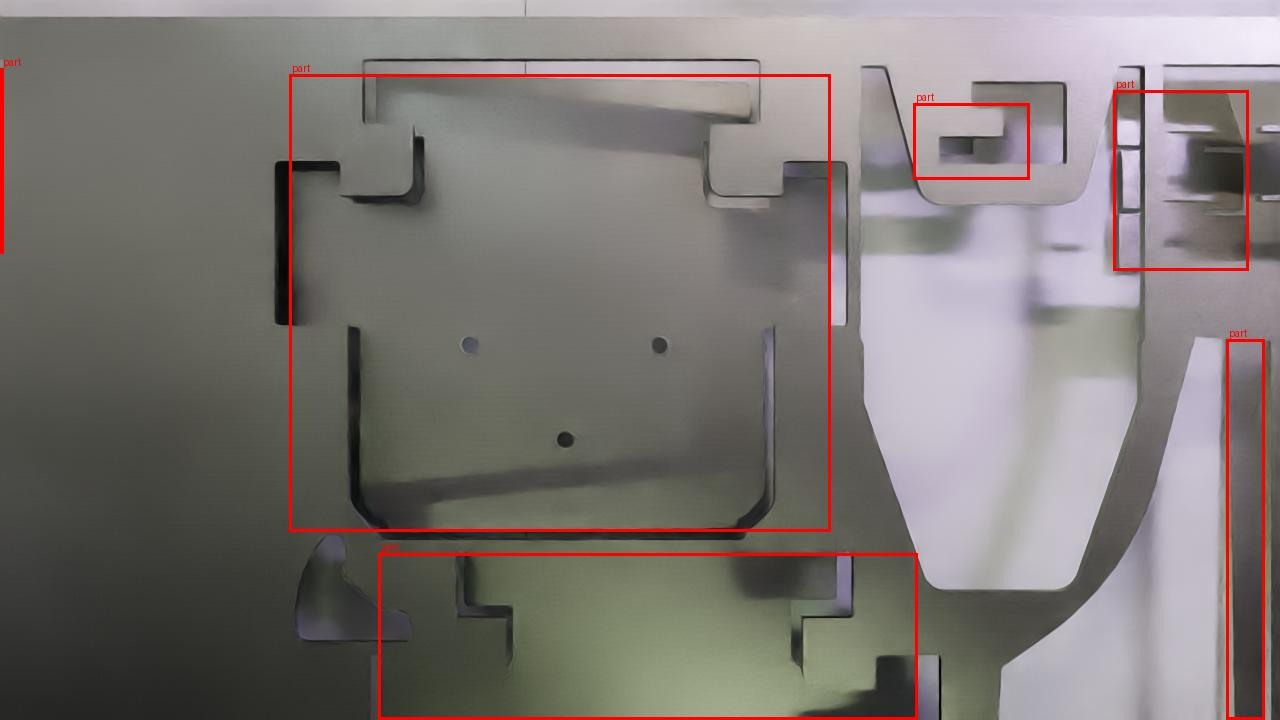
\includegraphics[width=0.9\linewidth]{graphics/example_synthetic_images/Beispiel_Annotation.jpg}
    \caption{Beispiel einer durch den Replicator automatisch erzeugten Annotation (grafisch visualisiert)}
    \label{fig:replicator_annotationen}
\end{figure}


\section[Training von KI-Modellen auf synthetischen Bilddaten]{Training von \ac{KI}-Modellen auf synthetischen Bilddaten}

\subsection{Auswahl der KI Architekturen und Modelle}
Als erstes Modell wurde die \ac{YOLO}-Architektur ausgewählt, welche auf \acp{CNN} basiert und sich in zahlreichen Benchmarks als leistungsfähiger und effizienter Standard im Bereich der Objekterkennung erwiesen hat. \footnote{Vgl. \cite[771]{monnet_investigating_2024}; \cite{bilous_comparison_2024}}
Verwendet wurde dabei die Implementierung von \textit{Ultralytics}, die aufgrund ihrer einfachen Handhabung, umfangreicher Dokumentation und integrierter Möglichkeiten zur Datenaugmentation ein besonders praxistaugliches Framework bietet.\footnote{Vgl. \cite{yolo11_ultralytics}}
Aufgrund begrenzter Hardwarekapazitäten konzentrierte sich diese Arbeit auf das Training kleinerer Modellvarianten (Nano, Small und Medium).

Angesichts der kleinen Größe des Datensatzes und der Handhabung von synthetischen Daten wurde ein relativ hoher Grad an Datenaugmentation beim Training eingesetzt, um die Generalisierungsfähigkeit der Modelle zu verbessern.

\subsection{Vorbereitung des Datensatzes und Training der Modelle}
Vor dem tatsächlichen Training der \ac{KI}-Modelle wurden die durch den \textit{Omniverse Replicator} exportierten Bild- und Annotationsdaten im Sinne der Abbildung \ref{fig:visualisierung_umsetzung} zuerst in ein geeignetes Format überführt. Der Export aus dem Replicator erfolgte im sogenannten KITTI-Format, welches sich nicht unmittelbar für die nachfolgenden Trainingspipelines eignete. Für das Training der \ac{YOLO}-Modelle mussten die Annotationsdaten in das \ac{YOLO}-Format konvertiert werden. Dazu wurden Bild- und Annotationsdateien in einer automatisierten Pipeline konsolidiert, das Format der Annotationsdaten angepasst und der Datensatz in Trainings-, Validierungs- und Test-Splits unterteilt.\footnote{Vgl. Anhang  \ref{anhang:datensatz_erstellen_code}} Dabei wurde ein Split von 70/20/10 (70\% Training, 20\% Validierung, 10\% Test) gewählt, was eine anerkannte Aufteilung in der Literatur darstellt.\footnote{Vgl. 
\cite[261]{urgo_monitoring_2024}; \cite[3]{griem_synthetic_2025}; \cite[5]{khirodkar_domain_2018}}

Auf diesem Datensatz wurden drei Modelle der YOLO11-Architektur trainiert (Nano, Small und Medium). Um die effektive Größe und Varianz des Trainingsdatensatzes zu erhöhen, kamen umfangreiche Verfahren der Datenaugmentation zum Einsatz, welche durch das Trainingsframework von \textit{Ultralytics} bereitgestellt werden.\footnote{Vgl. Anhang \ref{anhang:yolo_code}} Die Auswahl der Hyperparameter bestimmte sich primär aus der offiziellen Dokumentation von \textit{Ultralytics}\footnote{Vgl. \cite{ultralytics_hyperparameter-optimierung_nodate}; \cite{ultralytics_yolo-datenerweiterung_nodate}} sowie einem iterativen Trainingsansatz.\footnote{ChatGPT-5 wurde unterstützend bei der Optimierung der Hyperparameter eingesetzt.} Die Anzahl der Epochen wurde auf 200 festgelegt, mit dem Ziel, durch eine hohe Augmentierung in Kombination mit einer hohen Anzahl an Epochen den kleinen Datensatz bestmöglich auszunutzen und \textit{Overfitting} zu vermeiden.

Neben den \ac{YOLO}-Modellen wurde ergänzend ein transformerbasiertes Modell trainiert. Da herkömmliche Transformer-Architekturen bei kleinen Datensätzen ineffizient sind, wurde der \ac{RT-DETR}v2 gewählt, eine speziell optimierte Variante für ressourcenschonendes Training \footnote{Vgl. \cite{zhao_detrs_2023}}.
Hier wurde sowohl ein Modell mit Datenaugmentation als auch eines ohne Datenaugmentation trainiert. Aus zeitlichen Gründen wurde hierbei ausschließlich eine kleinere Variante (\ac{RT-DETR}-18) eingesetzt.\footnote{Vgl. Anhang \ref{anhang:rt_detr_code}} Auch hier wurde eine hohe Anzahl an Epochen (220) gewählt, um den kleinen Datensatz bestmöglich auszuschöpfen. Allerdings konvergierten beide Modelle bereits nach kurzer Zeit und beendeten das Training bereits nach etwa 40 Epochen, da keine weiteren Verbesserungen erzielt werden konnten.

\subsection{Probleme während des Trainings}
Im Rahmen der Evaluation traten spezifische Probleme im Datenpipeline-Design auf. So zeigte sich, dass die mit dem KITTI-Writer erzeugten Bounding Boxes fehlerhaft erzeugt wurden, wodurch mehr Annotationen als tatsächlich Objekte vorhanden waren. Dies hatte zur Folge, dass Bounding Boxes nicht mit den tatsächlichen Objektpositionen übereinstimmten, was eine Bereinigung der Annotationsdaten erforderlich machte. Zudem wurden teilweise Bild-Label-Paare doppelt in verschiedenen Datensplits abgelegt (\textit{Data Leakage}), was zu einer Überschätzung der Modellleistung in der Validierung führte. Diese Inkonsistenzen wurden behoben und die Trainingsläufe wiederholt.


\subsection[Evaluation der KI-Modelle]{Evaluation der \ac{KI}-Modelle}\label{subsec:umsetzung_evaluation_modelle}
Die trainierten Modelle wurden zunächst auf dem zuvor definierten Test-Split des synthetischen Datensatzes evaluiert.\footnote{Vgl. Anhang \ref{anhang:evaluation_yolo_code} und Anhang \ref{anhang:evaluation_rtdetr_code}} Anhand der in Abschnitt \ref{subsec:evaluationsdesign} beschriebenen Metriken konnte so eine erste Einschätzung der Modellleistung erfolgen. Bei unzureichenden Ergebnissen wurden Trainingsparameter angepasst und das Training erneut durchgeführt. Durch diesen iterativen Prozess konnte die Modellleistung auf synthetischen Daten stetig verbessert werden.

Wie bereits in Abschnitt \ref{subsec:evaluationsdesign} beschrieben, wurden die Modellvorhersagen vor der Berechnung der Metriken einem \ac{NMS} unterzogen. Hierbei wurde eine \ac{IoU}-Schwelle von 0.5 verwendet, welches ein üblicher Wert in der Praxis darstellt.\footnote{Vgl. \cite[8]{he_mask_2017}; \cite[3]{bodla_soft-nms_2017}} Überlappende Bounding Boxes mit einem Überschneidungsgrad von 50\% werden dementsprechend durch \ac{NMS} reduziert.

Um die Generalisierungsfähigkeit der Modelle und ihre Übertragbarkeit auf reale Anwendungsfaälle zu überprüfen, wurde die Modellleistung ergänzend auf realen Bildern evaluiert.\footnote{Vgl. Anhang \ref{anhang:evaluation_yolo_code} und Anhang \ref{anhang:evaluation_rtdetr_code}} Dazu wurde aus \textit{TRUMPF Visual Insights}, einer unternehmensinternen Software, in welcher Videos der Produktionsmaschinen bei Fehlerfällen gespeichert sind, 34 Bilder gesammelt, welche dem simulierten Fehlerfall ähnelten. Diese Bilder wurden manuell annotiert und dienten als unabhängiger Referenzdatensatz zur abschließenden Evaluation der Modelle. Bei unzureichender Leistung wurde auch hier das Training mit angepassten Parametern wiederholt, wobei die Anzahl an Iterationen aufgrund zeitlicher Limitationen eingeschränkt war.




\chapter[Evaluation der KI-Modelle zur Fehlererkennung bei Werkzeugmaschinen]{Evaluation der \ac{KI}-Modelle zur Fehlererkennung bei Werkzeugmaschinen \footnote{Sprachlich geglättet durch ChatGPT-5}}
\label{chapter:Evaluation_Ergebnisse}

\section{Zielsetzung und Forschungsmethodik}
Ziel der Evaluation ist, die Leistungsfähigkeit der auf synthetischen Daten trainierten \ac{KI}-Modelle zur Erkennung von Fehlerfällen bei Werkzeugmaschinen zu überprüfen. Dabei wird sowohl die Leistung der KI-Modelle auf synthetischen Daten als auch der Übertrag auf die Realität durch Tests auf realen Daten betrachtet. Dies schafft eine Basis, auf welcher die Eignung synthetischer Daten für Anwendungszwecke solcher Art diskutiert werden kann.

Methodisch orientiert sich die Evaluation am im Kapitel \ref{subsec:evaluationsdesign} dargestellten Design. Zunächst werden die Modelle auf dem Test-Split des synthetischen Datensatzes evaluiert, um einen ersten Eindruck der Leistungs- und Generalisierungsfähigkeit zu erlangen. Gleichzeitig dient dieser Schritt der Validierung der Pipeline zur Datengenerierung, da hierdurch Konsistenz und Eignung synthetischer Bilddaten für das Training von \ac{KI}-Modellen untersucht werden kann.

Ergänzend erfolgt eine Evaluation auf einem realen Testdatensatz aus 34 Bildern, welcher wie in Kapitel \ref{subsec:umsetzung_evaluation_modelle} beschrieben zusammengestellt und annotiert wurde. Diese Untersuchung dient primär der Analyse der Eignung von auf synthetischen Daten trainierten Modellen in realen Anwendungsumgebungen sowie der Betrachtung des Einflusses des \textit{Domain Gaps}. Auf dieser Grundlage lässt sich auch der Bedarf an zukünftiger Forschung in diesem Themengebiet ableiten.


\subsection[Evaluation der YOLO-Modelle]{Evaluation der \ac{YOLO}-Modelle}

Zuerst wurden die drei \ac{YOLO}-Modelle auf dem synthetischen Datensatz evaluiert. Der Verlauf zentraler Metriken während des Trainings ist exemplarisch für das \ac{YOLO}-Medium Modell in Abbildung \ref{fig:training_verlauf} dargestellt. Es ist zu erkennen, dass die Modelle bereits nach wenigen Epochen eine gute Leistung auf dem Validierungsdatensatz erzielen konnten und schlussendlich eine Konvergenz zu erkennen ist. Ein ähnlicher Verlauf zeigte sich auch bei den beiden anderen Modellvarianten.\footnote{Vgl. Anhang \ref{anhang:training_verlauf}}

\begin{figure}[htb]
      \centering                        
      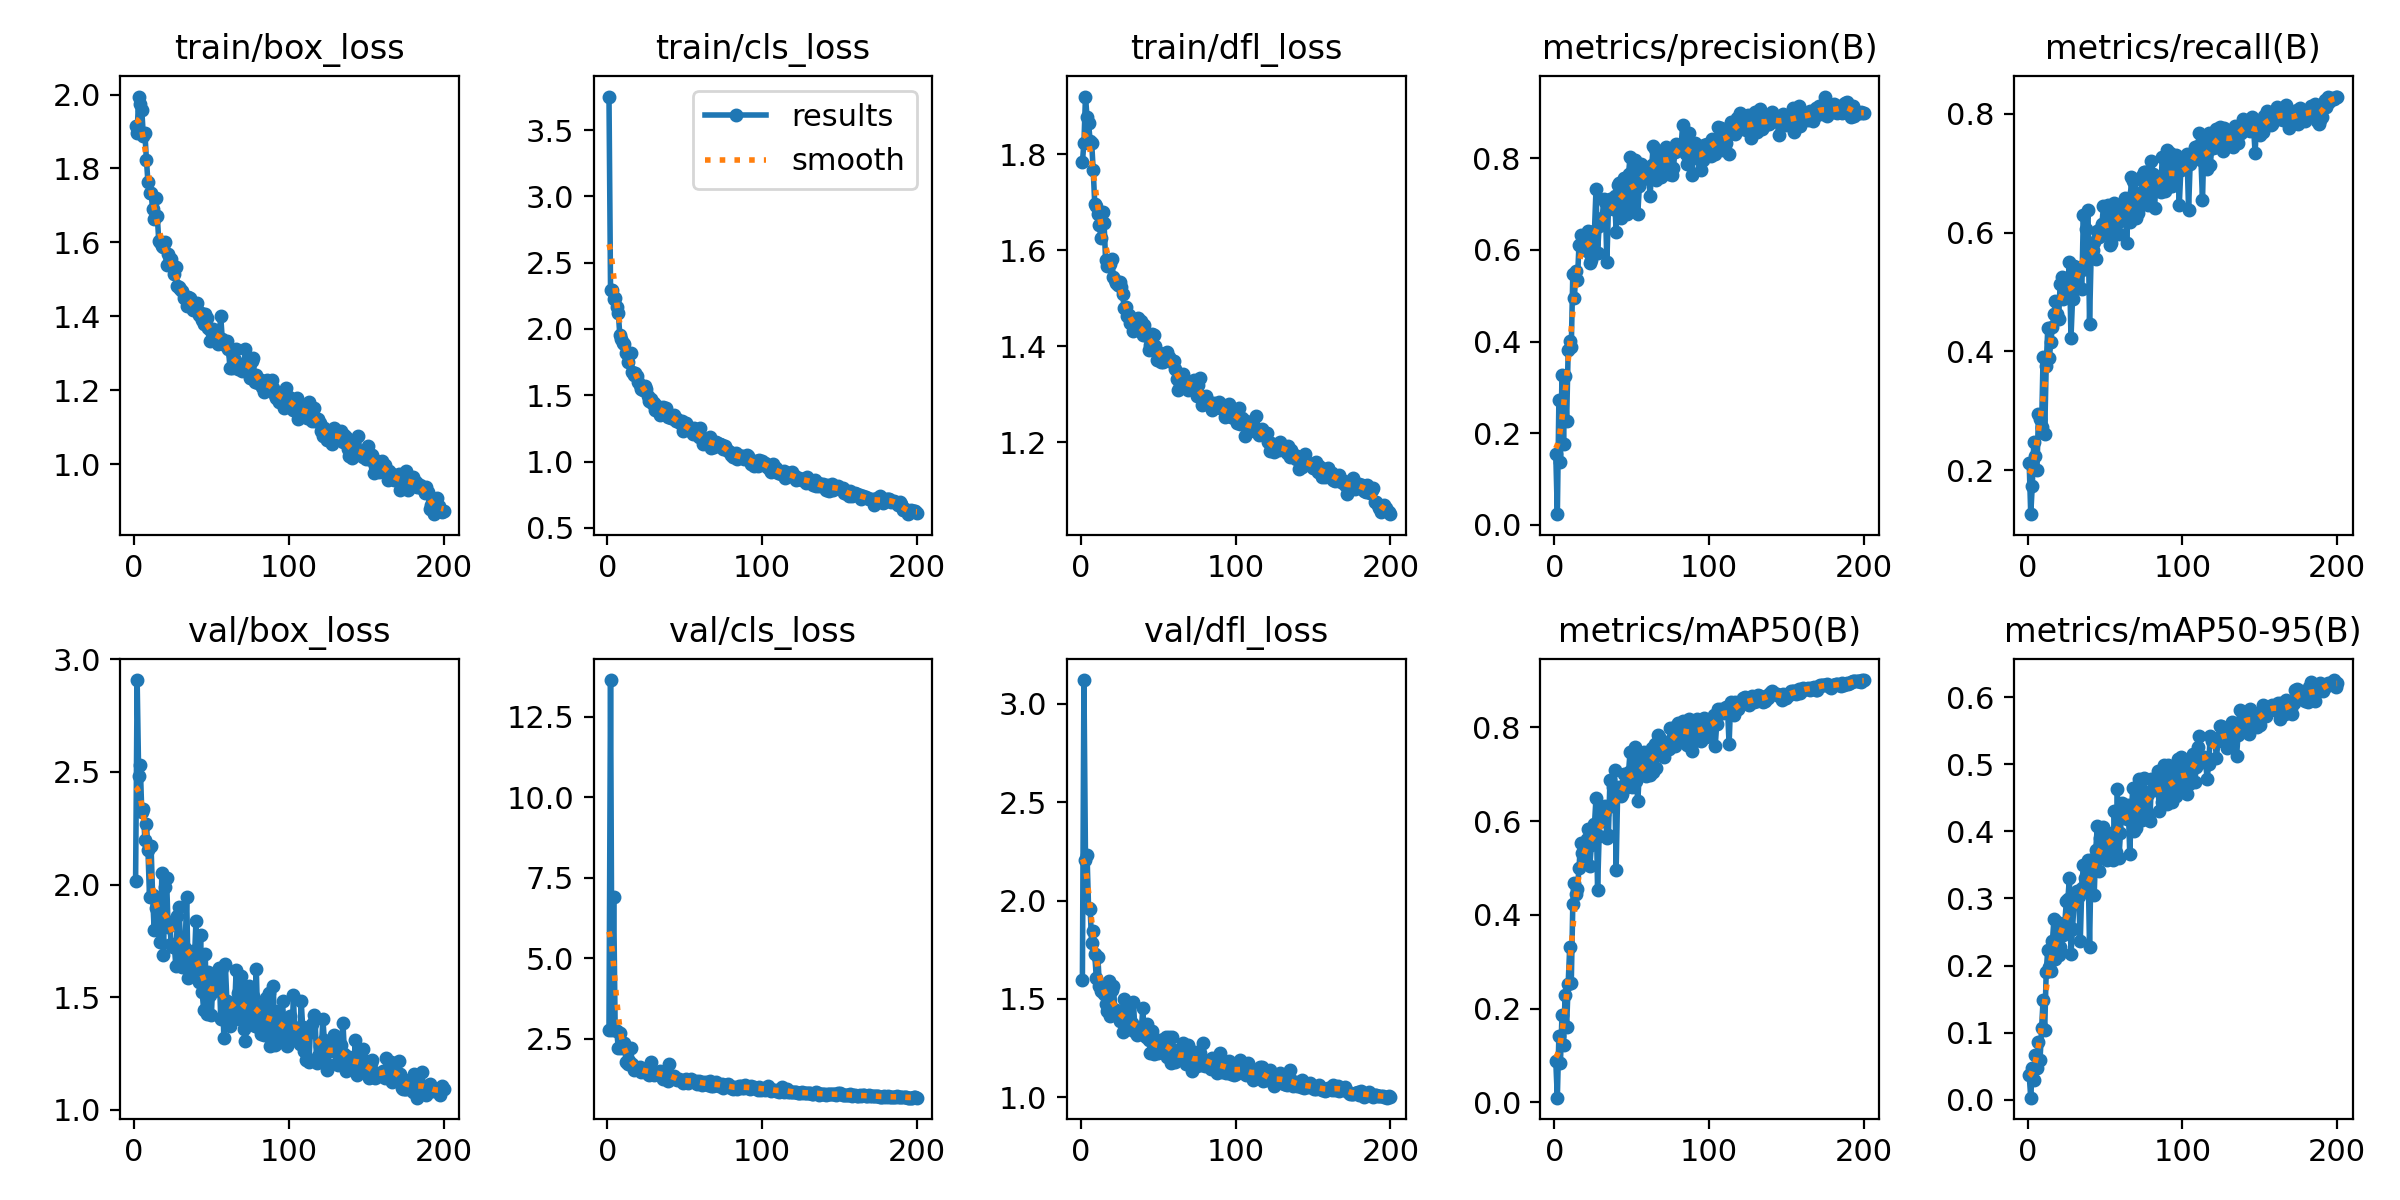
\includegraphics[width=0.9\linewidth]{graphics/yolo_eval/model_m/results.png}
      \caption{Trainingsverlauf des \ac{YOLO}-Modells Medium}
      \label{fig:training_verlauf}
\end{figure}

Wie in Tabelle \ref{tab:yolo_results} dargestellt, zeigten alle drei Modelle eine konsistente Leistung auf dem synthetischen Test-Split. Das \ac{YOLO}-Small Modell erzielte dabei die beste Leistung mit einer \ac{mAP}@50 von 0.9080 und einer \ac{mAP}@[.5:.95] von 0.6605. Auch beim Sensitivität Wert erreichte dieses Modell mit 0.8094 den höchsten Wert. Bei allen drei Modellen lag die Präzision über 0.9, was auf eine geringe Rate an \ac{FP} hinweist.  Es ist jedoch zu beachten, dass alle Modelle bei allen Metriken nahe beieinander liegen und keine signifikanten Unterschiede zwischen dem kleinsten und dem größten Modell erkennbar waren. 

Abbildung \ref{fig:pr_kurven} zeigt ergänzend die Präzisions-Sensitivitäts-Kurven des größten und kleinsten trainierten Modells. Beide Kurven zeigen einen ähnlichen Verlauf, wobei das \ac{YOLO}-Medium Modell etwas höhere Präzisions-Werte bei höherer Sensitivät erreichte. Insgesamt zeigen alle Modelle jedoch keine signifikanten Unterschiede,\footnote{Vgl. Anhang \ref{anhang:pr_curve_small}}sondern vergleichbar gute Ergebnisse auch bei hohen Sensitivitätswerten. 
Zusammenfassend lässt sich festhalten, dass alle drei Modelle auf dem synthetischen Datensatz eine gute Leistung erbringen konnten, was die Konsistenz und Eignung der mittels der Pipeline generierten synthetischen Daten für das Training von \ac{KI}-Modellen unterstreicht.

\begin{figure}[htb]
    \centering
    \begin{subfigure}{0.49\textwidth}
        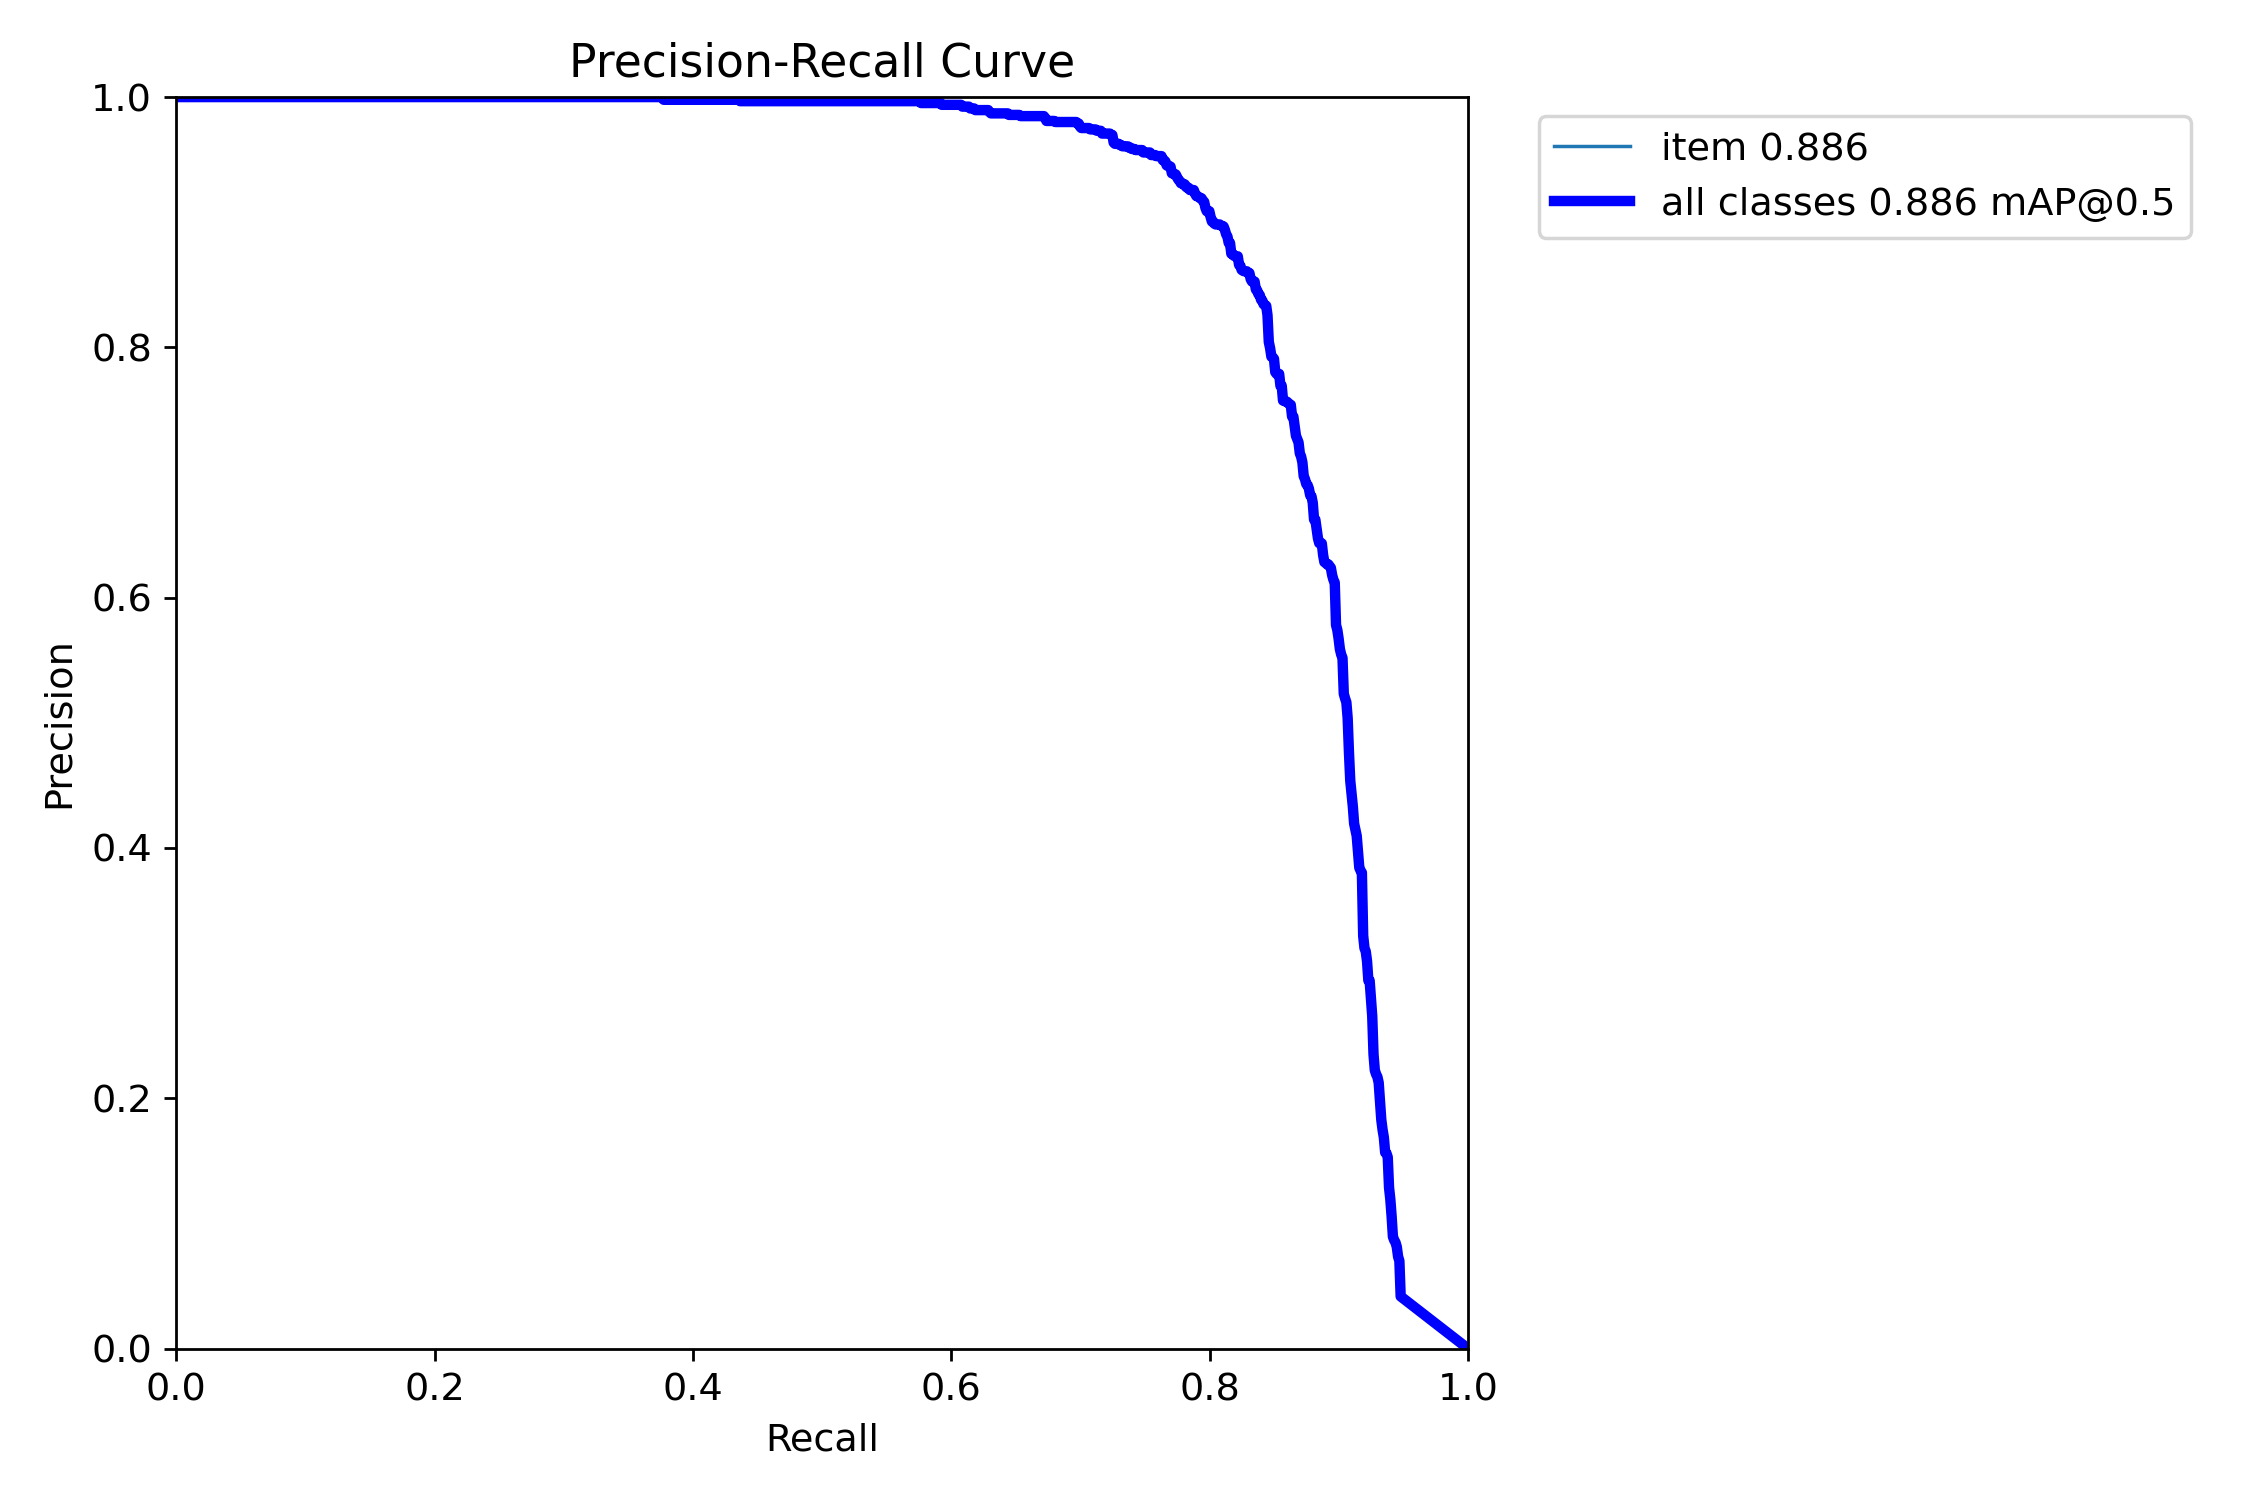
\includegraphics[width=\textwidth]{graphics/yolo_eval/model_n/BoxPR_curve.png}
        \caption{\ac{YOLO}-Modell Nano}
    \end{subfigure}
    \hfill
    \begin{subfigure}{0.49\textwidth}
        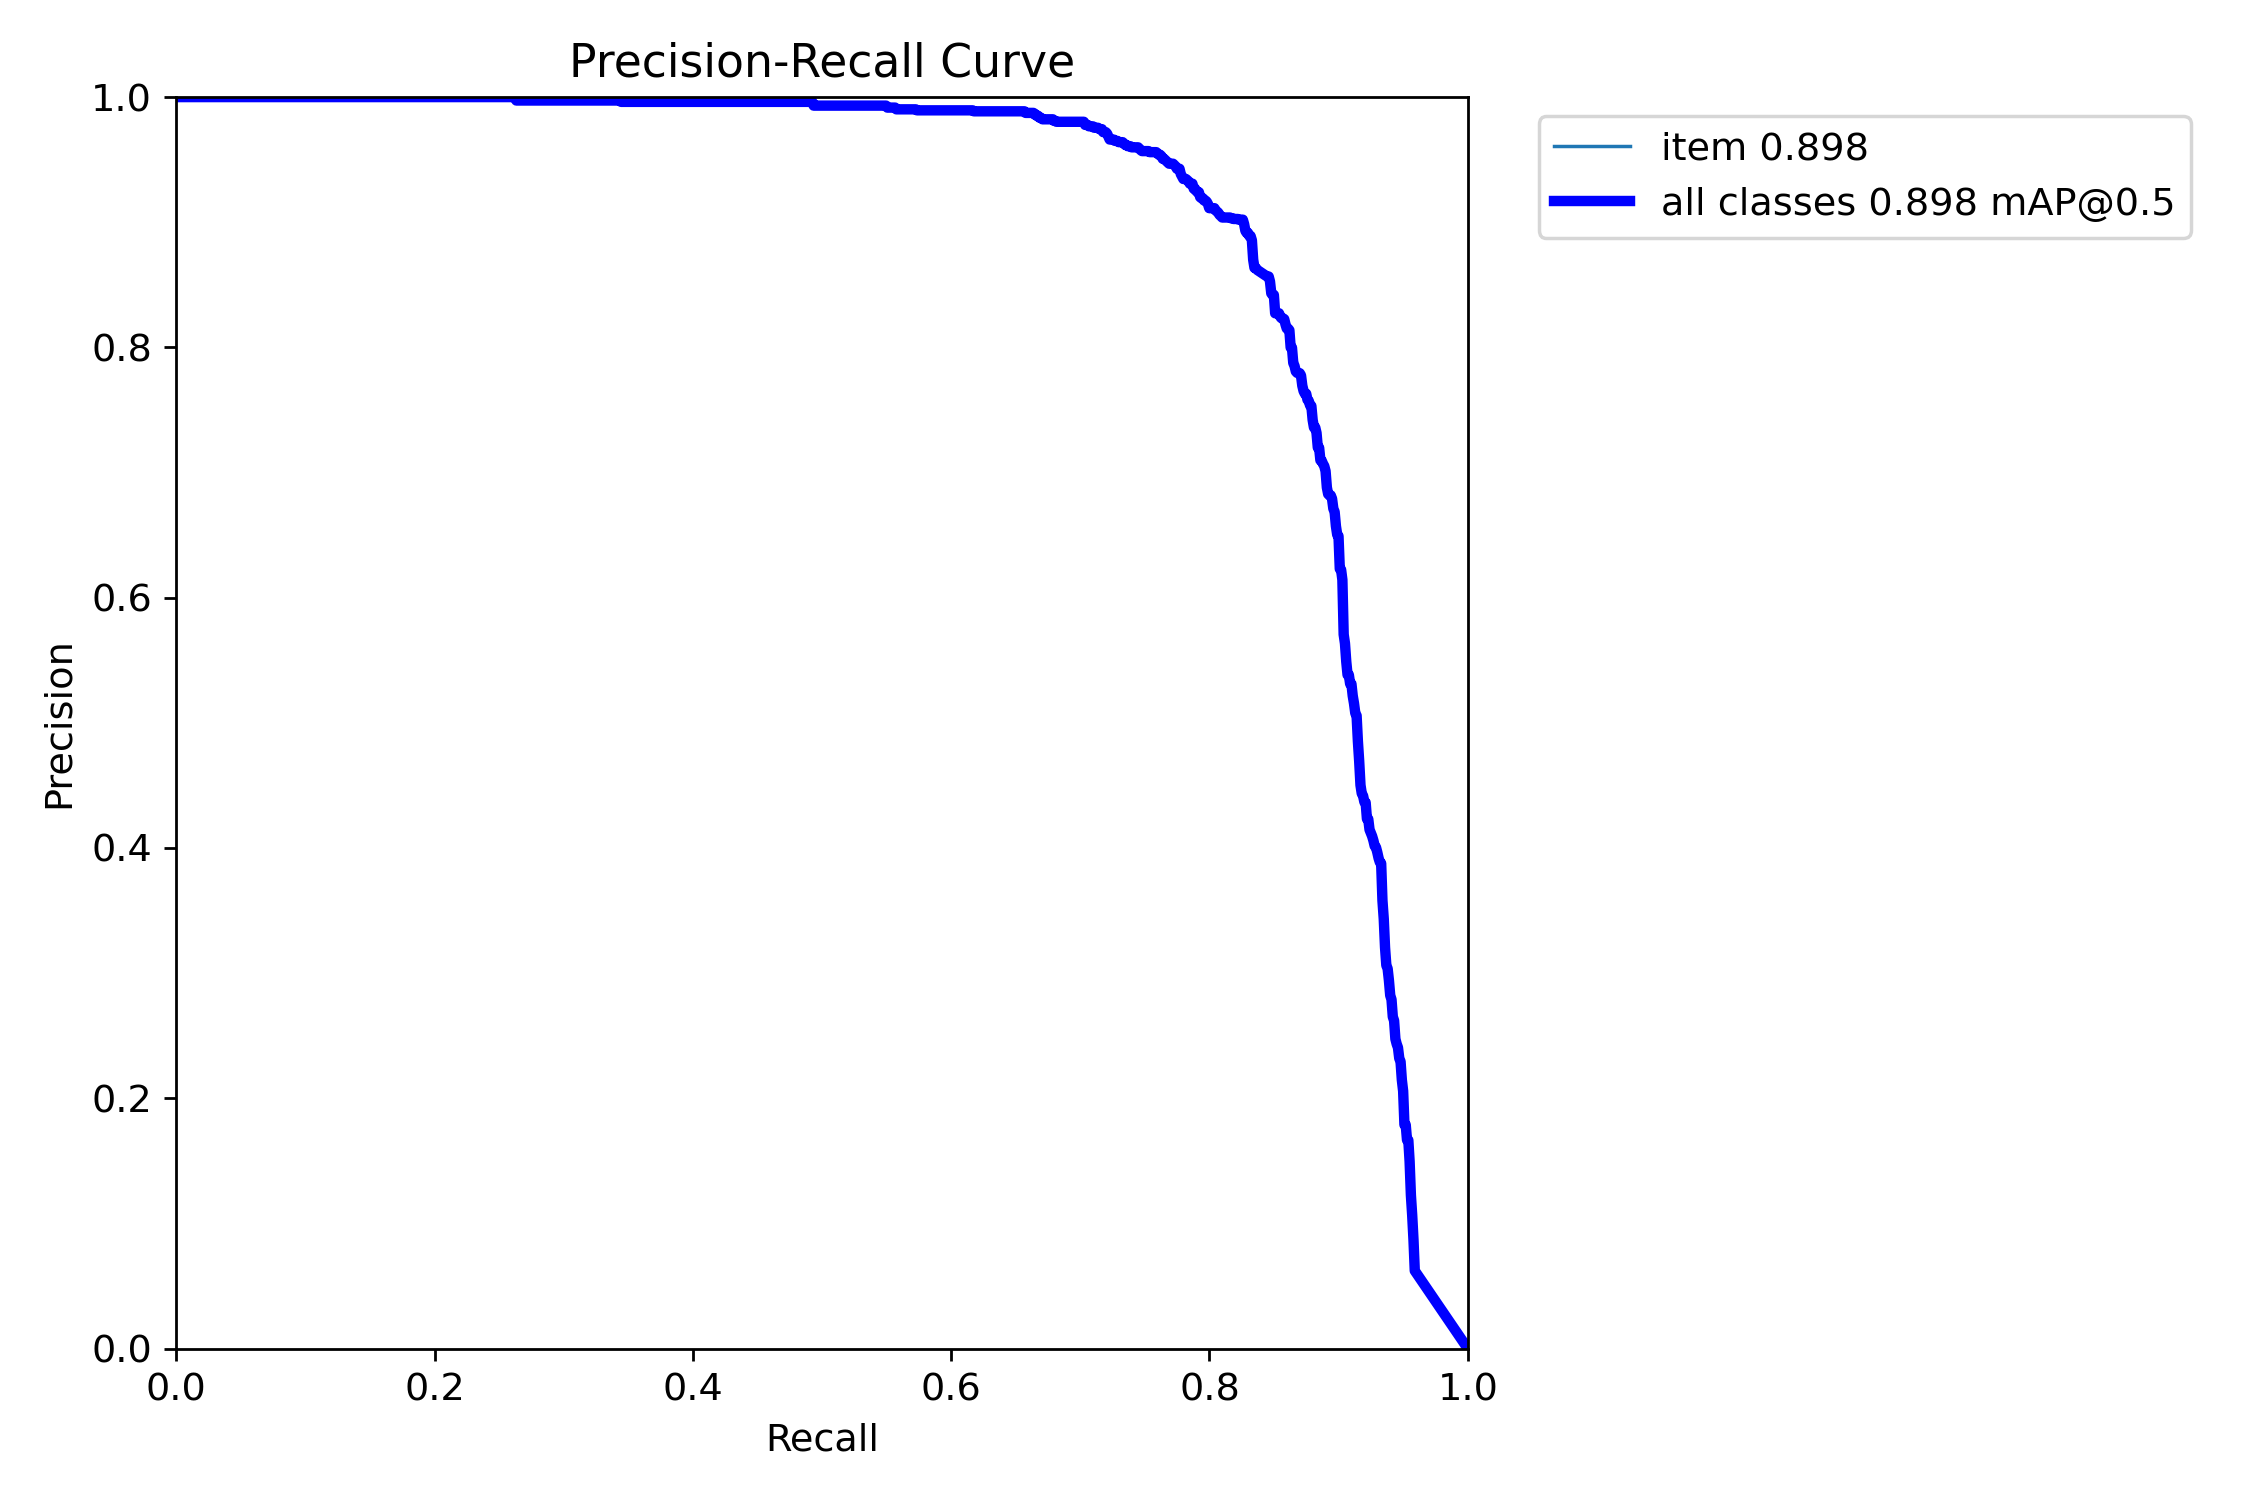
\includegraphics[width=\textwidth]{graphics/yolo_eval/model_m/BoxPR_curve.png}
        \caption{\ac{YOLO}-Modell Medium}
    \end{subfigure}
    \caption{Präzision-Sensitivität-Kurven der \ac{YOLO}-Modelle Nano und Medium}
    \label{fig:pr_kurven}
\end{figure}


Auf dem realen Datensatz hingegen zeigten alle drei \ac{YOLO}-Modelle eine deutlich reduzierte Leistung. Das \ac{YOLO}-Medium-Modell erzielte mit einer \ac{mAP}@50 von 0.0712 die beste Leistung, kann jedoch mit der erbrachten Leistung nicht als zufriedenstellend angesehen werden. Die anderen beiden Modelle wiesen einen noch stärkeren Leistungsabfall auf. Alle Modelle hatten hier deutlich geringe Präzisions- und Sensitivität-Werte, was auf eine höhere Anzahl an \ac{FP} und \ac{FN} schließen lässt. Dies verdeutlicht den Einfluss des \textit{Domain Gaps}, da die Modelle, obwohl sie auf synthetischen Daten gute Ergebnisse lieferten, Schwierigkeiten hatten, ihre Leistung auf reale Anwendungsfälle zu übertragen und zeigten aufgrund der geringen Anzahl an \ac{TP} keine Konsistenz in der korrekten Erkennung von Fehlerfällen.

\begin{table}[htb]
\centering
    \resizebox{\textwidth}{!}{
    \begin{tabular}{||c c c c c c c||} 
        \hline
        Modell & Datensatz & Augmentierung & \ac{mAP}@50 & \ac{mAP}@[.5:.95] & Präzision & Sensitivität \\ [0.5ex] 
        \hline\hline
        YOLO-n & synthetisch & ja & 0.8872 & 0.6628 & 0.9368 & 0.7510 \\ 
        \hline
        YOLO-s & synthetisch & ja & 0.9176 & 0.6673 & 0.9156 & 0.8250 \\
        \hline
        YOLO-m & synthetisch & ja & 0.8957 & 0.6607 & 0.9153 & 0.7996 \\ 
        \hline
        RT-DETR-v2-r18 & synthetisch & ja & 0.2790 & 0.1892 & 0.1966 & 0.6335 \\ 
        \hline
        RT-DETR-v2-r18 & synthetisch & nein & 0.5160 & 0.3913 & 0.1634 & 0.8070 \\ 
        
        \hline\hline
        
        YOLO-n & real & ja & 0.0161 & 0.0062 & 0.0425 & 0.0667 \\ 
        \hline
        YOLO-s & real & ja & 0.0115 & 0.0028 & 0.0240 & 0.1000 \\
        \hline
        YOLO-m & real & ja & 0.0712 & 0.0402 & 0.1087 & 0.1000 \\
        \hline
        RT-DETR-v2-r18 & real & ja & 0.0050 & 0.0020 & 0.0066 & 0.4000 \\ 
        \hline
        RT-DETR-v2-r18 & real & nein & 0.0052 & 0.0016 & 0.0066 & 0.4667 \\ 
        \hline
    \end{tabular}
    }
\caption{Ergebnisse zentraler Metriken der \ac{KI}-Modelle mit \textit{Confidence Threshold 0.1}}
\label{tab:yolo_results}
\end{table}


\subsection[Evaluation des RT-DETR Modells]{Evaluation des \ac{RT-DETR} Modells}

Betrachtet man die Ergebnisse der beiden \ac{RT-DETR}-r18-Modelle, so zeigt sich ein deutlich anderes Bild als bei den \ac{YOLO}-Modellen. Trotz der schnellen Konvergenz erzielten beide Modelle bereits auf dem synthetischen Test-Split eine signifkant schlechtere Leistung als alle drei \ac{CNN}-basierten Modelle. Auffällig ist dabei, dass die bessere Leistung das Modell, welches ohne Datenaugmentierung trainiert wurde, erzielen konnte. Dieses erreichte jedoch dennoch nur eine \ac{mAP}@50 von 0.5160 und eine \ac{mAP}@[.5:.95] von 0.3913. Besonders auffällig sind die sehr niedrigen Präzisions-Werte bei beiden Trainingsansätzen, was auf eine hohe Rate an \ac{FP} hinweist, während beim Sensitivität mit 0.8070 beim Training ohne Datenaugmentation ein vergleichsweiser akzeptabler Wert erreicht werden konnten. Dies deutet darauf hin, dass das Modell zwar einige der tatsächlichen Fehlerfälle erkennt, jedoch auch viele \ac{FP} generiert. Angesichts dieser hohen Zahl an \ac{FP} ist keine Konsistenz in der korrekten Erkennung ersichtlich und es könnte sich auch um zufällige Treffer handeln.

Bei der Evaluation auf dem realen Datensatz verschlechterte sich die Leistung beider Modelle weiter. Mit \ac{mAP}@50 und \ac{mAP}@[.5:.95] Werten nahe 0 zeigten die Modelle eine nahezu unbrauchbare Leistung. Sowohl Präzisions als auch Sensitivitäts-Werte fielen im Vergleich zu dem synthetischen Datensatz nochmals deutlich ab. Daraus ist abzuleiten, dass die Modelle zwar viele Elemente des Bildes als Fehler klassifizieren, jedoch kaum korrekte Vorhersagen treffen und tatsächliche Fehler übersehen. Betrachtet man die in Abbildung \ref{fig:beispiel_vorhersage_rtdetr} dargestellte visualisierte Vorhersage des Modells mit Datenaugmentierung, wird dieser Verdacht bestätigt. Es sind zahlreiche \textit{Bounding Boxes} zu erkennen, welche jedoch kaum mit den tatsächlichen Fehlern übereinstimmen. Damit kann zusammengefasst werden, dass die \ac{RT-DETR}-Modelle sowohl auf synthetischen als auch auf realen Daten eine deutlich schlechtere Leistung erbrachten als die \ac{YOLO}-Modelle und auf keinem der Datensätze eine zufriedenstellende Leistung aufweisen konnten.

\begin{figure}[htb]
      \centering                        
      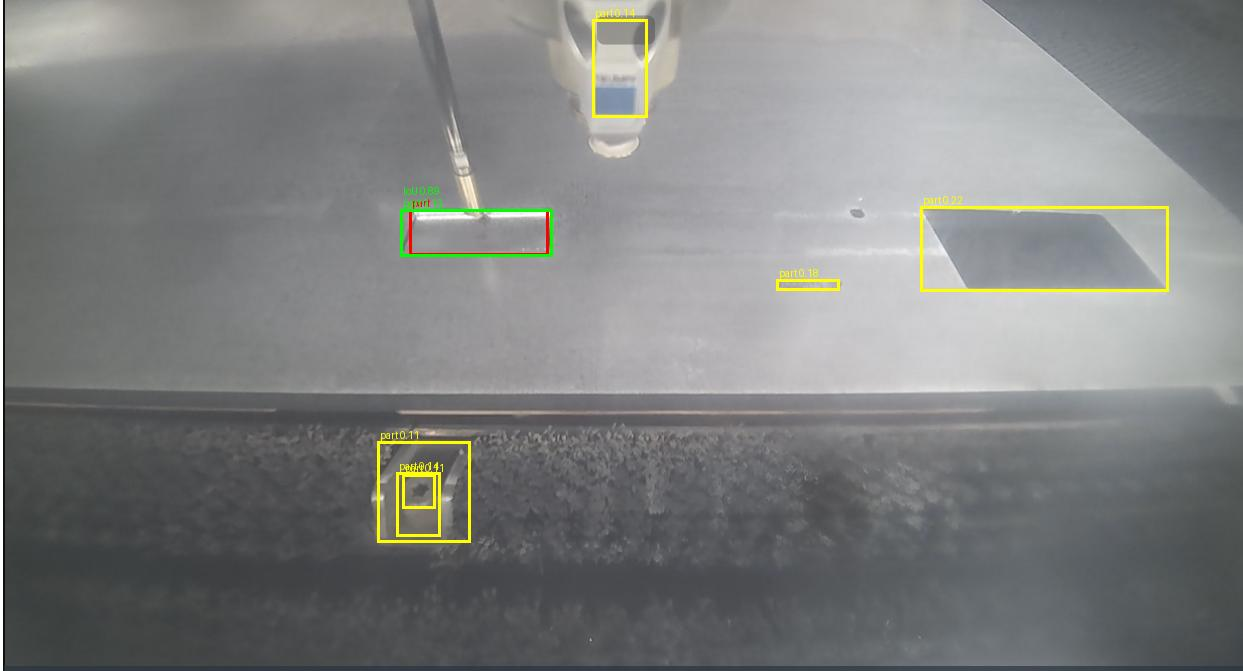
\includegraphics[width=0.9\linewidth]{graphics/example_synthetic_images/Beispiel_Detektion_rtdetr.jpg}
      \caption{Visualisierung einer Vorhersage des \ac{RT-DETR}-Modells mit Datenaugmentierung auf einem realen Bild (\textit{Confidence Threshold 0.1})}
      \label{fig:beispiel_vorhersage_rtdetr}
\end{figure}

\subsection{Zusammenfassung der Evaluationsergebnisse}
Es lässt sich zusammenfassen, dass die \ac{YOLO}-Modelle auf dem synthetischen Datensatz eine gute Leistung erbringen konnten, wobei alle drei Modelle in ihrer Leistung keine signifikanten Unterschiede aufwiesen. Das transformerbasierte Modell hingegen zeigte sowohl auf dem synthetischen als auch auf dem realen Datensatz eine deutlich schlechtere Leistung, trotz dass beide Varianten während des Trainings überraschend schnell konvergierten. Alle trainierten \ac{KI}-Modelle zeigten Schwierigkeiten bei der Übertragung ihrer Leistung auf realen Anwendungsfälle, was den Einfluss des \textit{Domain Gaps} verdeutlicht. Das \ac{YOLO}-Medium-Modell konnte dabei noch die beste Leistung auf dem realen Datensatz erzielen, erbrachte jedoch dennoch keine zufriedenstellende Leistung.

\chapter[Kritische Reflexion und Ausblick]{Kritische Reflexion und Ausblick\footnote{Sprachlich geglättet durch ChatGPT-5}}
\label{chapter:Ergebnisdiskussion}

\section{Auftrag der Arbeit}
Das zentrale Ziel dieser Arbeit war die Entwicklung einer Pipeline zur automatisierten Generierung synthetischer Bilddaten für das Training von \ac{KI}-Modellen zur Fehlererkennung bei Werkzeugmaschinen. Dieses Ziel ergab sich aus der in der Forschungsliteratur beschriebenen Problematik, dass insbesondere im industriellen Kontext häufig nur unzureichende oder einseitige reale Daten für das Training von \ac{KI}-Modellen zur Verfügung stehen.\footnote{Vgl. Kapitel \ref{sec:problemstellung}}

Um diesen Datenmangel zu adressieren, wurde eine Datenpipeline konzipiert, welche eine einfach und flexible Generierung umfangreicher, ausgeglichener und realistischer synthetischer Datensätze ermöglicht. Darüber hinaus sollten verschieden \ac{KI}-Modelle auf diesen generierten Daten trainiert werden, um die Eignung synthetischer Daten zu validieren.

Im praktischen Teil der Arbeit wurde daher eine Simulationsumgebung in \textit{NVIDIA Omniverse} aufgebaut und eine Pipeline zur automatisierten Generierung synthetischer Bilddaten implementiert, bei welcher zentrale Parameter hinsichtlich der Bildqualität, der Anzahl der Bilder und der Simulationsumgebung einfach modifiziert werden konnten. Diese Daten wurden in ein für das Modelltraining geeignete Format überführt und die Eignung und Qualität der generierten Daten durch ein Training von drei Varianten der \ac{YOLO}-Architektur sowie ein transformerbasiertes Modell validiert. Als methodische Grundlage diente dabei das \ac{DSR}-Paradigma, welches es ermöglichte, das entwickelte Artefakt in einem iterativen Prozess zu evaluieren und zu verbessern.


\section{Kritische Reflexion der Methodik und Ergebnisse}

Die Ergebnisse der Evaluation zeigen, dass die entwickelte Pipeline erfolgreich synthetische Bilddaten generieren konnte, welche konsistent waren und sich für das Training von \ac{KI}-Modellen eigneten. Alle trainierten \ac{YOLO}-Modelle konnten auf dem synthetischen Testdatensatz eine gute Leistung erbringen und auch ihr Trainingsverlauf sah vielversprechend aus. Zwar zeigte die transformerbasierten Modelle hier deutlich schlechtere Ergebnisse, dies lässt sich jedoch nicht unmittelbar auf die Qualität der generierten Daten zurückführen, da die CNN-basierten Modelle konsistente Resultate erbrachten. Damit kann die Forschungsfrage der Arbeit, wie synthetische Daten für das Training von \ac{KI}-Modellen zur Fehlererkennung bei Werkzeugmaschinen genutzt werden können und inwieweit die daraus generierten synthetischen Daten für den Einsatz in realen Anwendungsfällen geeignet sind, grundsätzlich beantwortet werden.

Der fehlende Erfolg beim Transfer auf reale Daten kann verschieden Gründe haben und ist nicht zwangsläufig auf die Qualität oder den mangelden Realismus der generierten Daten zurückzuführen. Wie schon in Tabelle \ref{tab:yolo_results} zu sehen ist, erzielte das größte trainierte \ac{YOLO}-Modell auf dem realen Datensatz bessere Ergebnisse als kleinere Modelle. Dies legt nahe, dass die Modellgröße ein entscheidender Faktor für die Übertragbarkeit sein kann. Insbesondere bei transformerbasierten Modellen spielt außerdem die Größe und Vielfalt des Datensatzes eine zentrale Rolle, da ihre Leistung in besonderem Maße von umfangreichen Trainingsdaten abhängt.\footnote{Vgl. \cite[8]{jamil_comprehensive_2022}; \cite[209]{berroukham_vision_2023}} Der Schwerpunkt dieser Arbeit lag außerdem nicht auf der Optimierung der Modelleistung, beispielsweise durch die Ermittlung optimaler Hyperparameter, sondern auf der Konzeption und Umsetzung der Pipeline zur Generierung synthetischer Daten.

Es ergaben sich im Verlauf der Umsetzung und Evaluation des weiteren diverse Herausforderungen und Limitation, welche den Umfang und die Qualität der generierten Daten sowie die Leistung der \ac{KI}-Modelle beeinflusst haben:

\begin{itemize}
    \item \textbf{Rechenleistung und Ressourcen}: Das Training stieß insbesondere bei den größeren Modellen auf Hardware- und Zeitbeschränkungen. Die begrenzte Rechenleistung wirkte sich sowohl auf den Realismus als auch auf den Umfang der generierten Daten aus. Auch die Auswahl der Größe der \ac{KI}-Modelle wurde durch die verfügbare Hardware limitiert, was insbesondere die Übertragbarkeit auf reale Daten beeinträchtigt haben könnte.
    \item \textbf{Umfang und Qualität der Daten}: Der synthetische Datensatz umfasste lediglich eine begrenzte Anzahl von Fehlerfällen, Perspektiven und Variationen. Die Größe des Datensatzes war mit 1.077 Bildern relativ klein, was die Generalisierungsfähigkeit und Leistung der Modelle eingeschränkt haben könnte.
    \item \textbf{Fehlerquellen in der Datengenerierung}: Unerwartete Fehler wie etwa ungewollte Objektrotationen oder fehlerhafte Annotationen durch den \textit{Omniverse Replicator} führten wiederholt zu Verzögerungen.
    \item \textbf{Modellarchitekturen}: Während die \ac{YOLO}-Modelle auf synthetischen Daten konsistente Ergebnisse lieferten, zeigte das transformerbasierte \ac{RT-DETR}-Modell eine deutlich geringere Leistung. Ursachen hierfür können im kleinen Datensatz, in einer unzureichenden oder fehlerhaften Datenaugmentierung sowie in fehlender Expertise bei der Konfiguration von Transformermodellen und deren Hyperparametern liegen.
\end{itemize}

Das \ac{DSR}-Paradigma erwies sich als geeignete Methodik, um die Entwicklung der Pipeline zu strukturieren und iterative Verbesserungen basierend auf den Evaluationsergebnissen vorzunehmen. Es konnten somit Fehler frühzeitig erkannt und korrigiert als auch die Modelleistungen und Datenqualität stetig verbessert werden. Schlussendlich wäre jedoch eine intensivere Auseinandersetzung mit verschiedenen \ac{KI}-Architekturen und deren konkreten Anforderungen an Trainingsdaten, Datenaugmentation und Hyperparameter-Konfigurationen für die Evaluation der Datenpipeline hilfreich gewesen, da aktuell zahlreiche Parameter Einfluss auf die erzielten Ergebnisse haben könnten. Dies war jedoch aufgrund zeitlicher Limitationen nur eingeschränkt möglich. Auch die Anzahl der iterativen Trainings- und Evaluationsdurchläufe wurde durch die zeitlichen Beschränkungen limitiert. Weitere Iterationen hätten die Qualität der Daten sowie die Leistung der Modelle weiter verbessern können.


\section{Implikationen für die Forschung}
Die Ergebnisse machen deutlich, dass der Einsatz synthetischer Daten ein hohes Potenzial bietet, jedoch weitere Forschung notwendig ist, um die Übertragbarkeit auf reale Anwendungsfälle zu verbessern:

\begin{itemize}
    \item \textbf{Effizientere Simulationssoftware}: Die eingesetzte Software \textit{NVIDIA Omniverse} bietet zwar eine hohe Flexibilität und einen hohen möglichen Realismus, ist jedoch sehr ressourcenintensiv.\footnote{Vgl. \cite{noauthor_isaac_nodate}} Alternativ könnte die Nutzung von effizienteren Simulationssoftware wie beispielsweise \textit{Genesis}\footnote{Vgl. \cite{noauthor_genesis-embodied-aigenesis_2025}} untersucht werden, die speziell auf Effizienz und geringere Hardwareanforderungen ausgelegt ist.
    \item \textbf{Größere und realistischere Datensätze}: Für eine bessere Generalisierungsfähigkeit sollten mehr Daten mit höherer Variabilität und höhere Qualität generiert werden. Hierzu zählen zusätzliche Fehlerklassen, variierende Perspektiven sowie realitätsnähere Darstellungen, sodass ein größerer und umfangreicherer Datensatz für das Training der \ac{KI}-Modelle zur Verfügung steht.
    \item \textbf{Leistungsfähigere Modelle}: Die erzielten Ergebnissen deuten darauf hin, dass größere Modelle besser geeignet sein könnten, um den \textit{Domain Gap} zu überbrücken. Dies setzt jedoch eine deutlich höhere Rechenleistung sowie die Möglichkeit für längere Trainingszeiten voraus.
    \item \textbf{Diffusionsmodelle}: Um den Realismus der synthetischen Bilddaten zu erhöhen, ohne die Hardwareanforderugen unverhältnismäßig zu steigern, könnte der Einsatz von Diffusionmodellen eine vielversprechende Möglichkeit darstellen. Hierbei werden synthetisch generierte Bilddaten genutzt und anschließend Oberflächen und Materialien durch den Einsatz eines Diffusionsmodells realistischer gestaltet.\footnote{Vgl. \cite{hadadan_generative_2025}}
    \item \textbf{Hybrides Training}: Eine vielversprechende Möglichkeit besteht darin, synthetische und reale Daten kombiniert einzusetzen. Dabei wird das Modell auf synthetischen Daten trainiert und anschließend ein \textit{Fine-Tuning} auf realen Daten durchgeführt. Ein solches hybrides Training könnte die Generalisierungsfähigkeit der Modelle verbessern und den \textit{Domain Gap} verringern.\footnote{Vgl. \cite[17]{zaripov_creation_2025}}
    \item \textbf{Architekturen}: Die Eignung weiterer Architekturen, wie beispielsweise die eines \ac{HVT}, die Elemente von \ac{CNN}- und Transformer-Ansätzen kombiniert, könnte untersucht werden.\footnote{Vgl. \cite[S. 4 f.]{khan_survey_2023}}
\end{itemize}

Es lässt sich insgesamt feststellen, dass insbesondere in Hinblick auf das Remote Monitoring von Werkzeugmaschinen, der Einsatz von synthetischen Daten eine vielversprechende Möglichkeit und zugleich eine große Chance darstellt. Durch weitere Forschung in diesem Bereich kann die Übertragbarkeit auf reale Anwendungsfälle verbessert werden und die Nutzung synthetischer Daten einen maßgeblichen Beitrag zur automatisierten Fehlererkennung und -klassifizierung leisten, was insbesondere bei der Fernüberwachung von Maschinen von hoher Relevanz ist.

\section{Einordnung und Ausblick}
Trotz der begrenzten Übertragbarkeit auf reale Daten wurde das zentrale Ziel dieser Arbeit erreicht: Die entwickelte Pipeline konnte erfolgreich synthetische Bilddaten inklusive Annotationen generieren und für das Training von \ac{KI}-Modellen aufbereiten. Die gute Performance der \ac{YOLO}-Modelle auf dem synthetischen Datensatz unterstreicht die Konsistenz und Eignung der generierten Daten für das Training solcher Modelle. Die in Kapitel \ref{sec:problemstellung} gestellte Forschungsfrage konnte durch das entwickelte Artefakt, dessen Evaluation sowie kritische Diskussion beantwortet werden.

Die schwache Performance auf realen Daten verdeutlicht jedoch die Auswirkungen des bestehenden \textit{Domain Gaps} und zeigt somit auf konkrete Handlungsfelder für die weitere Forschung auf. Dazu zählen der Einsatz effizienterer Simulationssoftware, eine stärkere Recheninfrastruktur, alternative generative Verfahren (z.B. Diffusionsmodelle) sowie die Untersuchung weiterer Modellarchitekturen und Trainingsansätze, um die Übertragbarkeit von synthetischen Daten auf reale Anwendungsfälle zu verbessern und den \textit{Domain Gap} zu schließen.

Insgesamt bestätigt die Arbeit, dass synthetische Daten ein wertvolles Werkzeug für das Training von \ac{KI}-Modellen darstellen. Ihre erfolgreiche Integration in der industriellen Praxis erfordert jedoch zusätzliche Investitionen in Datenqualität, Modellgröße und Trainingsstrategien.


\startAnhang

\listofanhang
\clearpage

\anhang{Generierung synthetische Daten mithilfe des \textit{Omniverse Replicators} Quellcode}\label{anhang:replicator_code}
\footnote{Erstellung mit Unterstützung von ChatGPT-5 und Claude Sonnet 4}
\lstset{
  language=Python,
  basicstyle=\ttfamily\small,
  numbers=left,
  numberstyle=\tiny,
  stepnumber=1,
  numbersep=5pt,
  breaklines=true,        % Zeilenumbruch aktivieren
  breakatwhitespace=false, % nur an Leerzeichen umbrechen
  tabsize=4,
  showstringspaces=false,
  commentstyle=\color{gray}
}
\lstinputlisting{includes/code/replicator_script.py}

\anhang{Erstellung des Datensatzes für die Modelltrainings Quellcode}\label{anhang:datensatz_erstellen_code}
\lstset{
  language=Python,
  basicstyle=\ttfamily\small,
  numbers=left,
  numberstyle=\tiny,
  stepnumber=1,
  numbersep=5pt,
  breaklines=true,        % Zeilenumbruch aktivieren
  breakatwhitespace=false, % nur an Leerzeichen umbrechen
  tabsize=4,
  showstringspaces=false,
  commentstyle=\color{gray}
}
\lstinputlisting{includes/code/create_ds.py}

\anhang{Training der \ac{YOLO} Modelle Quellcode}\label{anhang:yolo_code}
\lstset{
  language=Python,
  basicstyle=\ttfamily\small,
  numbers=left,
  numberstyle=\tiny,
  stepnumber=1,
  numbersep=5pt,
  breaklines=true,        % Zeilenumbruch aktivieren
  breakatwhitespace=false, % nur an Leerzeichen umbrechen
  tabsize=4,
  showstringspaces=false,
  commentstyle=\color{gray}
}
\lstinputlisting{includes/code/train_yolo.py}

\anhang{Training of \ac{RT-DETR} Model Source Code}\label{anhang:rt_detr_code}
\lstset{
  language=Python,
  basicstyle=\ttfamily\small,
  numbers=left,
  numberstyle=\tiny,
  stepnumber=1,
  numbersep=5pt,
  breaklines=true,        % Zeilenumbruch aktivieren
  breakatwhitespace=false, % nur an Leerzeichen umbrechen
  tabsize=4,
  showstringspaces=false,
  commentstyle=\color{gray}
}
\lstinputlisting{includes/code/train_rtdetr.py}

\anhang{Evaluation der trainierten \ac{YOLO}-Modelle und des \ac{RT-DETR}-Modells Quellcode}\label{anhang:evaluation_models_code}
\lstset{
  language=Python,
  basicstyle=\ttfamily\small,
  numbers=left,
  numberstyle=\tiny,
  stepnumber=1,
  numbersep=5pt,
  breaklines=true,        % Zeilenumbruch aktivieren
  breakatwhitespace=false, % nur an Leerzeichen umbrechen
  tabsize=4,
  showstringspaces=false,
  commentstyle=\color{gray}
}
\anhangteil{Evaluation der \ac{YOLO}-Modelle auf synthetischen und realen Bilddaten Quellcode}
\label{anhang:evaluation_yolo_code}
\footnote{Erstellung mit Unterstützung von ChatGPT-5 und Claude Sonnet 4}
\lstinputlisting{includes/code/evaluate_yolo.py}

\anhangteil{Evaluation des \ac{RT-DETR}-Modells auf synthetischen und realen Bilddaten Quellcode}
\label{anhang:evaluation_rtdetr_code}
\footnote{Erstellung mit Unterstützung von ChatGPT-5 und Claude Sonnet 4}
\lstinputlisting{includes/code/evaluate_rtdetr.py}


\anhang{Metriken zur Evaluation der \ac{YOLO}-Modelle}\label{anhang:training_verlauf}
\anhangteil{Trainingsverlauf des Nano Modells}\label{anhang:training_nano}
\begin{figure}[htb]
\centering
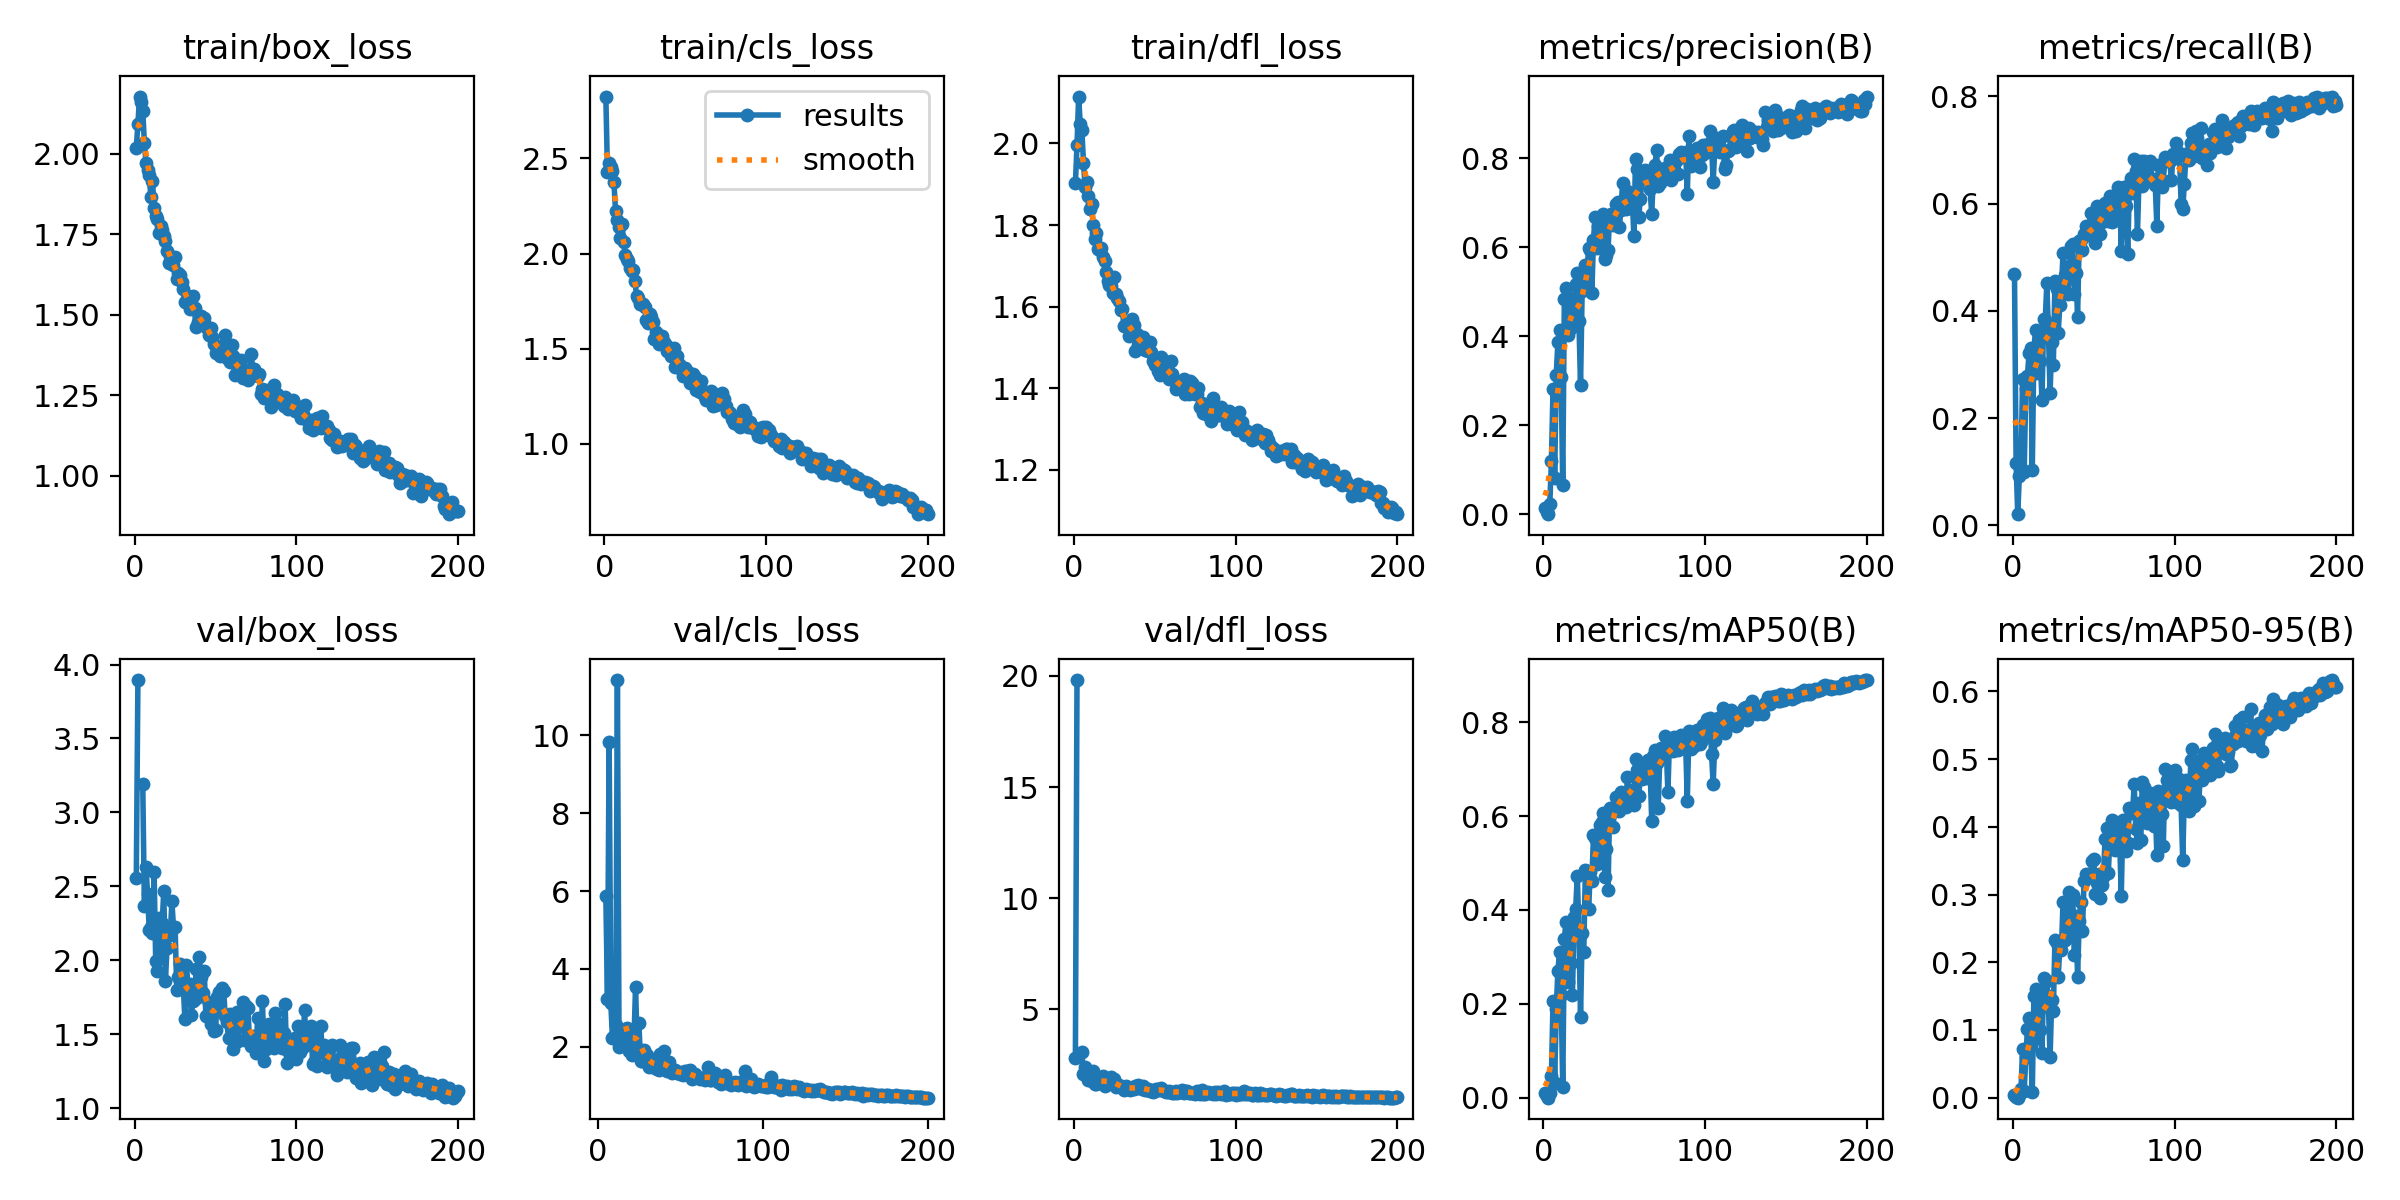
\includegraphics[width=0.9\linewidth]{graphics/yolo_eval/model_n/results.png}
\caption{Verlauf von Metriken während des Trainings des \ac{YOLO} Modells Nano}
\end{figure}

\anhangteil{Trainingsverlauf des Small Modells}\label{anhang:training_small}
\begin{figure}[htb]
\centering
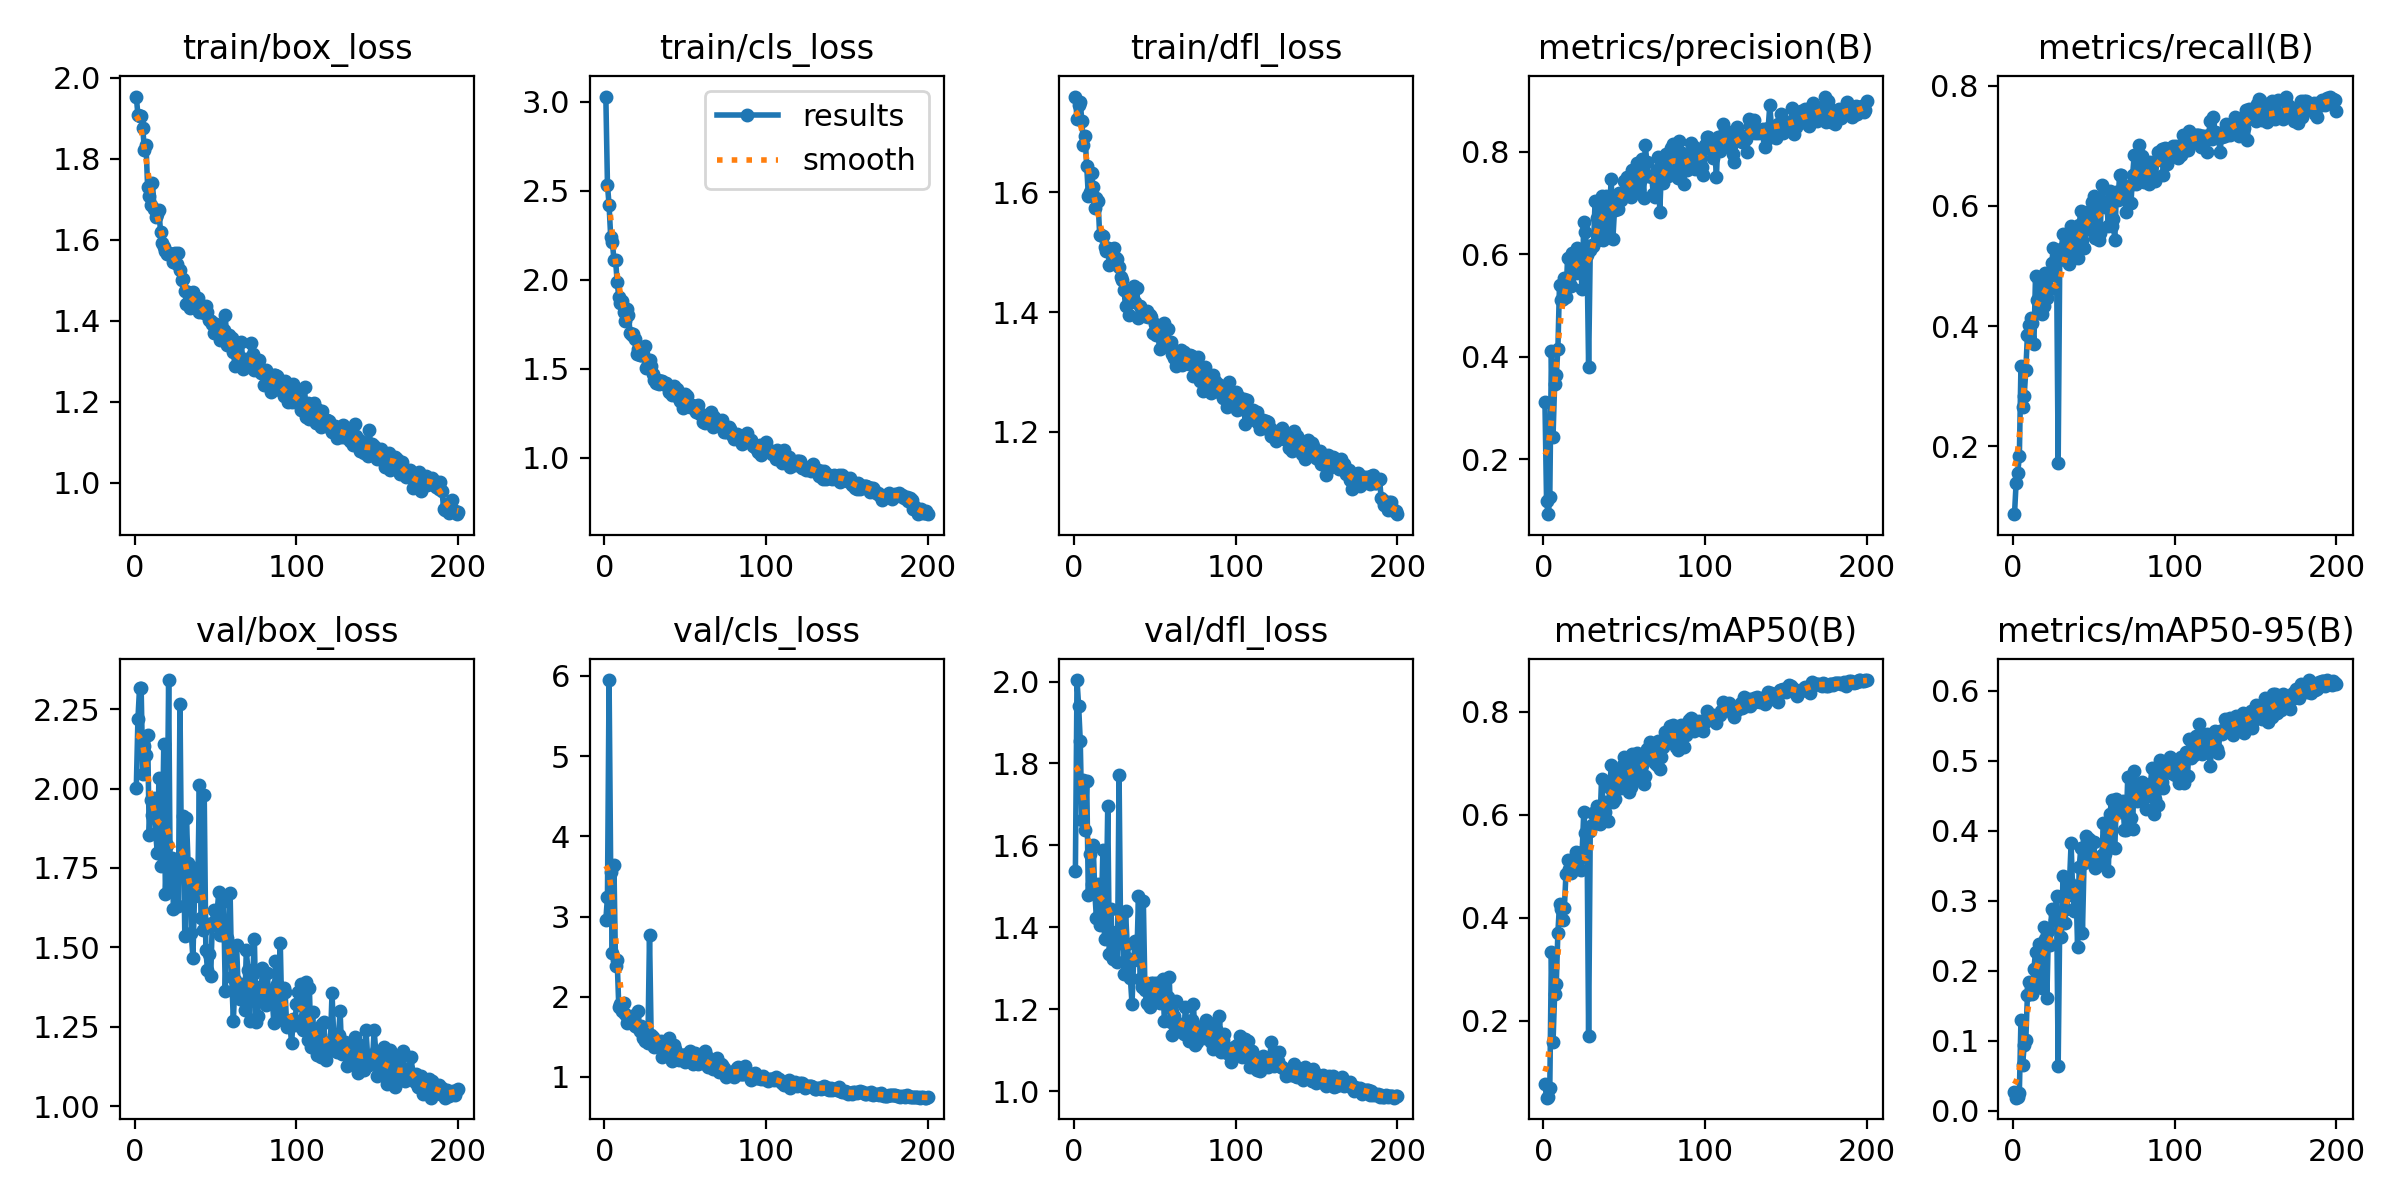
\includegraphics[width=0.9\linewidth]{graphics/yolo_eval/model_s/results.png}
\caption{Verlauf von Metriken während des Trainings des \ac{YOLO} Modells Small}
\end{figure}

\anhangteil{Precision-Recall-Kurve für das Small Modell}\label{anhang:pr_curve_small}
\begin{figure}[htb]
\centering
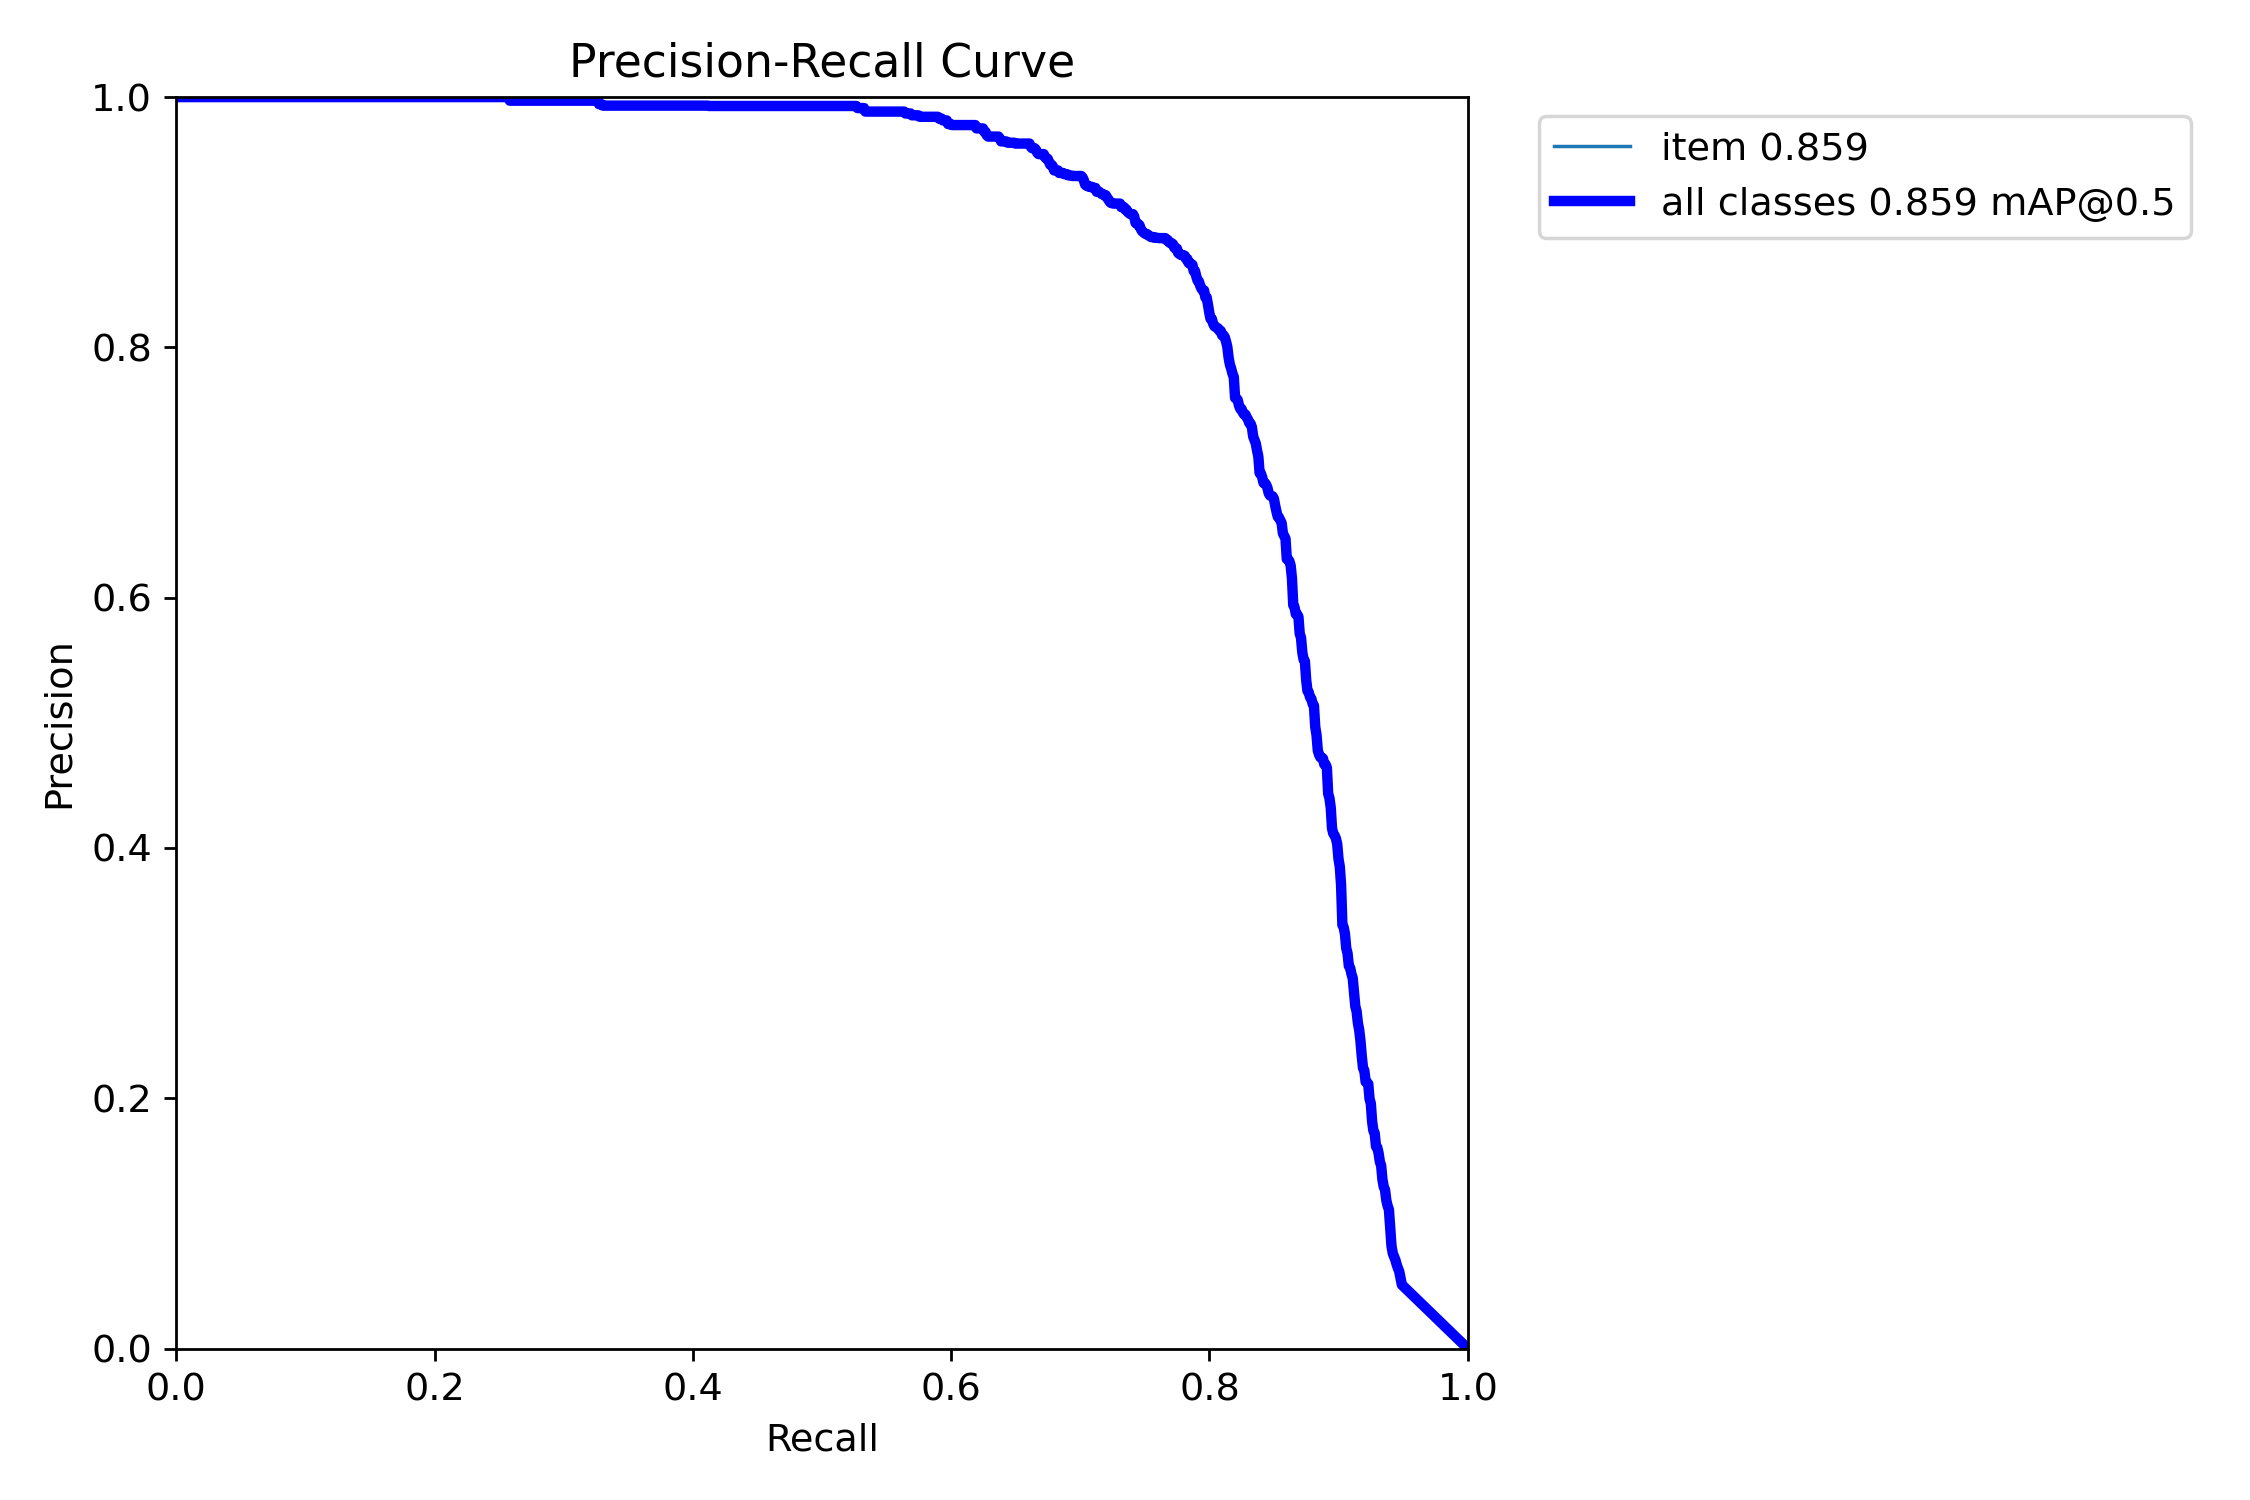
\includegraphics[width=0.9\linewidth]{graphics/yolo_eval/model_s/BoxPR_curve.png}
\caption{Precision-Recall-Kurve des \ac{YOLO} Small Modells}
\end{figure}
%%% Ende des eigentlichen Inhalts %%%


%%% Quellenverzeichnisse (keine Anpassung nötig) %%%
\clearpage
\literaturverzeichnis
%%% Ende Quellenverzeichnisse %%%


%%% Erklärung (keine Anpassungen nötig) %%%
% steht ganz am Ende des Dokuments
\cleardoublepage
\clearpage
\thispagestyle{plain} % oder empty, je nach Vorgaben

{\large\textbf{Erklärung zur Verwendung von \acs{KI}-Systemen}}\par\vspace{0.8\baselineskip}

Ich erkläre, dass ich
\begin{itemize}[leftmargin=2.2em,label=\checkedbox,itemsep=0.45\baselineskip]
  \item mich aktiv über die Leistungsfähigkeit und Beschränkungen der in meiner Arbeit eingesetzten \ac{KI}-Systeme informiert habe;
  \item alle Inhalte aus wissenschaftlich anerkannten Quellen entnommen und entsprechend gekennzeichnet habe; alle Inhalte unter Anwendung wissenschaftlicher Methoden im Rahmen der vorliegenden Arbeit von mir selbst entwickelt wurden;
  \item mir bewusst bin, dass ich als Autorin dieser Arbeit die Verantwortung für die in ihr gemachten Angaben und Aussagen trage.
\end{itemize}

\vspace{0.6\baselineskip}
Bei der Erstellung der Arbeit habe ich die folgenden auf \ac{KI} basierenden Systeme in der im Folgenden dargestellten Weise benutzt:\par\vspace{0.6\baselineskip}

\noindent
\begin{tabularx}{\textwidth}{|p{0.28\textwidth}|p{0.26\textwidth}|Y|}
\hline
\textbf{Arbeitsschritt} & \textbf{Eingesetzte \ac{KI}-Systeme} & \textbf{Beschreibung der Verwendungsweise} \\
\hline
Literatursuche & Consensus & Teilweise unterstützender Charakter für die Auffindung relevanter Literatur \\
\hline
Codeerstellung und -unterstützung & ChatGPT-5, Claude Sonnet 4 & Unterstützung bei Code-Vervollständigungen und Fehlersuche \\
\hline
Formulierung des Textes der Arbeit & ChatGPT-5 & Sprachliche Unterstützung in Form von Formulierungsvorschläge zur sprachlichen Präzisierung und Variation \\
\hline
Redigieren des Textes & ChatGPT-5 & Unterstützung bei der sprachlichen Glättung und Verbesserung der Lesbarkeit \\
\hline
\end{tabularx}

\vspace{1.6cm}

\noindent\rule{7cm}{0.4pt}\\
\small Ort, Datum, Unterschrift
\clearpage
\clearpage

\thispagestyle{empty}

{\LARGE\textsf{\textbf{\DEoEN{Erklärung}{Declaration}}}\bigskip}

% \typMeinerArbeit und \themaMeinerArbeit werden in config.tex definiert
\DEoEN{%
Ich versichere hiermit, dass ich die vorliegende Arbeit mit dem Thema: \emph{\themaMeinerArbeit} selbstständig verfasst und keine anderen als die angegebenen Quellen und Hilfsmittel benutzt habe.
Ich versichere zudem, dass die eingereichte elektronische Fassung mit der gedruckten Fassung übereinstimmt.%
}{%
I hereby insure that I have personally authored this thesis with the topic: \emph{\themaMeinerArbeit} and have used no sources and aids other than those indicated. I also insure that the submitted electronic version corresponds to the printed version.%
}

\vspace{3cm}

\begin{center}
\begin{tabular}{ccc}
(\DEoEN{Ort, Datum}{place, date}) & \hspace{0.3\linewidth} & (\DEoEN{Unterschrift}{signature})
\end{tabular}
\end{center}


\end{document}
